\documentclass[a4paper,12pt]{report}

\usepackage{times}
%\usepackage[dvipdfmx]{graphicx}
\usepackage{amsmath}
\usepackage{amssymb}
\usepackage{amsfonts}
\usepackage[ruled,linesnumbered]{algorithm2e}
\usepackage{cite}
\usepackage{url}
\usepackage{listliketab}
\usepackage{lipsum}
\usepackage{calc}
\usepackage{multirow}
\usepackage{here}
\usepackage{amsthm} 
\usepackage{graphicx}
\usepackage{epstopdf}
\usepackage{lscape}
\usepackage{tikz}
\usepackage{esvect}
\usepackage{wrapfig}
\usepackage{tabularx}
\usepackage{rotating}
\mathchardef\mhyphen="2D
\usepackage{afterpage}
\usepackage{tabularray}
\usepackage{makecell}
\usepackage{booktabs}
\usepackage{multirow}
\usepackage{multicol}
\usepackage{csquotes}

\newcommand{\tc}{T$_{c}$}

\ifpdf
  \DeclareGraphicsExtensions{.eps,.pdf,.png,.jpg}
\else
  \DeclareGraphicsExtensions{.eps}
\fi


\usepackage{enumitem}
\setlist[enumerate]{leftmargin=.5in}
\setlist[itemize]{leftmargin=.5in}


\usepackage[subrefformat=parens,labelformat=parens]{subfig}
%\usepackage{algorithm}
%\usepackage{algorithmic}
\usepackage{iitem}
%\renewcommand{\algorithmicrequire}{\textbf{Input:}}
%\renewcommand{\algorithmicensure}{\textbf{Output:}}
\usepackage{url}
\newtheorem{Definition}{\bf Definition}[section]
\newtheorem{Theorem}{\bf Theorem}[section]
\newtheorem{Lemma}{\bf Lemma}[section]
\newtheorem{Proof}{\bf Proof}[section]
\newcommand{\fig}[1]{{\gt fig.\ref{#1}}}
\newcommand{\eq}[1]{{\gt eq.\ref{#1}}}
\newcommand{\minmin}{\mathop{\rm min}\limits}
\newcommand{\bhline}[1]{\noalign{\hrule height #1}}  
\newcommand{\bvline}[1]{\vrule width #1}  

\usepackage{amsopn}
\DeclareMathOperator{\diag}{diag}

% \usepackage[top=20truemm,bottom=25truemm,left=25truemm,right=25truemm]{geometry}


\newtheorem{definition}{\textbf{Definition}}
\newtheorem{lemma}{\textbf{Lemma}}
\newtheorem{observation}{\textbf{Observation}}
\newtheorem{example}{\textbf{Example}}
\newtheorem{theorem}{\textbf{Theorem}}
\newtheorem{problem}{\textbf{Problem}}
% \newtheorem{proof}{\textbf{Proof}}
\newcommand{\argmax}{\mathop{\rm arg~max}\limits}
\newcommand{\argmin}{\mathop{\rm arg~min}\limits}

\setcounter{tocdepth}{3} %目次の深さ, toc: table of contents
\setcounter{page}{-1}

\setlength{\oddsidemargin}{9mm}
\setlength{\evensidemargin}{9mm}
\setlength{\topmargin}{5mm}
\setlength{\textwidth}{140mm}
\setlength{\textheight}{200mm}

\setlength{\parskip}{1em}
\setlength{\topsep}{0em}

\renewcommand{\baselinestretch}{1.0}

\newcommand{\vect}[1]{\mbox{\boldmath ${#1}$}}
\newcommand{\mat}[1]{\mbox{\bf {#1}}}
\newcommand{\unitvect}{\mbox{\bf 1}}

\newcommand{\eat}[1]{}

\newcommand{\authorlarge}{
  \vspace{35mm}\\
  {\LARGE March 2024}\\
  \vspace{10mm}\\
  {\Huge Luca Foppiano}
}
\newcommand\normx[1]{\left\Vert#1\right\Vert}
\makeatletter
\newcommand{\maketitleouter}{\newpage
\null
\vskip 5em 
\begin{center}
{\LARGE \@title \par} \vskip 1.5em {\large \lineskip .5em
\begin{tabular}[t]{c}\authorlarge
\end{tabular}\par}
\vskip 1em {\large \@date} 
\end{center}
\par
\vskip 1.5em
\thispagestyle{empty}
}
\makeatother

\title{\vspace{-15mm}{Automated Extraction and Curation of Materials Information from Scientific Literature}\vspace{65mm}}
\author{
  {\Large Graduate School of Science and Technology}\vspace{4mm}\\
  {\Large Degree Programs in Systems and Information Engineering}\vspace{4mm}\\
  {\LARGE University of Tsukuba}\vspace{10mm}\\
  {\LARGE March 2024}\\
  \vspace{10mm}\\
  {\Huge Luca Foppiano}
}
\date{}

\renewcommand{\baselinestretch}{1.}

\usepackage[colorlinks = true, linkcolor = black, citecolor=black]{hyperref}%

\begin{document}

\maketitleouter
\maketitle

% \thispagestyle{empty} % no page number
% \include{01_cover}

\pagenumbering{roman} % page number : i, ii, iii, iv
\setcounter{page}{1}
%\newpage\thispagestyle{empty}\mbox{}\newpage



\addcontentsline{toc}{chapter}{Abstract}
\begin{abstract}

The scientific literature, containing vast human knowledge, is rapidly expanding, posing challenges in organising and retrieving information. 
Big data methods aid in uncovering patterns and making predictions and have been long applied in Chemistry and Biology, with other disciplines, such as Materials Science falling behind.
Materials Informatics (MI) is a discipline that leverages computational power to accelerate research in Materials Science by employing techniques like Density Functional Theory (DFT) computations and Machine Learning (ML) for material discovery. 
Despite advances, limited experimental datasets, like SuperCon, hinder progress. 
SuperCon, a complex database for superconductor materials, faces challenges in consistent data collection. 
Automated processes are needed for timely data extraction from new publications, and manual curation, prone to errors, requires careful tools and feature selection.

In this dissertation, we propose an end-to-end pipeline for extracting material information from scientific literature to improve the efficiency and quality of materials databases.
Our work aims to increase the automated tasks to reduce the dependency on human intelligence to the minimum. 
The main contributions consist of developing ML-based models for recognising complex materials expressions and other information from scientific text that is obtained directly from PDF documents. 
Material expressions are further processed with a parser that decomposes granular information such as name, formulas, doping, shape etc. 
The extraction of properties is performed by combining with a general model for extracting physical quantities and measurements, called Grobid-quantities which support the identification and normalisation of units to the SI system. 
For evaluation and training, we developed SuperMat, a dataset of 142 superconductor articles. The dataset contains both entities and relations between them, and it was validated by domain experts.  
The automatic process collected a database with over 40,000 extracted material-properties records from the related scientific articles from ArXiv. 
Finally, we proposed a curation interface to validate extracted data by combining an enhanced PDF viewer and a simple and sleek interface. Overall, the use of such an interface as compared with the traditional manual approach improved precision by 6\% and recall by 47\%. 

The models, dataset, and interface developed in this work will help increase the automation and accuracy of populating materials databases like SuperCon from the scientific literature.

\end{abstract}
\newpage\thispagestyle{empty}\mbox{}\newpage


\pagebreak
\tableofcontents


\pagebreak
\addcontentsline{toc}{chapter}{List of Figures}
\listoffigures

\pagebreak
\addcontentsline{toc}{chapter}{List of Tables}
\listoftables

\pagebreak
\setcounter{page}{1}
\pagenumbering{arabic} % page number : 1,2,3

\chapter{Introduction}
% Dependency between concepts
% -> materials science 
% -> Materials informatics 
% -> superconductivity 
% -> SuperCon
% -> Computational science 

% General introduction: 
% -> TDM 
% -> ML

% Materials science 
Materials science is a multidisciplinary field at the intersection of physics, chemistry, and engineering, dedicated to understanding, designing, and manipulating materials for a myriad of real applications. 
Central to this discipline is the exploration of the structure, properties, and performance of materials, ranging from metals and ceramics to polymers and composites. By delving into the microscopic and atomic scales, materials scientists seek to uncover the fundamental principles that govern a material's behaviour and tailor its properties to meet specific technological needs. 
This field plays a critical role in advancing technology and innovation, as discoveries in materials science often lead to the development of new materials with enhanced functionalities, improved performance, and novel applications across industries.

% Materials informatics 
Historically, breakthroughs in materials science often resulted from chance discoveries and unexpected observations, a process driven by serendipity and relying on trial and error. 
However, with the advent of advanced computational tools, machine learning, and big data analytics, materials informatics (MI) has emerged as a transformative methodology. 
Materials informatics is a multidisciplinary field that leverages computational methods, data science, and informatics techniques to accelerate the discovery and design of new materials, identify patterns, and predict material properties with unprecedented accuracy. 
Materials informatics not only expedites the discovery of novel materials but also enhances our understanding of complex relationships between structure, composition, and performance. 
This approach allows for a more efficient and systematic exploration of the vast material space, potentially leading to breakthroughs in fields such as electronics, energy, healthcare, and beyond. 

% Look at other fields 
In comparison of MI with well-established fields like computational chemistry and biology, we can discern not only the unique contributions of each discipline but also the collective progression towards harnessing computational power for transformative advancements in science and technology.
Computational chemistry is the earliest among the three, with its roots tracing back to the mid-20th century. The development of computational chemistry gained momentum with the advent of digital computers, and it has evolved significantly over the decades. Computational chemistry involves the application of theoretical methods and simulations to study the structure, properties, and behaviour of molecules, making it a well-established and mature field.
Computational biology, on the other hand, gained prominence later, particularly with the explosion of biological data in the post-genomic era. The field began to flourish in the late twentieth century and has since grown rapidly. Computational biology encompasses a broad range of techniques, including bioinformatics, molecular dynamics simulations, and systems biology, to model and analyse biological processes at various levels of complexity.
Materials informatics is a more recent entrant compared to computational chemistry and biology. Although the idea of using informatics approaches for material discovery has been around for some time, the field has gained significant traction over the past few decades, especially with the rise of advanced computing capabilities and the availability of large materials databases. 

Materials Informatics (MI) is founded on two key techniques: Density Functional Theory (DFT) computations and a data-driven approach using Machine Learning (ML). DFT computations, a core aspect of quantum mechanics simulations, delve into a material's electronic structure and properties at the atomic and molecular levels, providing a precise understanding that complements experimental data. On the other front, the data-driven approach utilises ML algorithms, from regression models to neural networks, for the analysis of extensive materials datasets. 
These algorithms decode patterns and correlations, enabling researchers to predict the properties of new materials or optimise existing ones. 
This combined approach, which integrates quantum-level insights with data-driven predictive modelling, accelerates the materials discovery process, facilitating the efficient exploration of diverse materials spaces.

Data-driven methods have significantly contributed to the design of new materials across various sub-domains, such as magneto-caloric, thermoelectrics, and superconductor materials. Despite the impactful role of these methods, a notable challenge lies in the limited availability of experimental datasets. 
Currently, the primary sources for such datasets in inorganic materials are Pauling File~\cite{Blokhin2018ThePF_paulingFile}, Starrydata~\cite{katsura2019data}, and SuperCon~\cite{ishii2023structuring}. 
The use of these databases highlights the need to broaden and diversify experimental data, improving the effectiveness and applicability of data-driven approaches in materials design. The addition of these datasets is crucial to advance the field, promote innovation, and expand the scope of materials discovery through data-driven methodologies.
SuperCon is the standard database for superconductor materials and it has been developed and manually maintained by NIMS since 1987. 
It consists of records of materials reported in scientific experiments and a large set of measured properties. 

A superconductor is a material that, when cooled below a critical temperature, exhibits zero electrical resistance and the expulsion of magnetic fields. This phenomenon, known as superconductivity, occurs in a variety of materials, with many of them requiring extremely low temperatures, often close to absolute zero, to manifest this unique behaviour. The critical temperature at which superconductivity emerges varies depending on the material. Superconductors have numerous applications, notably in the field of electrical engineering. They are utilised to create powerful electromagnets for applications such as magnetic resonance imaging (MRI) machines, particle accelerators, and magnetic levitation systems. Superconductors also play a crucial role in the development of high-speed, energy-efficient power transmission lines, since they can carry large currents without any loss. The potential for quantum computing and more efficient electronic devices is another area where superconductors are actively being explored, showcasing the interdisciplinary nature of their applications in physics, materials science, and technology.

SuperCon hosts about 32,000 materials records and a complex schema with about 200 properties, some of which have not been consistently collected~\cite{sommer20223dsc}. 
For example, the pressure applied to obtain superconductivity was reported in only 16 records; however, its studies and experiments date back to the 1970s, but it became more popular only at the beginning of the 21st century.  
However, SuperCon has been widely recognised for its quality and has been the data source for many attempts to design models that can predict Tc~\cite{stanev_machine_2017, le2020critical, Hamlin2019SuperconductivityNR}. 

However, using ML to predict Tc has some criticality that needs to be considered. 
The models have an intrinsic applicability domain, which means that predictions are limited to the patterns and trends encountered in the training set. 
This can lead to significant selection bias, making the models ineffective when applied to materials constituted by different compounds (or belonging to different classes). 
The variety of training data to be used should contain a relevant amount of non-superconductors materials to avoid training a model biased toward the assumption that a Tc always exists and render it ineffective when applied to new materials.
Now, the definition of non-superconductivity is tricky: if no superconducting critical temperature has been found, does not mean that one does not exist. It might be outside the range of current technological instruments. 
This leads to a conundrum when delving into the data: ignoring compounds with no reported Tc and maybe disregarding a potentially important part of the dataset for the sake of simplicity.
Simplifying too much could lead to an incomplete understanding of the factors that determine superconductivity and limit the ability to predict Tc accurately. 
Generally, in addition to these considerations, several SuperCon-related works attempted to integrate complementary data from other datasets. 
However, at the time of writing, only~\cite{sommer20223dsc} has aimed to directly enhance SuperCon.  
They successfully enhanced 9150 records with crystal structures from experimental results stored in the Inorganic Crystal Structure Database (ICSD). 
This recent work indicates that the SuperCon dataset continues to play a pivotal role in the landscape of superconductor research.

\section{Motivation}

The number of publications in superconductor research remained stable in the last 10 years\footnote{analysed on arXiv statistics on cond-mat category \url{https://info.arxiv.org/about/reports/submission_category_by_year.html}}.
It is reasonable to expect that future breakthroughs in superconductor research will be achieved through materials informatics, given its growing importance, and an updated SuperCon is to be considered a necessary condition. 

Two main challenges that SuperCon is facing motivate our work. 
The manual approach employed for compiling SuperCon is proving to be increasingly demanding in keeping up with the influx of new publications on time. The reliance on manual labour for dataset curation becomes a growing obstacle, as it demands specialised skills that are not readily available in the market. As the field of superconductor research evolves, the need for more efficient and scalable methods becomes apparent.
An automatic process is necessary to streamline and improve the population of SuperCon. 
The outline of the process comprises the ingestion of entire documents or text and the identification of materials and relative proprieties.  
In a small-scale preliminary assessment, we analysed the problem, identified several challenges to overcome, and proposed a data extraction framework~\cite{foppiano2019proposal}.

The expressions that identify materials are complex and lengthy and their identification in the scientific literature poses several challenges.
Furthermore, the strict definition of what a material cannot be expressed in a synthetic sentence is valid for the whole discipline: There are differences between subdomains in materials science that make this process highly dependent on domain experts.

A material may be expressed in a multitude of partially overlapping definitions: as a single material, a single sample, a family, or a class.
Alternative approaches to naming exist, including the use of commercial names or sample designations, often arbitrarily chosen by researchers. Chemical formulas can be presented as stoichiometric expressions within these three categories, with possibilities such as Y-111 or (A, B) C1 D2. Examples of standard names include Oxygen or Magnesium Diboride, while some adopt abbreviated forms like Yttrium Barium Copper Oxide (YBCO). These varied strategies provide a range of options for nomenclature within the domains of chemistry and materials science, while the conventional method primarily involves the use of chemical formulas.

A class of materials refers to a broader category that shares certain fundamental characteristics or properties. Materials in the same class might be characterised by common structural features, electronic configurations, or other common traits that make them suitable for investigation. 
A family usually implies a more specific grouping that shares a closer genetic or compositional relationship. A set of materials with similar chemical compositions, crystal structures, or electronic configurations. 
A sample is just an arbitrary name chosen by the researchers which can overlap any of the previous definitions. 
To make things more complicated, all these definitions are not strictly enforced and may fluctuate from one laboratory to another. 
In many papers, the authors talk about "high-Tc cuprates" referring to materials in the class of cuprates that also have high-Tc. Such a definition is fallacious and not robust, as it does not clearly describe which materials are included: \textit{"How high should be Tc to be considered 'high'?"}.

Manual curation remains a necessary component, but it does not guarantee complete elimination of errors. As reported by~\cite{sommer20223dsc}, their investigation identified over 10,000 duplicated records within the SuperCon dataset at the time of their study, revealing instances where certain properties were inadequately populated. 
This underscores the inherent challenges and limitations associated with relying solely on manual efforts for data curation, emphasising the imperative to adopt more robust and automated strategies to enhance the accuracy and comprehensiveness of the SuperCon dataset.
The necessity of a curation-centric user interface and tools that allow for the reduction of the manual bottleneck to a few minor actions, leaving to the automation of the tedious task of identifying main data in scientific publications.


\section{Problem definition}

Looking at the current situation, NIMS is facing multiple challenges in maintaining SuperCon: a) updating the database is becoming more expensive and b) it is difficult to steer it to accommodate the extraction of different properties. 
First, collaboration with domain experts becomes imperative because they provide both validation and guidance. 
This collaborative effort is challenging due to different work methodologies; however, it facilitates the gathering of methodologies that can be shared between disciplines, fostering a comprehensive and cohesive solution.
The construction of an automatic process is needed to accelerate the extraction of information from scientific papers. In this dissertation, we discuss our work including the main contributions. 

\section{Contributions}

\subsection{Extraction from full-text body of PDF documents}
% PDF document extraction
One pivotal facet of the problem involves the exploration of extracting information from PDF documents, a novel approach not previously employed in related works that predominantly relied on web scraping or publisher API access. 
The latter methods are often hindered by the necessity of agreements with publishers, making the gathered content difficult to share and challenging to replicate.
Using the abundance of open-access data, the ability to extract insights from PDF documents opens avenues for application in diverse use cases. 
The main motivation is rooted in the frequent presence of experimental results in related works, thereby enhancing the potential for recall compared to extraction solely from abstracts. 
However, it is acknowledged that abstracts, being synthetic and possessing a simpler structure, also play a role in data extraction.


\subsection{Extraction of Materials and properties}



\subsection{Extraction of measurement and physical quantities}
% Grobid quantities
As the project is developed around SuperCon we face the challenge to think in a general way, for example considering possible evolution in the properties that are needed, or application in different domains. For this reason, the extraction of properties and conditions needs to be decoupled from any specific domain and addressed in a specific project focused on measurements and physical quantity identification.
This is facilitated by its generic applicability across scientific disciplines. 

\subsection{Parsing long complex materials sequences}

\subsection{SuperMat: a linked annotated dataset of superconductors research papers}
% SuperMat
A critical gap identified in existing resources is the absence of datasets consolidating relevant entities such as materials, conditions, properties, and their interrelations. 
Currently, no dataset offers a centralised solution for machine learning models, considering the intricate and inconsistent terminology prevalent in this domain. 
To rectify this deficiency, constructing a dataset is deemed imperative, forming the foundation for a methodology that involves iterative data collection and correction. This dissertation contributes to this endeavour by expanding the data set for superconductor materials. 
The inclusion of measurement methods, which enable the selection of experimental properties, and the incorporation of applied pressure, an underexplored area, holds the potential to pave the way for groundbreaking advancements soon.


\subsection{Curation workflow and interface}



\chapter{Related work}
\label{cha:related_work}
\chapter{Related work}
This chapter is divided into different contributions and aspects of this research, organised from basic to specific and temporary. 
This section begins to illustrate the related work to properties and measurement extraction. We then discuss the relative work in materials science. 

\section{Machine Learning}

\cite{stanev_machine_2017} used data from SuperCon in combination with ICSD and AFLOW. 
Only a small subset of materials in SuperCon overlap with those in the ICSD: about 800 with finite Tc and <600 are contained within AFLOW. 
The AFLOW Online Repositories contain calculated properties, but the DFT results have been extensively validated with observed properties. 
The work uses this subset of materials to incorporate structural/chemical information and electronic properties from the AFLOW Online Repositories into their models. 
They predicted about 2000 compounds as candidate superconductors, with the vast majority being cuprates or compounds containing copper and oxygen. 
There were also some materials related to iron-based superconductors, as well as 35 members that were not obviously connected to any high-temperature superconducting families.


\section{Deep Learning}

\subsection{Recurrent Neural Networks}
\cite{lample2016neural} propose a new neural architecture for NER with an architecture based on a bi-directional set of LSTM chains. 
Bi-directional indicates that the text is computed from left to right (forward LSTM) and from right to left (backward LSTM). 
Such architecture can incorporate information that is usually captured by hand-crafted features, and/or gazetteers. 
Such architecture takes in input two types of word representation: character-based word representation, calculated from the supervised corpus and unsupervised word representation, which is learned from unsupervised corpora. 
Unsupervised word representations discussed were word2vec~\cite{mikolov2013efficient} but they can be used also more recent ones: fasText~\cite{joulin2016fasttext}, GloVe~\cite{pennington2014glove}.

\cite{peters2018deep} Propose a new type of deep contextualised word representation that models a) complex characteristics of word use, and b) uses words across linguistic contexts (polysemy). 
The solution proposed provides word representation calculated from the entire sequence. The network is composed of two bidirectional LSTM layers of dimensions 4096 x 512. 
The two layers work complementary: one that computes left-to-right the probability of the next token based on the previous, and another right-to-left.
This work also observes several important aspects. A) Instead of outputting the layer from the last layer, averaging with a coefficient all weights from all layers improves results in downstream tasks. B) In such a network, lower levels capture information about aspects of syntax while higher levels capture context-dependent aspects (semantic). C) Including the ELMo embeddings in the output as well as in the input improves tasks that use the attention layer after the RNN, while it does not help for other types of tasks.  


\subsection{Transformers}

(Devlin et al, 2019) \cite{devlin2018bert} introduce BERT (Bidirectional Encoder Representation Transformer). 
While pre-trained language models have been discussed already in previous work~\cite{radford2018improving}, and can be exploited in two main ways: features-based or fine-tuning. 
BERT aims to improve the fine-tuning approach and to solve the limitation of existing left-to-right language models, where each token can attend only to previous tokens in the self-attention layers~\cite{vaswani2017attention} of the Transformers architecture. 
BERT introduces an MLM (Masked Language Model) pre-training objective, where it randomly masks tokens in training examples and tries to predict them using the full context. This enables to use of both left and right context and pre-trains a fully Bidirectional Transformer.
Using the original transformer architecture~\cite{vaswani2017attention}, they define BERT\textsubscript{BASE} with L=12, H=768 and A=12 (110M parameters) and BERT\textsubscript{LARGE} as L=24, H=1024 and A=16 (340M parameters) with (L=layers, H=hidden layers, and A=attention heads).
The authors define the input as a sequence which can be either a natural sentence, a paragraph, or a pair of sentences. They use a special separator [CLS] to start the sequence and to convey the result of the final hidden state. For separating two sentences from a pair, they encode the separator with [SEP] and they provide sentence embedding which states whether a token belongs to sentence A or B. 
Each token is encoded using position embeddings calculated using WordPiece using a dictionary of 30000 tokens vocabulary. 
The input representation for each token is represented by the sum of the vocabulary token, the sentence token and the position embeddings. 
The authors defined two training objectives: Masked LM (MLM) and Next Sentence Prediction (NSP). 
The MLM is prepared by substituting 15\% of the token's positions at random: 80\% of the time with [MASK], 10\% of the time with a random token, and 10\% of the time do not substitute. The reason is to provide the model with enough randomness so that the model does not learn always to replace tokens with [MASK]. 
The NSP aims to identify whether a sentence is following another sentence. This is justified by the need to perform tasks such as question-answering where relations between sentences are identified. 
BERT outperform all the present architectures on most of the NLP tasks and benchmarks such as GLUE, MNLI and SQUAD. 


\cite{liu2019roberta} reproduces the results obtained in BERT, revises the original architecture and proposes RoBERTa (Robust Optimised BERT Architecture), a revised BERT implementation which outperforms BERT on downstream tasks such as GLUE, RACE and SQUAD benchmarks. 
The main modifications are summarised as follows. Instead of masking tokens statically only once during preprocessing when the data is duplicated 10 times, they apply different masking at each instance of the same example. Dynamic masking helps for less than 1 point percentage.
They suggest that changing the way the data is provided in input in addition to removing the NSP loss objective, improves the performance. 
In particular, providing full sentences from the same or different documents without NSP matches the original implementation of providing a pair of segments with NSP. 
Furthermore, results get even better by providing only sentences from the same documents and removing the NSP.
The NSP removal was already discussed in recent work (Lample and Conneau, 2019)~\cite{lample2019cross}.
Lastly, they propose training for a longer time and supplying more data can improve the results: the original BERT was trained on 1M steps with a batch size of 250, while the RoBERTa was trained for fewer steps 31000 using a much larger batch size of 8000 examples. This setting requires a more scalable approach because the GPU memory required is much higher. 
With these changes, RoBERTa is able to outperform BERT on most of the language understanding benchmarks such as SQUAD, GLUE and RACE. 

\cite{Beltagy2019SciBERT} propose a scientific version of BERT, called SciBERT. 
SciBERT was trained on a random sample of 1.4M papers from Semantic Scholar (the dataset was not published): 18\% from computer science and 82\% from the biomedical domain. SciBERT was evaluated against BERT and was outperforming BERT. 
Differently from BioBERT~\cite{lee2019biobert}, SciBERT was trained using a different tokenizer (SentencePiece instead of WordPiece). Most importantly, the tokenizer was re-trained from scratch using scientific text. This 
Another interesting aspect is that BioBERT was trained from a model initialised with the weight from BERT, and overall, was trained for a longer time and on more data. Nevertheless, the scarce coverage of the BERT tokeniser on scientific data penalised the performances on various downstream tasks.


\cite{yasunaga2020linkbert} introduces a new approach in pre-training a BERT model in two flavours: LinBERT and BioLinkBERT on the general text and biomedical text, respectively.
The authors introduce a novel approach which includes text from linked documents and an additional objective function is to classify the type of link.
The pre-training data is aggregated as follows: a) Each example is structured as a pair of text sequences as in the original BERT. b) The pairs are aggregated by selecting the second segment (when available) as follows: randomly, from the same document or from a related document. For the linkBERT this only works for the Wikipedia corpus, exploiting the links between Wikipedia pages. For bioLinkBERT, the authors pick sequences from related documents in the citation graph. 
The authors replace the NSP objective with the DRP (Document Relation Prediction) which aims to classify the type of relation between the two segments, giving three possible classes: contiguous, random, and linked.  
Evaluation metrics calculated on QA (extractive question answering), GLUE and SQUAD, outperform BERT. BioLinkBERT outperforms PubMedBERT~\cite{gu2020pubmedbert} on most of the NLP tasks. 


\cite{gu2020pubmedbert} pre-trained a biomedical-based model called PubMedBERT and evaluated using a newly assembled dataset called BLURB (Biomedical Language Understanding \& Reasoning Benchmark). 
The vocabulary was trained using a BPE (Byte-Pair Encoding) approach with a length of 30522, and trained on text from PubMed abstracts: 14 million abstracts, 3.2b words. 
The fact they only use abstract could be a major limitation on the type of information that are used in the pre-training. 
They are the first that consider the concept of "in-domain" (in their case, biomedical text) and "out-of-domain" (everything else). 
Their strong claim is that domain-specific pre-training from scratch can be superior to mixed-domain pretraining which is in contrast with~\cite{hong2022ScholarBERT}. 
From the perspective of vocabulary, it's indeed demonstrated in comparing scores from BIOBERT and SCIBERT that vocabulary specificity improves the performances on tasks applied to scientific text. 

\cite{su2022investigation} tested biomedical-trained BERT models on relation extraction in biomedical data. They demonstrate that downstream tasks on overlapping data that were used in pre-training bias the results for RE. In classification, they demonstrate that using only the information in the "CLS" token can be improved by adding complementary information from other layers. 

\cite{hong2022ScholarBERT} demonstrate that training with multi-disciplinary corpus gives better results than a transformer based on a domain-specific dataset. In addition, they also found that larger models do not always perform better. However, these results might be due to other issues they have introduced with their pre-training process. 
Previous work from~\cite{lample2019cross} has suggested a similar concept applied to translation tasks, where  including cross-training information and in particular the addition of data in different languages boost not only the performances in translation but also help the performance in non-translation tasks. 

\cite{huang2020batterybert} is another specialised set of specialised BERT models focusing on Battery-related scientific articles. In this work the authors experiment with different approaches for fine-tuning, continuing a generic BERT training (batterybert), a SciBERT training (batteryscibert) or training from scratch a new model based only on text from battery research (batteryonlybert). The main differences are provided by the different vocabularies, where batterybert and batteryscibert are constrained by the original vocabulary, batteryonlybert vocabulary was trained from scratch and could model more accurately the terminology used in the battery research articles. 
The outcome is that on document classification, batteryscibert obtained the higher score. SQuad evaluation (extractive Q\&A dataset) surprisingly showed better scores with batteryBERT. This work demonstrated the importance of having a solid base with general text as well as scientific information to provide a model that can generalise and adapt to multiple sets of situations where it could be used. 

\cite{guo2021automated} proposes a two-stage deep learning framework for extracting chemical formulas and applying a role labelling in the chemical reaction description. 
Following a common schema Extract-Link, they first extract all mentions to chemical compounds and, subsequently, they label each compound with their role in the reaction description. 
They introduce a chemical-focusing pre-trained BERT flavour followed by a task-adaptive encoder (ChemRxnBERT) that provides a role labelling method. 
The authors created a small dataset for fine-tuning chemical reactions annotations, and obtained from chemistry journals where each article text filtered to just the paragraph referring to a chemical reaction. 
The role labelling was implemented in cascade by providing the main material between special tokens ([P], [\\P]) which are then linked to the other extracted entities. Since the sequence is shallow, it can only link one material with the rest of the reaction. So multiple passages are necessary if multiple products are present in the reaction paragraph.  

\subsection{Transformers fine-tuning experiments}

~\cite{dominic2018revisiting} revisit the hyperparameters when training deep learning networks, focusing, in particular on batch size and learning rate. The authors discuss a different approach for convolutional neural networks and report that mini-batch size of size as low as m = 2, can provide better scores for medium-low datasets. For larger datasets, however, the batch size should not be kept greater than m = 32. 
Batch size is an important hyperparameter, while it should be kept large for pre-training~\cite{liu2019roberta}, evidence indicates that higher performances will be obtained by smaller values for fine-tuning. 

\cite{smith2017dont} suggest a more performing approach could be to increase the batch size instead of decaying the learning rate while fine-tuning. 

\cite{popel2018training} provides suggestions for improving the fine-tuning applied to translation tasks. Their finding can be summarised as follows: a) multi-GPU scaling is more effective than batch-size scaling on a single GPU, and moreover is better to run sequential processes on multi-GPU than parallel processes on a single GPU. b) Displaying the full learning curve is more effective than using the "early stop". c) comparing different datasets requires enough training time. Generally, large datasets converge with more time. 
d) Big models should be preferred if training for several days. e) sequence length should be kept as low as possible, depending on the dataset, this will allow a larger batch size. f) batch size should be kept as high as possible (this was also confirmed by \cite{liu2019roberta}

\cite{mehrafarin2022on} stress the importance of the data size when fine-tuning and found that larger training affects mainly higher layers. In particular, the number of training steps is more relevant than the diversity of the dataset (??). 
The authors compare a pre-trained BERT (baseline) with the corresponding fine-tuned models using 5 GLUE datasets of different sizes and other characteristics.
To measure the amount of linguistic knowledge retained by the model, they designed a set of probes: bigram shift, object number, etc. They run the probes with frozen models and measure that up to layer 6 each subsequent layer retains more linguistic knowledge than the previous one. However, for fine-tuned models on large datasets, such information is lost as we move to higher layers. 

\cite{hoffer2017train} suggests that adjusting the learning rate and batch normalisation can reduce the generalisation gap (comparison between training error and validation error). Generalisation keeps improving for a longer time even without any observable change in the training or validation errors. Large or small batch generalise the same if the number of iterations are adapted. 
Finally they claim that the change in the generalisation gap depends more on the number of updates rather than the batch size. 

\section{Named Entities Recognition}

\section{Extraction of quantified properties and measurements from scientific paper} 
NER of physical measurement is a fundamental application in scientific text and relevant in other disciplines, including humanistic or social science. 

Attempts to extract measurements from text have been made using many approaches. At the time of this contribution was made we identified the following related work. 

~\cite{aras2014applications} built a tool for quantities extraction based on Apache UIMA (Unstructured Information Management Architecture) in combination with pattern matching which is circling a Finite State Automata (FSA). 
The authors claim that UIMA and the FSA are faster and better suited for processing a large quantity of text.
Their work supports multiple constructs: values, intervals, and enumerations. The units are normalised toward the International System of Standard (SI). 
The units are loaded from a configuration file, which includes the normalised format. In the same work, they also combine keyword extraction and text segmentation which are interesting challenges in the analysis of patent text. 
The authors used Quantalyze\footnote{\url{https://www.quantalyze.com/}}, a commercial tool built to process patents, for comparison. They reported Quantlyze had limited unit support. 

\cite{maiya2015mining} propose a search engine called MQSearch. Their work proposes a rule-base extractor for quantities and units including the measured object. The extractor models each measurement using the 5-tuple: (sign, number, error, scientific notation, units) where only numbers and units are mandatory. 
The data flow is comprised of four phases: pre-processing to mitigate noisy and incorrect character extraction. 
Then, to recognise units they expanded an ontology of units from the OBO Foundry with additional information from external sources and defined one associated rule for each unit. The ontology is exploited to recognise the measured object. 
Quantities are extracted similarly with a set of regular expressions. 
The last phase is post-processing which is used to discard possible wrong or invalid values. 
They also present a search engine based on SoLR that allows search using the extracted units, values and measured objects. 

Another group built an extractor for patents~\cite{agatonovic2008large} using GATE (General Architecture for Text Engineering). 
Although GATE provides plugins for machine learning, they implemented their extraction using a lookup to a gazetteer and a database containing the transformation rules between one unit to another. 
The gazetteer was built from a set of units published by the GNU (Gnu's not Unix) Foundation and that comprises a set of 30000 units. In addition, they also recognise references within the text, and patent information (e.g. patent number, country code). 
They built the annotation rules using JAPE language which is structured as a matching rule and action to perform. 
%The authors evaluate their tool on two aspects: throughput and accuracy. They created a Gold Standard corpus of 51 documents, reporting the accuracy of 

While most of the works are based on English, there are also some contributions focusing on specific languages: \cite{hetsevich2014processing} investigated issues applied to Russian-derived languages (Russian and Belarusian). 
The authors make a consistent analysis of the challenges with the Russian-derived languages. 
They propose a solution based on finite-state automation with 350 graphs that are running on top of the linguistic processor NooJ. 
The grammar covers three out of the six grammar constructs (genitive, accusative, and nominative). 
The evaluation was made on a mixed corpus of 100,000 words and resulted in an F1-score of 82\%. 

\cite{berrahou2013extract} combine the use of an Ontological and
Terminological Resource (OTR) with the use of ML.
The OTR is used as a reference and can be updated with new units that are not extracted correctly or completely. 
Their aim is to use a modified string-matching function to extract measurements and units. Thus, the main problem they try to solve is to  reduce the space of search using the string matching functions. 
They propose a two-step process. 
First, they use a classifier to determine whether a sentence contains a unit or not. The classifier is built on a bag of words where the words are counted using three methods: TF, TF/IDF and BM25. The model is then built with three different algorithms which are then compared: Naive Bayes, a decision three (J48), and Support vector machines (SVM) and DMNB.
In the second step, they match potential candidates in the OTR and use the string function to select the item that is more likely to represent the extracted one. Based on the similarity, they defined two thresholds which they can consider as a variant of an existing unit or a new unit or to enrich the OTR and improve the future recognition.

\cite{kang_extracting_2013} describe another rule-base solution where they outperform the ML-based respective system. 
Their goal is to extract targeted information from laboratory test results of diagnostic devices examined by  the U.S. Food and Drug Administration (FDA). 
The authors developed a symbolic information extraction (SIE) system for extracting four types of entities: analytes (substance considered), specimens (where the analyte is measured from), units of measures of the analyte, and detection limits of the diagnostic device in the exam.
The SIE is based on a combination of rules and dictionaries. First, the candidates are extracted and then ranked so that the most plausible are selected from the set. The units of measures targeted in this work are only a subset of all the units and specific to this particular sub-domain in biology. 
They evaluated their SIE against three probabilistic learning approaches: CRF, SVM, and HMM. The SIE outperform the ML-based models, except for the unit of measures where the CRF obtained the best scores. 

More related to materials science \cite{dieb2015framework} proposes to integrate relevant units of measurement when composing a small dataset (392 sentences) for nanocrystal device development. 
The dataset focuses on identifying several properties including the property value and units that are common in the domain. 
This work also leverages ML using a set of CRF engines focusing only on a few entity types applied in cascade. 

~\cite{hundman2017measurement} describes an integrated measurement extraction that focuses on scientific literature in earth science. 
They developed a novel method that extracts context-related information to measurements. Instead of developing their own measurement extraction tool, they evaluated three options for reuse. Quantalyze showed low recall in both extracted measurement and measured object and had technical limitations in integration, such as a lack of REST API. ~\cite{agatonovic2008large}, discussed previously, was discarded because of the need for the maintenance of rules. 
Therefore they chose our tool, Grobid-quantities which had the advantage of requiring only labelled data and providing acceptable results in terms of precision, recall and f-score. 

After the publication of our contribution~\cite{foppiano2019quantities}, other works have been published, often focusing on a limited scope or specific language. 

\cite{petersen2021geoquantities} describes a system that aims to extract MAR (Mass Accumulation Rate) information on geographical locations in marine science PDF articles. Since these types of measurements are complex and only applied in their specific domain, it is not surprising that the original version of grobid-quantities does not support them. However, the fact that grobid-quantities is open source and actively developed, they successfully trained a version of grobid-quantities with data that allow the support of MARs. 


% While \cite{ning2022ameta} focuses on the temporal aspect quantities extracted from news feeds. Not relevant, developed later on.

\cite{epp2021stereo} describe a framework for extracting results from documents. They extract three main pieces of information: statistical results, condition information and topics from scientific papers. Although they aim to document following the American Psychological Association (APA) guidelines, there are small variations in many cases. 
Their system exploits a flexible wrapper induction approach for the extraction of statistics and conditions, which is a Grammar-based condition extraction (GBCE) by inferring a set of rules from a subset of papers and applying them to the rest of the dataset. The experiment topics are extracted using an adaptation of the unsupervised Attention-based Aspect Extraction (ABAE) approach. 
The authors use the CORD-19 dataset, 500 documents (0.25\%) are used for learning the rules with the GBCE and extracting information with 99\% precision for APA-compliant documents and 95\% precision for non-APA-compliant documents. 
The rule-based nature is strongly dictated by the uniform structure of the writing style, and possibly to a limited amount of units and measurements that are expected to be extracted. 

\cite{hao2016} extracts numeric lab test expressions in clinical trial eligibility criteria texts. 
They encode information using the specification language TimeML. The system presented Valx extracts: a) numeric values and units using regular expressions, b) using a hybrid approach with a knowledge base, they extract variables referred to as quantities. They cover different text representation (e.g. BMI, Body Mass Index, etc..). Valx support the association of multiple values to the same variable, for example, "40 and 60 years" associate both values to "years". Their tool supports normalisation to convert conventional units to international units. 

\cite{roy2015reasoning} describe an approach of formalisation of quantities and measurements aiming to extract information from free text and infer complex reasoning including entities being measured and their quantity. 
The authors introduce the QVR (Quantity Value Representation) with three constituents: Value (which includes values and ranges), units (which characterise the value), and change (which indicates whether there is a modification in the value, e.g. increases). 
In our work, we do not consider the modification of values, because we focus on finite values. 
The extraction of quantities is performed using a Semi-CRF and a bank of classifiers. Both methods scores around 80\% F1-Score. 
They use four types of features that are calculated for each token (and a window including the three previous and following tokens): a) classification using a lexicon to identify whether it appears as a number, unit, etc.., b) determining whether it contains a digit, all digits, etc.., c) POS (Part of Speech). Units are extracted assuming they are adjoined to the numeric values. 
This work reserves a detailed discussion on quantities entailment, given a quantity-value, and a text it is a 3-ways decision problem: a) entail: when the quantity-value is supported in the context, b) contradicts when the quantity-value is not supported by the context, instead, the Q-V is different, c) no relation. 
The Quantity entailment aims to clarify whether units are confirmed by the context and if the way they are described can be defined as equivalent (e.g. 2 couples, 4 people). The quantity entailment is relevant for scientific text comprehension, especially for the description of experimental results in a very concise way containing multiple relative comparisons within the same paragraph, which makes it hard to understand. 

\cite{taha2021identifying, ho2021qute} focuses on tables.
\cite{ho2021qute} describe a comprehensive query system where they leverage previously extracted quantities, units and context, to answer questions containing conditions on measurements. 
Their data model is described as triples of the form (entity, quantity, context) where the context gives more information and proof to quantity and entity. 
The triplet is computed offline in several steps: first, the quantity is extracted based on \cite{roy2015reasoning}, we have described previously. 
Entities and quantities are referred to using the Yago knowledge graph and different columns are related to their previous work~\cite{ho2021extracting} and the extracted data is then used for creating an index with conceptualised quantities. 
This idea is particularly relevant to our grobid-quantity work because there are very few works at the moment that leverage the extracted property, quantities and through an international system normalisation allow the search by values and interval with the normalisation helping to increase the recall on quantities not in normalised units. 

\cite{taha2021identifying} assumes that the table columns are already identified and focus on covering unconventional unit names (e.g. LTS as Liters), considering that the columns should have the same normalised unit. The authors evaluate and compare their system (PUC) on currencies, data storage, length, mass, and volumes. For example, Grobid-quantities do not support well currencies because they hardly appear in scientific papers. At the moment of writing Grobid-quantities does not support extraction from tables, however since there is a plan to improve the table recognition in the Grobid library, this future work could be implemented within the same framework. 


\section{Text and data mining in materials science}

(Court and Cole)~\cite{court2018auto} propose a method to extract curie and Neel temperatures from scientific papers. 
The authors considered the use of ChemDataExtractor for this task but realised that with such type of scientific text, the rule-base nature was not well suited and resulted in lower performances such as precision and recall. 
Therefore, they extended ChemDataExtractor with a semi-supervised relationship extraction algorithm. 
Using a modified version of the Snowball algorithm, which uses a semi-automatic approach to learn typical pattern on which such relations exists. 
The pattern learning can be summarised as follows: a) first the sentences are identified, b) the CEM (Chemical Entities Mentions) are identified, and the sentence is characterised by the number of mentions that are extracted. 
Furthermore, c) the sentence is tokenised, and based on the previously extracted CEM, is structured as follows: (prefix, e\textsubscript{1}, middle\textsubscript{1}, e\textsubscript{2}, etc... e\textsubscript{m}, suffix) with e\textsubscript{1..m} the extracted entities (or mentions).
The patterns are then clustered by distance similarity after having transformed them into vectors using the Term Document Frequency (TDF) model.
After the patterns are collected, the new relationship can be discovered by combining the clustering with all pre-generated patterns. 
At each step, they compute a confidence score, which allows the evaluation of whether the pattern should be kept or discarded. 
The authors claim they extracted 39822 records, consisting of 11340 Néel and 28482 Curie temperature records. 

\cite{kononova2019text} describes a text mining system for extracting and segmenting synthesis recipes from scientific articles. 
They retrieve the articles by web scraping and identify the synthesis paragraphs by classification. Then they apply NER on the identified paragraph using RNN (BidLSTM + CRF) which identifies the different constituents of the recipe and they extract the synthesis in terms of precursor, operation, and conditions. They extract 19,488 solid-state synthesis reactions.

(Court and Cole)~\cite{court2020magnetic} propose another work where they process 74000 web-scraped scientific journal articles and build a database of 20,400 magnetic and superconducting phase transition temperature records and their associated chemical compound names.
The NLP pipeline works as follows: a) targeted journals were processed to extract entities of materials formulas and temperatures from text and tables. b) the entities were then standardised, the formulas were converted to Hill, and the temperatures were converted to Kelvin, and doping was resolved. Ambiguous temperatures were classified and the data was stored in a MongoDB database. 


\cite{venugopal2021looking} proposes a framework to identify common trends in materials-science domains using keyword extraction from abstract and figure captions. Using a combination of LDA and NER they construct a topical map across the literature of glass-related research. 


ML does extract well implicit knowledge from data~\cite{keith2021combining} and could provide new perspective on already existing problems. 
ML in complex domains, such as chemistry, requires high-quality data and does not guarantee that the outcome is due to the provided domain knowledge or some other hidden aspects from the data itself~\cite{keith2021combining}.

\cite{choudhary2023chemnlp} presents ChemNLP, a natural language processing (NLP) library and web app for analyzing materials' chemistry text data.
It utilizes the publicly available arXiv dataset of ~1.8 million scholarly articles collected over 34 years.
Analysis is done on publication trends, author names, taxonomy categories, and word frequencies in titles and abstracts.
An interactive web app was built to search for articles containing specific chemical elements and compounds.
As a demonstration, ChemNLP was applied to identify new superconducting materials by comparing the arXiv dataset to a DFT-based superconductor database.
Machine learning techniques like TF-IDF vectors, t-SNE clustering, and classification algorithms were used to categorize cond-mat arXiv articles with ~80\% accuracy.
ChemNLP provides an open dataset and tools to apply NLP techniques to materials science literature for knowledge discovery.

\cite{park2018text} proposes a text-mining pipeline for extracting Metal-organic frameworks from scientific papers. In this paper, the authors focus on two main properties: surface area (SA) and pore volume (PV) mainly because they are the main properties related to absorption properties of MOPs and are very commonly described in papers and they have a very distinctive signature such as the units used to measure the quantity. 
The source data was obtained in HTML format and, after parsing, cleaning and tokenising the text, the tokens were classified into 5 types using lexicons from the Cambridge structural databases. In addition, they use special keywords to identify correct units used in unorthodox manners. The resulting classified tokens were aggregated to each other (the material was linked to the related properties) with a rule-based algorithm.
On a sample dataset, the algorithm achieves 90\% and 88.8\% accuracy in extracting surface area and pore volume data respectively.
When tested on a larger dataset of 2315 MOF papers, the accuracy drops to 73.2\% for surface area and 85.1\% for pore volume. Errors occur due to complex sentence structures and incorrect MOF name identification.

SC-CoMIcs~\cite{yamaguchi-etal-2020-sc}  describes a new corpus called SC-CoMIcs (SuperConductivity Corpus for Materials Informatics) tailored for text mining of superconducting materials.
The corpus consists of 1,000 manually annotated abstracts related to superconductivity with seven named entity categories: Characterisation, Process, Property, Material, Element, Doping, and Value. Inter-annotator agreement scores were around 75-85\%, similar to other materials science corpora.
Experiments using SciBERT for named entity recognition achieved a 77\% F1 score, comparable to human agreement.
Learning curves indicate the corpus size is mostly sufficient, though some categories could benefit from more data. The corpus was used to build a term search tool based on word vectors, demonstrating its utility for retrieving relevant terms by category. The paper shows the potential of text mining to extract key information from superconductivity literature. The corpus provides a valuable resource to develop more capable natural language processing systems for materials informatics. Limitations include focusing only on abstracts and the specific superconductivity domain. 


\cite{cruse2022text} introduces a nanoparticle-related dataset of 5,154 records extracted from 4.9 million materials science papers containing synthesis recipes and morphological information.
The authors successfully extracted 7,608 experimental and 12,519 characterization paragraphs with compounds, amounts, synthesis actions, sizes, shapes etc.
Limitations include the inability to distinguish targets from other morphologies and the lack of order information for seed-mediated syntheses.


\cite{ghosh2022band} develop an automated approach to extract band gap values and relate them to chemical compounds from paper titles and abstracts.
The authors extended ChemDataExtractor with a new BandGapParser to identify band gap information.
On a sample of 415 papers, the system achieved 51.32\% correct, 36.62\% partially, and 12.04\% incorrect extractions.
Errors are due to incorrect chemical entity extraction, failure to extract all band gap values, and incorrectly relating entities to values.
The approach was applied to 11,939 papers, extracting 10,608 band gap values for 10,292 compounds.
Evaluation is a limitation, done by manual review of extraction rather than comparing to ground truth.

After our work: 

\cite{pranav2023a} propose a material-property extraction for polymers, based on a fine-tuned BERT model on 2.4 million abstracts. They report their NER system to achieve higher results as compared with other Material-based pre-trained BERT models. The properties are connected to materials using a heuristic approach to finding the closer entities.
With their system, they extract more than 300000 records of polymers and properties from the 2.4 millions abstracts. 
The paper, however, does not provide information about data contamination between pre-training and evaluation: we don't know whether the evaluation datasets - PolymerAbstract~\cite{huan2016a} or the training set of 768 abstracts - are overlapping. 
Moreover, is not indicated whether their model can generalise properly, providing out-of-domain information of their evaluation dataset as compared with the training set. 



\cite{mitsui2023automatic} develops a natural language processing system to extract superconductivity information from scientific literature abstracts.
It uses the SC-CoMIcs corpus of 1000 annotated abstracts on superconductivity to train named entity recognition and relation extraction models.
The system extracts material compositions, transition temperatures, doping information, and process details from 48,565 abstracts for a total of over 43,000 superconducting materials and 24,000 transition temperatures that were extracted.
A machine learning model predicts transition temperatures from compositions with mean error of 15K.
The automatically extracted information enables data-driven exploration for superconducting materials design.
Limitations include relying only on abstracts and inability to fully resolve ambiguous entities.




\section{Relation extraction}

\cite{wu2019enriching} discuss R-BERT, an enhanced BERT architecture that incorporate relation information and combine them by concatenating before the activation function. 
This problem is part of the Semeval 2010 task 8 challenge~\cite{hendrickx2019semeval}, and is limited to relation classification considering that a relation has already been identified.


\chapter{Automatic extraction of materials and related properties from scientific articles}
\label{cha:automatic}
\section{Introduction}


% PDF is a widely accepted format for sharing and presenting documents, as it ensures that the layout and formatting of the document remain consistent across different devices and operating systems. This is particularly important in scientific publications, where complex figures, tables, and equations need to be accurately represented.
% Secondly, PDFs are often used to create documents that are intended for print, and scientific journals traditionally required high-resolution print-ready files for publication. PDFs are well-suited for this purpose, as they can embed fonts and high-quality images, ensuring that the final printed output is of high quality.
% Furthermore, PDFs can be digitally signed, providing a level of security and authenticity to scientific publications. This is important for ensuring the integrity and trustworthiness of research findings, particularly in fields where reproducibility and transparency are paramount.
% However, it is important to note that while PDF has been widely used in scientific publication, there are emerging trends and technologies that are challenging its status as the de facto format. For example, the rise of open access publishing has led to the adoption of HTML and XML formats for online articles, allowing for greater interactivity, accessibility, and searchability of scientific content.
% Additionally, the increasing use of preprint servers and repositories has seen the dissemination of scientific findings in formats other than PDF, such as plain text or Markdown. These formats offer greater flexibility and ease of dissemination, particularly in the early stages of research communication.

% Overview from the other paper, what are the differences and some repetition on the previous paper 
We developed Grobid-superconductors as a Grobid module following principles (multi-step, sentence-based, full-text-based) discussed in a previous preliminary study~\cite{foppiano:hal-02870896}.
Grobid has several advantages: 1) it can be integrated with pdfalto (\url{https://github.com/kermitt2/pdfalto}), a specialised tool for converting PDF to XML, which mitigates extraction issues such as the resolution of embedded fonts, invalid character encoding, and the reconstruction of the correct reading order, 2) it allows access to PDF document layout information for both machine learning and document decoration (e.g., coordinates in the PDF document); and, 3) it provides access to a set of high-quality, pre-trained machine learning models for structuring documents.
Grobid-superconductors is structured as a three-steps process illustrated in Figure~\ref{fig:pipeline-overview} and described in the Sections~\ref{subsubsec:document-structuring},~\ref{subsubsec:extraction}, and~\ref{subsubsec:linking}.

\begin{figure}[ht]
    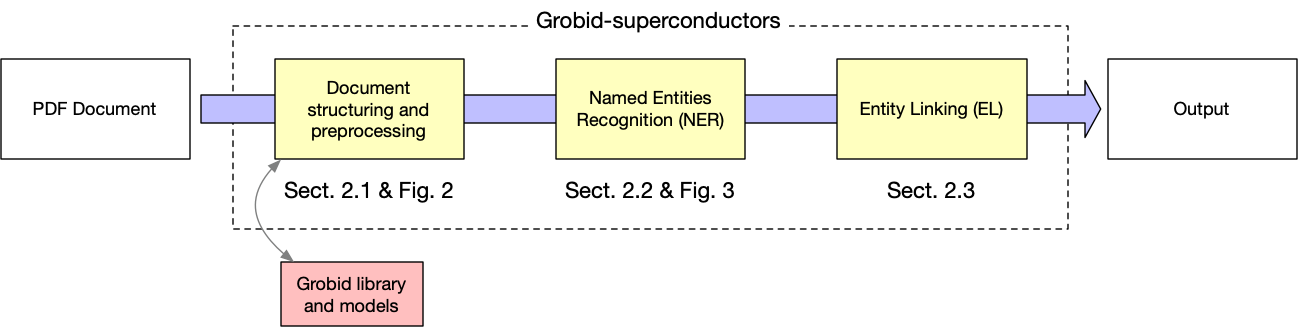
\includegraphics[width=\textwidth]{figures/automatic_extraction_supercon/schema-architecture-colors.png}
    \caption{Processing pipeline for extracting superconductors materials and properties. }
    \label{fig:pipeline-overview}
\end{figure}

\paragraph*{Abstract versus full-text}
At the time of writing this paper, we are aware of related works that utilise text from abstracts as training data for machine learning.
The main reason for using abstracts is that they are usually freely available as text~\cite{kononova2019text}, and contain condensed information~\cite{yamaguchi-etal-2020-sc, court2020magnetic}.
Accurately parsing the full-text presents more challenges, however, but they are mitigated by Grobid and, the full-text contain a broader range of information, including the sample preparation process, negative results (e.g., absence of superconductivity for certain samples), and background information (e.g., reports on other materials from referenced works).
% Such examples are needed to supply knowledge of non-superconductivity when building a superconductors prediction model~\cite{stanev_machine_2017}. 
Thus, grobid-superconductors is built to support full-text documents.

% Sentences vs Paragraphs 
\paragraph*{Paragraphs versus sentences}
Another question related to natural language processing (NLP) is whether to use sentence-based or paragraph-based text.
While paragraphs can be extracted as part of the layout of PDF documents, obtaining sentences adds an additional step in which text is processed with a sentence segmenter.
However, sentences are almost always shorter by definition, and in deep learning, this has advantages.
In training and prediction, sentences will likely be shorter than the ``max sequence length'' limitation (e.g., 512 tokens for transformers).
During training, sentences also use less memory and allow us to train models with a larger ``batch size'', which has been shown to improve efficiency and obtain better results~\cite{liu2019roberta}. 


\begin{table}[ht]
    \centering
    \caption{Results from cross-validation for sentence-based and paragraphs-based text.  }
    
    \begin{tabular}{lrrr}
        \toprule
        \textbf{Label}             & \textbf{Precision} & \textbf{Recall} & \textbf{F1} \\
        \midrule
        Paragraph-based micro avg. & 44.44              & 27.21           & 33.76       \\
        Sentence-based micro avg.  & 48.41              & 50.00           & 51.70       \\
        \bottomrule
    \end{tabular}

    \label{tab:comparison-evaluation-sentences-paragraphs}
\end{table}

We chose to use sentence-based text in Grobid-superconductors after performing preliminary experiments on our tasks typologies, but on a smaller scale. 
For the Named Entities Recognition (NER) task we trained and evaluated a sequence labelling model for each version (paragraph-based and sentence-based) on four annotated documents (3/1 document partition for training/evaluation) from SuperMat~\cite{foppiano2021supermat}.
As indicated in Table~\ref{tab:comparison-evaluation-sentences-paragraphs}, the F1-score increased by 17.94 percentage points when the sentence-based text was used.
% Our intuition suggests that this improvement can be mainly explained by the increase in the number of training examples for the same amount of text.

For the Entity Linking (EL) task, we want to maximise precision. 
In our previous work~\cite{foppiano2019proposal} we noticed that limiting linking entities within the same sentence (versus paragraph) would obtain higher precision (68.7\% versus 57\%) at the expense of lower recall (6.5\% versus 10.7\%), and F1-score (11.87\% versus 18.01\%).
Therefore, in both our tasks we found evidence that a sentence-based dataset is more beneficial than paragraph-based dataset.


\section{Document structuring and pre-processing}
\label{subsubsec:document-structuring}
In the first step of our process, the PDF document is converted into an internal model based on a list of text statements, tokens, and features.
The input document is processed using the Grobid original models, where we apply customised processes for document header and content.
We select a subset of bibliographic information from the header: title, authors, DOI, publisher, journal, and year of publication, and we consolidate them via Grobid to match the publisher's quality (even by processing the ``preprint version'' of the publication).
The superconductors entities extraction is applied to the content, only on relevant text items: title, abstract, text content from body or annexes, text content from figure and table captions (Figure~\ref{fig:grobid-document-processing}).

\begin{figure}[ht]
    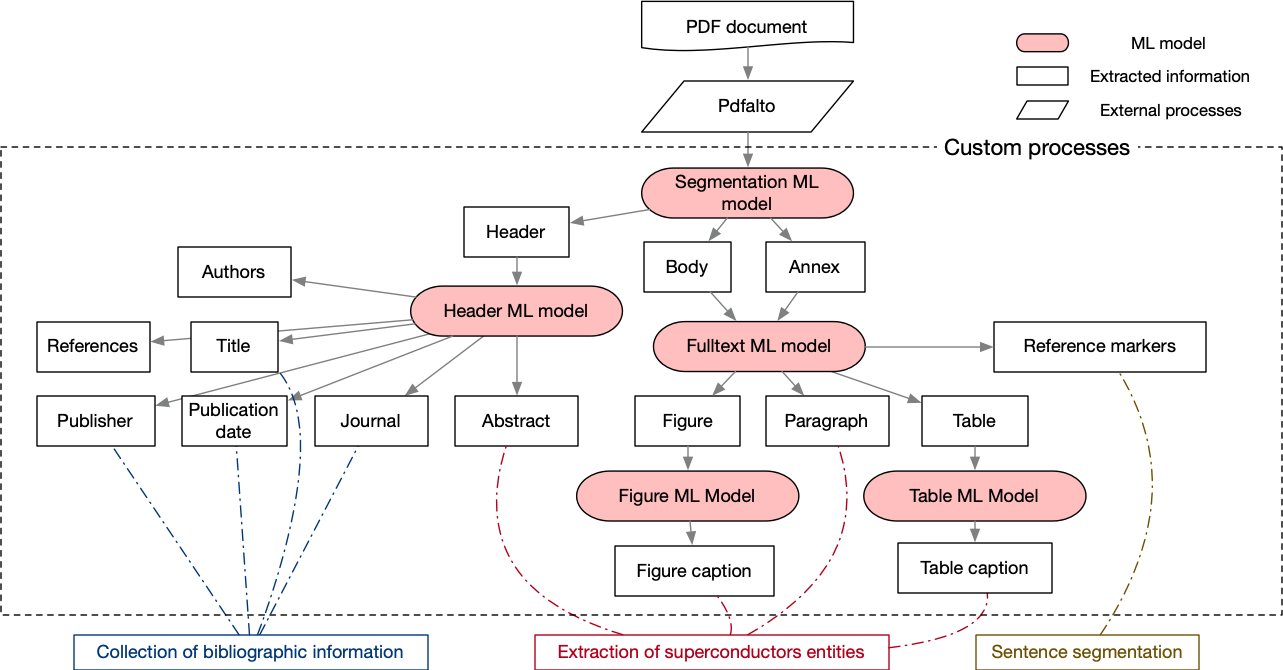
\includegraphics[width=\textwidth]{figures/automatic_extraction_supercon/document-structuring-colors}
    \caption{Grobid-superconductors extraction processes (bibliographic information, superconductor entity extraction and sentence segmentation) within the Grobid cascade data flow.}
    \label{fig:grobid-document-processing}
\end{figure}

We use the collected reference markers (also called \textit{reference callouts}) from the text as features for improving the paragraph segmentation in sentences: the segmentation is cancelled if the end of sentence falls within the boundaries of a reference marker.
For example, a sentence containing a reference in the form ``Foppiano et. al.'' may be mistakenly segmented in the middle at the token ``et.''.

% The main properties are: 
% \begin{itemize}
%     \item \textit{LayoutTokens} stores the layout information of each token: style (italic, bold, superscript, and subscript), font (font type, font size), positions (coordinates (a list of pairs x,y), offset position), 
%     \item \textit{section} and \textit{subsection} are the Grobid main sections: header, body and annex, and the second-level processing (paragraph, table or figure caption, abstract, title), respectively,
%     \item \textit{spans} collects extracted entities including type, attributes (as key-value information), and offsets within text and layout tokens.
% \end{itemize}


\subsection{Named Entity Recognition}
\label{subsubsec:extraction}

In the second step, the Named Entity Recognition (NER) task is performed on the previously extracted text.

\subsubsection{Overview}

As illustrated in Figure~\ref{fig:extraction-ml-models-cascade-architecture} the ``superconductor parser'' extracts the main superconductor-related information by aggregating the resulting entities from two ML models.
The Superconductors ML model was developed based on the SuperMat schema~\cite{foppiano2021supermat}, and the Quantity ML model was developed in a separated Grobid module for measurement extraction~\cite{foppiano2019quantities} and the output is limited to only temperatures and pressures.
Overlapping entities are merged, exacted duplicates are removed, and the largest entities (in terms of string length) are preserved.
The resulting entities are summarised in Table~\ref{tab:superconductors-parser-entities}.

\begin{figure}[ht]
    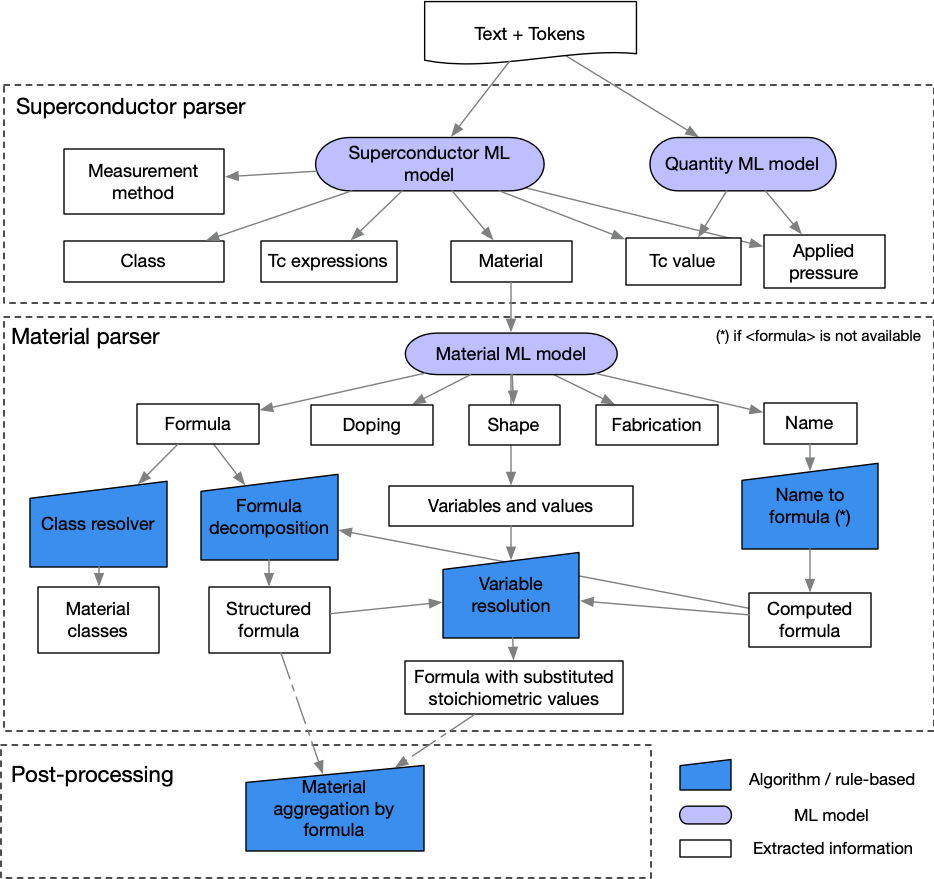
\includegraphics[width=\textwidth]{figures/automatic_extraction_supercon/schema-extraction-colors}
    \caption{\label{fig:extraction-ml-models-cascade-architecture} Cascade architecture in the NER step. The white rectangles indicate the extracted information (described in Tables~\ref{tab:superconductors-parser-entities} and~\ref{tab:material-parser-entities}).}
\end{figure}

\begin{table}[ht]
    \caption{Entities extracted by the superconductors parser.}
    \begin{tabular}{m{15em} m{20em}}
        \toprule
        \textbf{Entity} (\textbf{tag})              & \textbf{Description} \\
        \midrule
        Material (\texttt{<material>})              & Materials and samples names, formulas (including stochiometric formulas), substitution variables of values and elements, shape, doping, and substrate               \\
        Class (\texttt{<class>})                    & Groups of materials having similar characteristics or common strategic compounds that define their nature                                                      \\
        \tc value (\texttt{<tcValue>})      & The value of the superconductor critical temperature                                                                                                          \\
        \tc expressions (\texttt{<tc>})     & Expressions in the text that provide information about the phenomenon of superconductivity related to a value, interval or variation of the \tc \\
        Measurement method (\texttt{<me\_method>}) & Technique used to measure or calculate the presence of superconductivity                                                                                     \\
        Applied pressure (\texttt{<pressure>})      & Applied pressure when superconductivity is recorded                                                                                                            \\
        \bottomrule
    \end{tabular}
    \label{tab:superconductors-parser-entities}
\end{table}

Entities of type \texttt{<material>}, which may contain mixed heterogeneous information, are passed in the cascade to the ``Material parser'' which aggregates ML and other tools.
First, the entity is passed through a Material ML model to segment and identify its content (Table~\ref{tab:material-parser-entities}).
Then, different processes are applied, depending on which information is available. 
These processes include the following:
\begin{itemize}
    \item Formulas are decomposed into a structured composition. We identify each element-stoichiometry pair (e.g., ``O'': 7.0) using mat2chem~\cite{kononova2019text} and Pymatgen~\cite{Ong2013}; if only the material name is available, we lookup its formula (e.g., hydrogen to \textit{H}),
    \item Using heuristics, we classify the formula by assigning multiple classes as they are understood from superconductor researchers, for example cuprate, oxides, alloys, etc.
    \item Using the variables and values extracted, we substitute them into partial formulas. For example, in \texttt{La 4 Fe 2 A 1-x O 7 (A=Mg,Co; x=0.1,0.2)}, we substitute \textit{A} and \textit{x} using their parsed values, and applying permutations, we obtain four \textit{resolved formulas}: \texttt{La 4 Fe 2 Mg 0.9 O 7}, \texttt{La 4 Fe 2 Mg 0.8 O 7}, \texttt{La 4 Fe 2 Co 0.9 O 7}, and \texttt{La 4 Fe 2 Co 0.8 O 7}.
\end{itemize}

\begin{table}[ht]
    \caption{Entities extracted by the material parser. }

    \begin{tabular}{m{16em} m{30em}}
        \toprule
        \textbf{Entity} (\textbf{tag})               & \textbf{Description}                                                                                                              \\
        \midrule
        Name (\texttt{<name>})                       & The canonical name of a material (e.g., hydrogen, PCCO, carbon)                                                                    \\
        Formula (\texttt{<formula>})                 & Chemical formula of the material (e.g., \texttt{Pr1.869Ce0.131CuO 4-}, \texttt{MgB2}, \texttt{La 2-x Sr x CuO 4})                  \\
        Doping (\texttt{<doping>})                   & Doping ratio and doping materials that are adjoined to the material name (e.g., \texttt{Zn-doped}, \texttt{2\% Zn-doped})          \\
        Shape (\texttt{<shape>})                     & shape of the material (e.g. single crystal, polycrystalline, thin film, powder, film)                                             \\
        Substitution variables (\texttt{<variable>}) & Variables that can be substituted in the formula.                                                                                 \\
        Substitution values (\texttt{<value>})       & Values expressed in the doping.                                                                                                   \\
        Substrate (\texttt{<substrate>})             & Substrates as defined in the material name                                                                                        \\
        Fabrication (\texttt{<fabrication>})         & Additional information that does not belong to any of the previous tags  (e.g., intercalated, electron-doped) \\
        \bottomrule
    \end{tabular}
    
    \label{tab:material-parser-entities}
\end{table}

Finally, after all entities are extracted, the post-processing aggregates different mentions of the same materials using the parsed formulas at the document-level.
For example, formula with partial substitutions such as \texttt{La 2 Fe 1-x O 7 (x = 0.1, 0.2)} will be aggregated with materials like \texttt{La 2 Fe 0.9 O 7} appearing in other sections of the same document.

\subsubsection{Machine Learning study}

In this section we discuss the novel ML models we have trained for extracting specialised entities: the Superconductor ML model and the Material ML model (Figure~\ref{fig:extraction-ml-models-cascade-architecture}).
SuperMat~\cite{foppiano2021supermat}, our training dataset, contains 164 papers as of the time of writing and is composed of annotated full-text and layout features from PDF documents.

For both ML models we trained and evaluated the following four architecture/implementations: linear CRF (CRF), bidirectional LSTM with CRF~\cite{Lample2016NeuralAF} (BidLSTM\_CRF), bidirectional LSTM with CRF with Features~\cite{Lample2016NeuralAF} (the same as (BidLSTM\_CRF) with an additional input channel for features; BidLSTM\_CRF\_FEATURES), and SciBERT~\cite{Beltagy2019SciBERT} using a CRF as the activation layer (Scibert).

The ML models are interfaced by Grobid, which uses the Wapiti\cite{lavergne2010practical} implementation for linear CRF, and DeLFT (Deep Learning For Text)~\cite{DeLFT} for deep learning models.
The architectures CRF and BidLSTM\_CRF\_FEATURES make use of the orthogonal features we have summarised in Table~\ref{tab:ML-model-features}.

\paragraph*{Superconductor ML model}

\subparagraph*{Holdout set}
The holdout set evaluation consists in using a fixed part of a dataset for validation. 
The selection must be performed to reproduce the same distribution of entities of the original dataset.
We assembled the holdout set by manually selecting 32 documents (24\%) from SuperMat, making sure they had a similar ratio of examples, entities and unique entities with the remaining 76\% (132 documents) which was used as training set (Figure~\ref{fig:training-holdout-set-distribution}a).
Maintaining the same rate for entity type distribution between the two sets was more challenging: on average, we obtained about 15-18\% of labels of each type in the holdout set (Figure~\ref{fig:training-holdout-set-distribution}b), except for the \texttt{<material>} label (23\%). %(Tables~\ref{tab:training-holdout-set-distribution-annex} and \ref{tab:training-holdout-distribution-labels}). 
%The remaining 76\% (132 documents) is used for training.


\begin{figure}[ht]
    \centering
    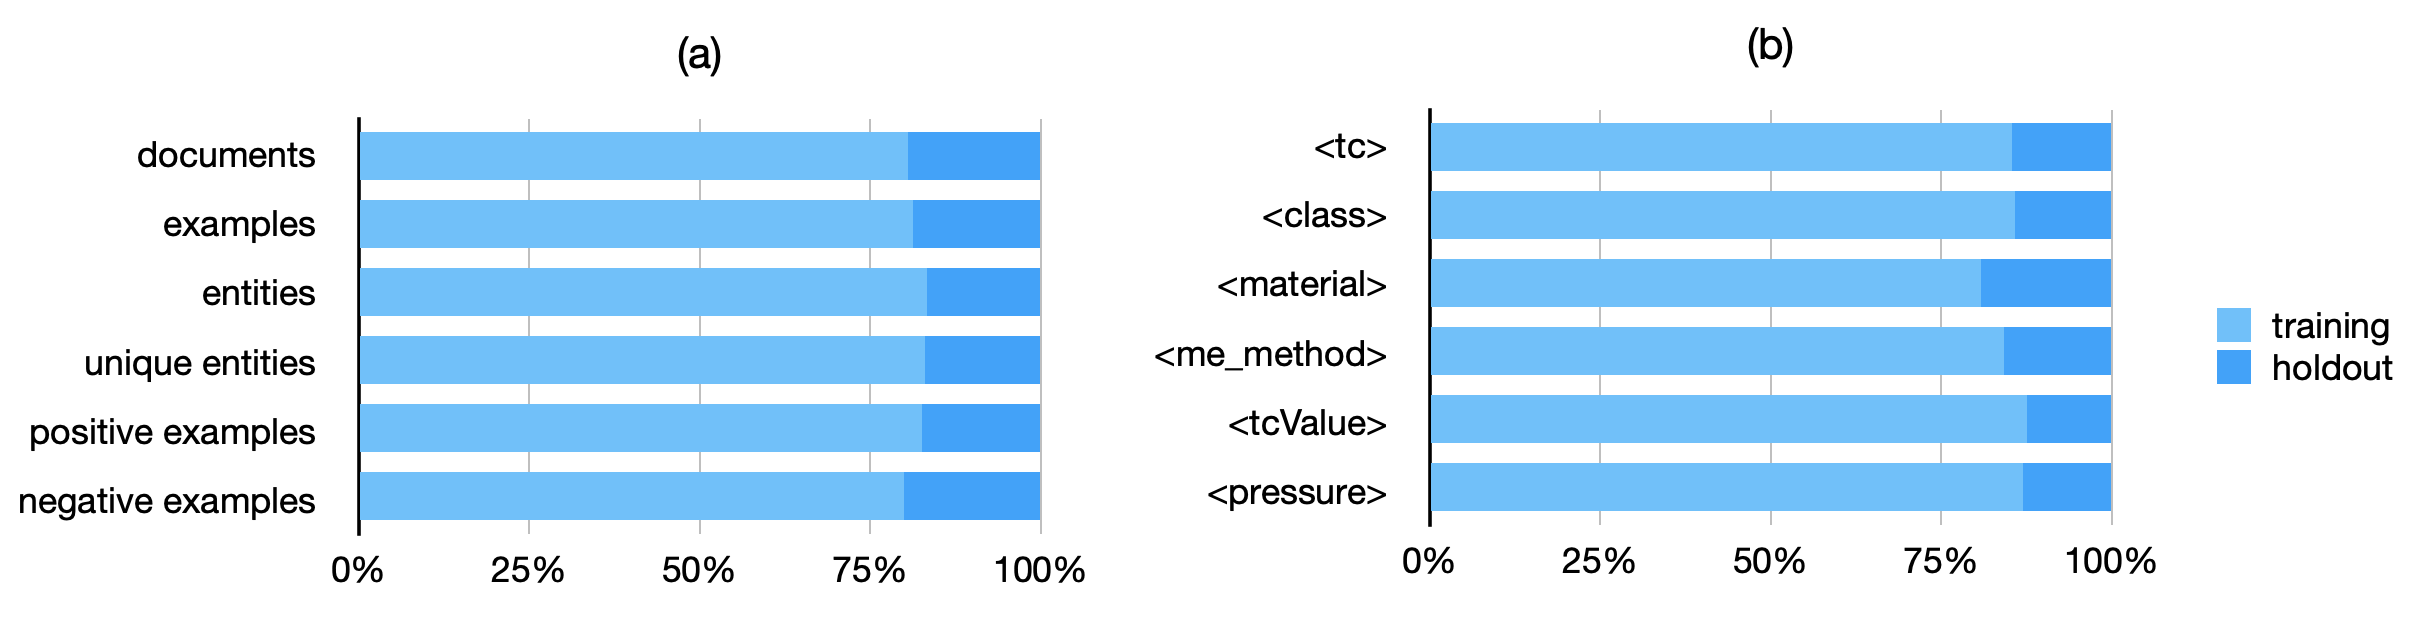
\includegraphics[width=\textwidth]{figures/automatic_extraction_supercon/superconductor-holdout-training-set}
    \caption{Holdout/training set distribution for (a) general metrics and (b) entity labels; entities and unique entities indicate the number of labelled entities with and without value duplicates, respectively, and positive examples (+) and negative examples (-) indicate the number of sentences with at least one entity and with no entities, respectively.}
    \label{fig:training-holdout-set-distribution}
\end{figure}

\begin{figure}[ht]
    \centering
    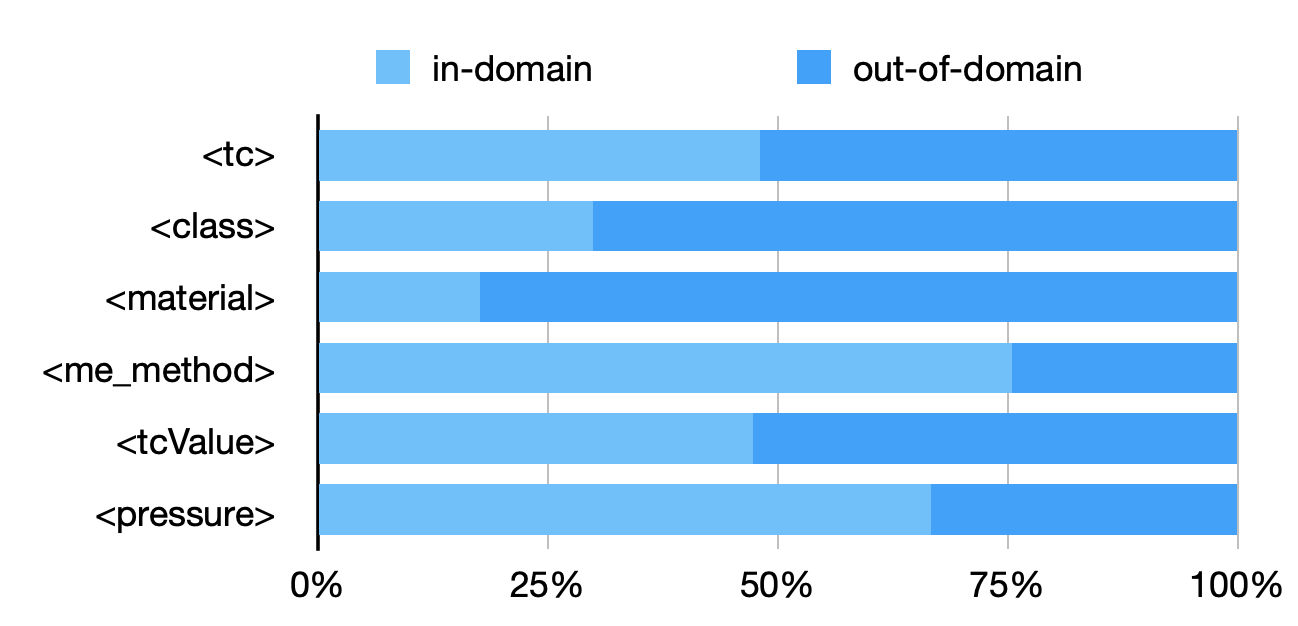
\includegraphics[width=0.6\textwidth]{figures/automatic_extraction_supercon/superconductor-out-domain-holdout-unique}
    \caption{Holdout ``out-of-domain'' rates. The entities from the holdout set that are also in the training set are ``in-domain'' and the entities that are not in the training set are ``out-of-domain''.}
    \label{fig:out-domain-holdout}
\end{figure}

We defined the ``out-of-domain'' ratio as the number of unique entities from the holdout set that were not in the training set.
The holdout set ``out-of-domain'' ratio was on average around 72\%, which challenge the model generalisation (every 100 entities in the holdout set, 72 were never seen before during training).
Most of the labels had an ``out-of-domain'' ratio above 50\%  (Figure~\ref{fig:out-domain-holdout});  \texttt{<material>}, the most important label, had the highest ratio (82\%) while \texttt{<me\_method>} and \texttt{<pressure>} have the lowest (25\% and 33\%). 
The low ratio of \texttt{<me\_method>} can be explained by their low entity variability (11.44\%).

\subparagraph*{Positive sampling}
We trained the model with positive sampling by removing the examples without entities (negative examples, Figure~\ref{fig:training-holdout-set-distribution}a).
This approach provided an improvement of 2\% in both precision and recall as compared to the result without sampling when testing against the holdout set.
Additional experiments with active and random sampling~\cite{lopez2021mining} with ratios of negative examples of 0.1, 0.25, 0.5 and 1.0 did not provide stable evidence suggesting scoring improvements when testing against the holdout set. 

\subparagraph*{Evaluation}
The best results were obtained by Scibert with an F1 of 77.03\% and a recall of around 80.69\% (Table~\ref{tab:evaluation-superconductors-ML-model}).
The features did not provide any improvements with RNN models: BidLSTM\_CRF and BidLSTM\_CRF\_FEATURES resulted in the same F1 score.
This result comes as a surprise because features such as superscript/subscript were expected to be determinants for recognising material sequences.


\begin{table}[ht]
    % \centering\small
    \caption{Evaluation scores (\%) for the Superconductor ML model in the four architectures. For the DL architecture the results are averaged over 5 runs. Support (Supp) indicates the number of labels in the training data. Values in bold indicate the highest score. P: precision, R: recall.}
    
    \scalebox{0.8}{
        \begin{tabular}{l ccc ccc ccc ccc r}
            \toprule
            \textbf{Label}        & \SetCell[c=3]{c}{\textbf{CRF}} & \SetCell[c=3]{c}{\textbf{BidLSTM\_CRF}} & \SetCell[c=3]{c}{\makecell{\textbf{BidLSTM\_CRF}                                                                                                                                                 \\\textbf{\_FEATURES}}} & \SetCell[c=3]{c}{\textbf{Scibert}} & \textbf{Supp} \\
            \cmidrule(lr){2-4}\cmidrule(lr){5-7}\cmidrule(lr){8-10}\cmidrule(lr){11-13}\cmidrule(lr){14-14}
                                  & \textbf{P}                       & \textbf{R}                                & \textbf{F1}                                        & \textbf{P} & \textbf{R} & \textbf{F1}    & \textbf{P}     & \textbf{R} & \textbf{F1}    & \textbf{P} & \textbf{R}     & \textbf{F1}    &      \\
            \midrule
            \texttt{<class>}      & 79.74                            & 66.79                                     & 72.69                                              & 79.01      & 72.62      & \textbf{75.66} & 77.84          & 72.40      & 74.97          & 72.95      & 75.28          & 74.09          & 1646 \\
            \texttt{<material>}   & 79                               & 72.15                                     & 75.42                                              & 79.25      & 76.94      & 78.06          & 81.07          & 75.10      & 77.94          & 80.15      & 81.42          & \textbf{80.77} & 6943 \\
            \texttt{<me\_method>} & 60.25                            & 68.73                                     & 64.21                                              & 56.41      & 79.49      & 65.92          & 55.86          & 80.45      & 65.90          & 56.26      & 81.52          & \textbf{66.56} & 1883 \\
            \texttt{<pressure>}   & 46.15                            & 29.27                                     & 35.82                                              & 49.45      & 58.05      & 52.53          & 50.25          & 60.49      & \textbf{54.36} & 41.72      & 52.68          & 46.51          & 274  \\
            \texttt{<tc>}         & 84.36                            & 83.57                                     & \textbf{83.96}                                     & 78.61      & 82.54      & 80.48          & 79.19          & 82.07      & 80.60          & 74.46      & 82.66          & 78.35          & 3741 \\
            \texttt{<tcValue>}    & 69.8                             & 66.24                                     & 67.97                                              & 70.36      & 75.16      & 72.67          & 68.95          & 76.56      & 72.52          & 70.90      & 79.74          & \textbf{75.06} & 1099 \\
            \midrule
            All (micro avg)       & 76.88                            & 72.77                                     & 74.77                                              & 74.59      & 77.67      & 76.09          & \textbf{75.17} & 76.79      & 75.96          & 73.69      & \textbf{80.69} & \textbf{77.03}        \\
            \bottomrule
        \end{tabular}
    }
    
    \label{tab:evaluation-superconductors-ML-model} 
\end{table}

The \texttt{<pressure>} label had the lowest performance scores in all architectures. We believe that 274 training examples are not a sufficient large number considering that pressure expressions can be dependent on the context because they can refer to different types of pressures (e.g., annealing pressure).
The label with the highest score was \texttt{<material>}, with F1 values of 80.77\% and 78.06\% for Scibert and BidLSTM\_CRF, respectively. In addition, \texttt{<material>} had the highest ``out-of-domain'' ratio in the holdout set (greater than 75\%, Figure~\ref{fig:out-domain-holdout}) and the highest ``label variability'' (the ratio between unique entities and total entities, about 42\%), which suggests that the model recognises correctly materials that has not been ``seen'' during the training.
On the other hand, the \texttt{<me\_method>} label, which has lower ``label variability'' (around 11\%) and a low ``out-of-domain'' ratio, had an F1 score of 66.56\% with Scibert and 65.92\% with BidLSTM\_CRF.
For \texttt{<tc>}, the CRF outperformed the other architectures (F1 score of 83.96\%), especially Scibert (78.35\%). 
This outcome can be explained by the extremely low variability (12.69\%) of entities labelled as \texttt{<tc>}. %, and having the holdout set with a balanced average ``out-of-domain'' ratio 51\%. 
% The entity labels variability (ratio of unique entities versus the total) is, in average, around 55\%, and 57\% for the training and holdout sets, respectively. \texttt{<tc>} (12\%) and \texttt{me\_method} have the lowest variability while the \texttt{<material>} has the highest. 

\begin{figure}[ht]
    \centering
    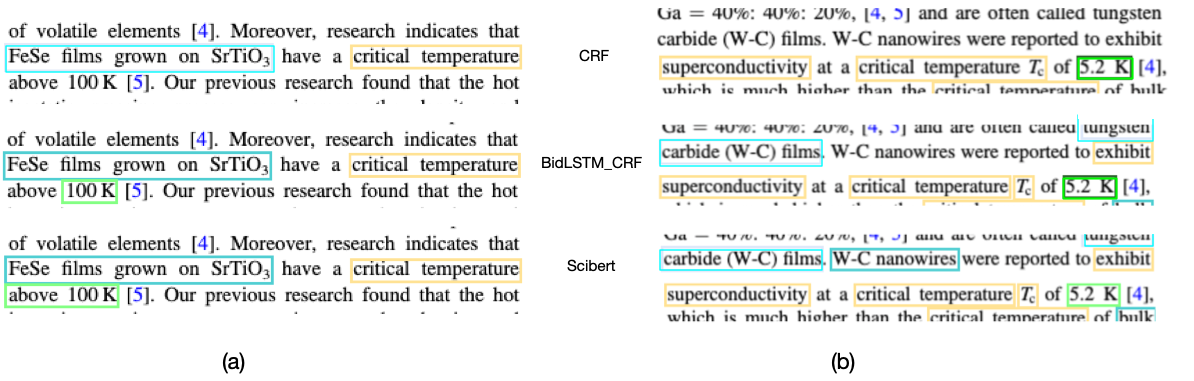
\includegraphics[width=\textwidth]{figures/automatic_extraction_supercon/example-comparison-archs.png}
    \caption{Examples taken from two sources~\cite{Gajda_2016, Shibata_2016} of results from three different architectures: CRF, BidLSTM\_CRF and, Scibert. The boxes annotating the text represent the extracted entities (material are indicated in light blue, \tc in green, and \tc expressions in yellow).}
    \label{fig:example-comparison-architectures}
\end{figure}

Scibert shows good generalisation capacity for unseen examples or examples appearing in different contexts.
For example, in Figure~\ref{fig:example-comparison-architectures}a, only Scibert correctly extracts ``above 100K'', while CRF misses it completely and BidLSTM\_CRF misses ``above''.
In the training data, ``above 100K'' is not present, but ``below 100K'' and ``\~100K'' are present, and several other entities contain the token ``above'' and Scibert can understand that the token ``above'' is relevant to the temperature.
In a second example (Figure~\ref{fig:example-comparison-architectures}b), only Scibert can correctly extract ``W-C nanowire'' which is not present in the SuperMat training data.
Unfortunately, we cannot check whether ``above 100K'' or ``W-C nanowire'' are also present in the dataset used in the pre-train of SciBERT by their authors~\cite{Beltagy2019SciBERT} because the data are not available.

\paragraph*{Material ML model}

To train the Material ML model we created a special dataset with an additional layer of labels (Table~\ref{tab:material-parser-entities}), which included the material information represented by entities annotated as \texttt{<material>} in the SuperMat documents.
% (label \texttt{<material>} from \textit{superconductors ML model}, Table~\ref{tab:superconductors-parser-entities}), that is,

\begin{figure}[ht]
    \centering
    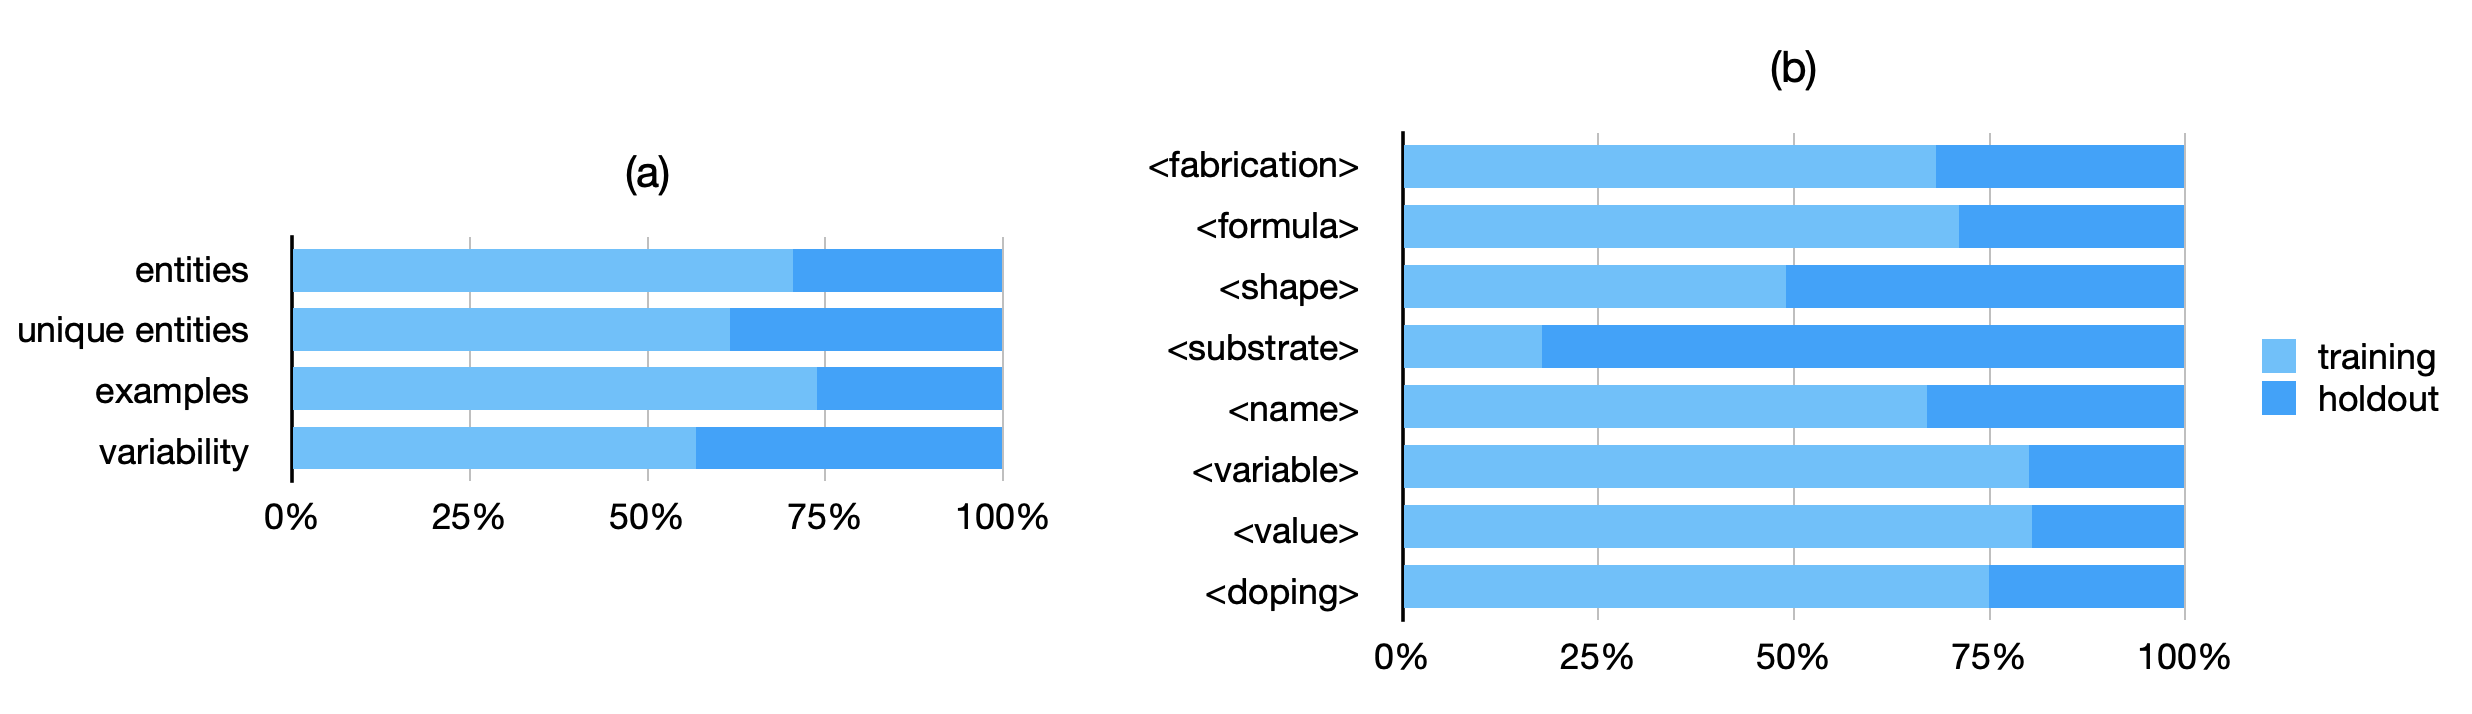
\includegraphics[width=\textwidth]{figures/automatic_extraction_supercon/material-holdout-training-set}
    \caption{Holdout/training set for the Material ML model: (a) general metrics and (b) entity labels.}
    \label{fig:material-training-holdout-set-distribution}
\end{figure}

\subparagraph*{Holdout set}
In this model we created an independent holdout set because the manual annotation work is performed on smaller chunks of text and requires less effort than annotating sentences as when we developed SuperMat.
We used material data extracted from a dataset of 500 documents (500-papers) from three publishers: \textit{American Institute of Physics} (AIP), \textit{American Physical Society} (APS) and \textit{Institute of Physics} (IOP)~\cite{foppiano2019proposal}.
The resulting holdout set has a average coverage greater than 25\% (Figure~\ref{fig:material-training-holdout-set-distribution}) and an average ``out-of-domain'' ratio of 83.93\% (Figure~\ref{fig:material-out-domain-holdout}).

\begin{figure}[ht]
    \centering
    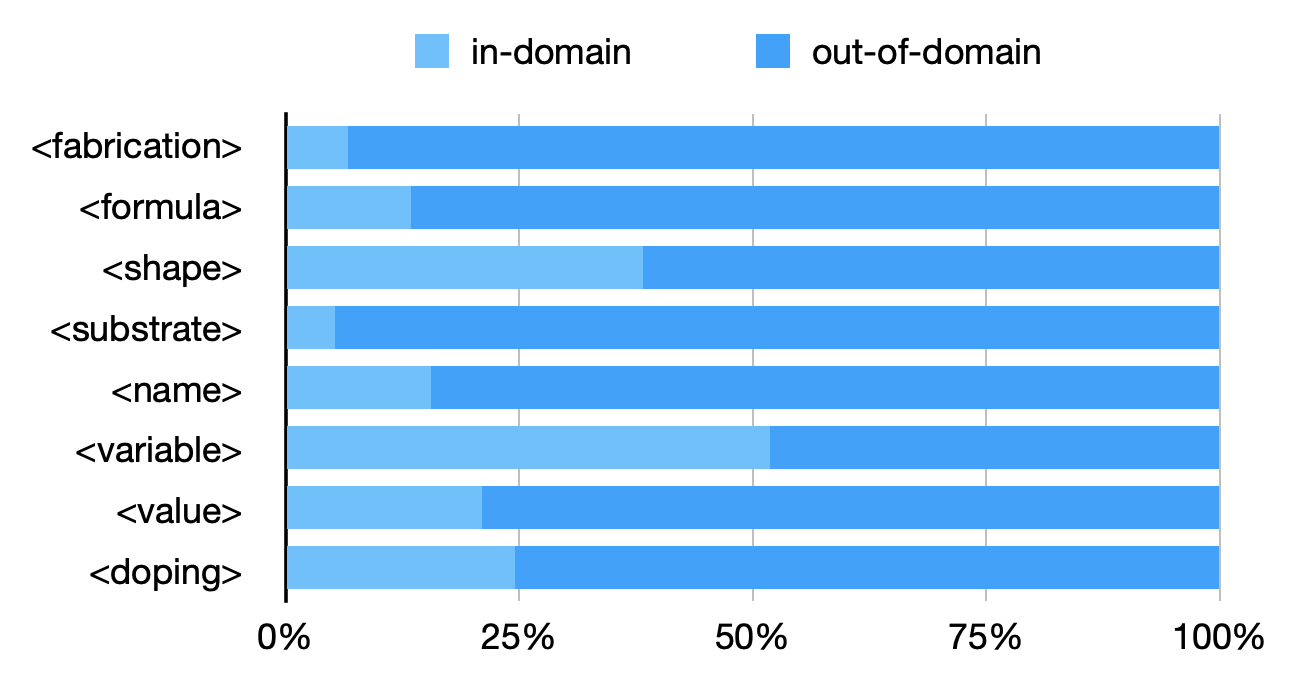
\includegraphics[width=0.6\textwidth]{figures/automatic_extraction_supercon/material-out-domain-holdout-unique}
    \caption{Holdout ``out-of-domain'' rates for the Material ML model. The entities from the holdout set that are also in the training set are the in-domain, and the entities that are not in the training set are the out-of-domain.}
    \label{fig:material-out-domain-holdout}
\end{figure}

\subparagraph*{Evaluation}

Scibert obtained the best results, with F1 at 84.15\% (Table~\ref{tab:evaluation-10fold-material-parser}).
The inclusion of features in the BidLSTM\_CRF architecture only improved results by less than 1\% (from 83.13 to 83.76\%).
The label \texttt{<fabrication>} did not perform well with any architecture, most likely because it is too generic (Table~\ref{tab:material-parser-entities}), and the content is too heterogeneous. Another label, \texttt{<substrate>} has only one-third of the training examples of \texttt{<fabrication>} but obtained results that were three times higher with Scibert, suggesting that \texttt{<fabrication>} should be split into separate and more homogeneous labels.

\begin{table}[ht]
    \centering\small
    \caption{Evaluation scores (\%) of the Material ML model with holdout set. Support (Supp) indicates the number of labels in the training data. Values in bold indicate the highest score. P: precision, R: recall.}
    
    \scalebox{0.8}{
    \begin{tabular}{l ccc ccc ccc ccc r}
        \toprule
        \textbf{Label}         & \SetCell[c=3]{c}{\textbf{CRF}} & \SetCell[c=3]{c}{\textbf{BidLSTM\_CRF}} & \SetCell[c=3]{c}{\makecell{\textbf{BidLSTM\_CRF}                                                                                                                                                 \\\textbf{\_FEATURES}}} & \SetCell[c=3]{c}{\textbf{SciBERT}} & \textbf{Supp}  \\
        \cmidrule(lr){2-4}\cmidrule(lr){5-7}\cmidrule(lr){8-10}\cmidrule(lr){11-13}\cmidrule(lr){14-14}
                               & \textbf{P}                       & \textbf{R}                                & \textbf{F1}                                        & \textbf{P} & \textbf{R} & \textbf{F1}    & \textbf{P}     & \textbf{R} & \textbf{F1}    & \textbf{P} & \textbf{R}     & \textbf{F1}    &      \\
        \midrule
        \texttt{<doping>}      & 60.41                            & 55.85                                     & 58.04                                              & 67.98      & 62.42      & 64.95          & 69.00          & 62.34      & \textbf{65.43} & 63.58      & 62.79          & 63.16          & 792  \\
        \texttt{<fabrication>} & 40.00                            & 4.55                                      & 8.16                                               & 23.61      & 5.91       & 9.24           & 37.33          & 9.09       & 14.48          & 22.51      & 13.18          & \textbf{16.52} & 94   \\
        \texttt{<formula>}     & 80.81                            & 82.29                                     & 81.54                                              & 82.59      & 84.14      & 83.35          & 83.83          & 85.14      & 84.47          & 84.53      & 86.56          & \textbf{85.53} & 6301 \\
        \texttt{<name>}        & 72.2                             & 63.75                                     & 67.71                                              & 76.29      & 78.76      & 77.43          & 74.51          & 80.38      & 77.33          & 77.18      & 81.86          & \textbf{79.44} & 1930 \\
        \texttt{<shape>}       & 90.89                            & 92.51                                     & 91.69                                              & 90.93      & 95.79      & \textbf{93.29} & 90.33          & 95.74      & 92.96          & 89.67      & 97.20          & 93.28          & 809  \\
        \texttt{<substrate>}   & 37.04                            & 6.76                                      & 11.43                                              & 54.31      & 32.43      & 40.44          & 60.08          & 33.38      & 42.82          & 56.32      & 41.22          & \textbf{47.59} & 32   \\
        \texttt{<value>}       & 80.21                            & 83.15                                     & 81.65                                              & 84.81      & 89.33      & 86.99          & 85.16          & 90.15      & \textbf{87.58} & 83.14      & 85.92          & 84.50          & 1895 \\
        \texttt{<variable>}    & 96.85                            & 95.98                                     & 96.41                                              & 95.19      & 97.77      & 96.46          & 96.32          & 97.90      & \textbf{97.10} & 96.22      & 96.52          & 96.37          & 1795 \\
        \midrule
        All (micro avg)        & 81.15                            & 78.09                                     & 79.59                                              & 82.76      & 83.50      & 83.13          & \textbf{83.20} & 84.33      & 83.76          & 83.11      & \textbf{85.23} & \textbf{84.15} &      \\
        \bottomrule
    \end{tabular}
}
    
    \label{tab:evaluation-10fold-material-parser}
\end{table}

\subsection{Entity Linking}
\label{subsubsec:linking}

%Introduction of the linking
Entity linking (EL) links materials and their corresponding properties.
%Objective of the linking
% We can formalised it as follows. \textit{Given a text T and two or more entities e\textsubscript{1}...e\textsubscript{n} of two types t\textsubscript{1} and t\textsubscript{2}, determine links between entities of type t\textsubscript{1} can be linked to entities of type t\textsubscript{2} .} 

%We have experimented several options: dependency parsing, rule-based, and sequence labelling. 
We use a rule-based algorithm, but there are other approaches such as the use of dependency parsing~\cite{yoshikawa:2017acl, Tiktinsky2020pyBARTES, swayamdipta:17, zhou-zhao-2019-head}. We did not use these because it was difficult to find a suitable dependency parser for scientific texts, and complementary methods based on complex rule sets were needed to compensate for the poor performance of the parser.

In our algorithm, pairs of entities are linked focusing on three types of link:
\begin{itemize}
    \item \textbf{material-tcValue}: The link between a material and its corresponding \tc.
    \item \textbf{tcValue-pressure}: The link between \tc and its related critical pressure.
    \item \textbf{me\_method-tcValue}: The link between \tc and its corresponding measurement method.
          % \item \textbf{material-crystal\_structure} link the material with their crystal structure, and 
          % \item \textbf{material-space\_group} to link the material to their space groups.
\end{itemize}

Entities of type \texttt{<tcValue>} are pre-processed through a classifier that establishes whether or not they temperatures related to the superconductivity. This is used to exclude other temperatures (e.g., annealing, transition, Curie) which might be incorrectly extracted by the previous step.
This rule-based classifier combines the extracted entities of \tc expressions (label \texttt{<tc>}) with a set of predefined standard terms.
If a temperature is not considered a \tc, it is excluded from the list of possible linking candidates.

Two scenarios are considered. First, if entities to be linked in the sentence are only two they are linked automatically, else further rules are applied. 
If the word ``respectively'' appears in the sentence, we apply ``order-linking''. 
For example, consider the following sentence:
\begin{displayquote}
    P-or Ba-122  and Co-doped Ba-122 have lower \tc's of about 30 K and 24 K, respectively, which makes helium free operation questionable.
\end{displayquote}
It contains the word ``respectively'', and by applying ``order-linking'', \textit{P-or Ba122} is assigned to \textit{30 K} and \textit{Co-doped Ba-122} to \textit{24 K}.
% Such method is very sensible to missing entities and we try to mitigate such scenario, knowing that nothing can be done when entities are missing in the middle of a sentence. 
% We ensure that missing entities at the boundaries limits the incorrect assignment by reducing the search space as follows: 
% \begin{itemize}
%     \item m entities of label\textsubscript{1} vs n entities of label\textsubscript{2} with $m > n$: we shift the starting point to start at the $m - $n entity
%     \item m entities of label\textsubscript{1} vs n entities of label\textsubscript{2} with $m < n$: we shift the ending point at the n\textsubscript{-1} entity
% \end{itemize}

% For example, the following sentence has three entities of type \texttt{<material>} and \texttt{<tcValue>}: 

If the word ``respectively'' does not appears in the sentence, we apply ``distance-linking'' which works by defining the distance measurement \textit{d} as a value calculated as the numbers of characters between the centroid of each entity.
Entities surrounded by parenthesis are expanded to the whole parenthesis, and its centroid is updated.
As an example, in the sentence
\begin{displayquote}
    We tested two materials MgB2 (Tc = 39 K) and FeSe (Tc = 16 K).
\end{displayquote}

\texttt{39 K} is closer to \texttt{FeSe} (\textit{d}=10) than to \texttt{MgB2} (\textit{d}=11). 
In this example, however, both temperatures entities would be expanded to their containing parenthesis (e.g. ``\texttt{39 K}'' to ``\texttt{(Tc = 39 K)}''. 
In this case the centre of the entity ``\texttt{39 K}'' is shifted toward the left, from the initial value of 38 to 35 and the distance from \texttt{MgB2} is reduced from \textit{d}=11 to \textit{d}=8.
As a result, the \texttt{MgB2} entity is correctly linked to ``\texttt{39 K}''.

The distance calculation is also adjusted with the addition of ``penalties'' by doubling the calculated distance when certain keywords or punctuations (``,'', ``.'', ``;'', ``and'', ``but', ``while', ``whereas', ``which'', ``although'') appear between two entities because they represent a logical separation of predicates ~\cite{oka2021table}.
In the above example, the distance between \texttt{39 K} and \texttt{FeSe} would be doubled (\textit{d}=20) and the link would not be made.


\begin{table}[ht]
    \centering
    \caption{Evaluation scores for the Linking. Support (Supp) indicates the number of labels in the training data. Values in bold indicate the highest score. P: precision, R: recall.}
    \begin{tabular}{lcccc}
        \toprule
        \textbf{Relationship type}          & \textbf{P} & \textbf{R} & \textbf{F1-} & Supp \\
        \midrule
        \textbf{material-tcValue}   & 88.40              & 74.52           & 80.87             & 726     \\
        \textbf{tcValue-pressure}   & 85.71              & 71.52           & 77.98             & 118     \\
        \textbf{me\_method-tcValue} & 62.28              & 65.74           & 63.96             & 151     \\
        \bottomrule
    \end{tabular}

    \label{table:evaluation-linking}
\end{table}


This rule-based linking was evaluated using the linked entities from SuperMat~\cite{foppiano2021supermat} (Table~\ref{table:evaluation-linking}) and is divided considering each link type.
The F1 score for the \texttt{material-tcValue} was about 80\% with a precision of 88.40\%. 
\texttt{tcValue-pressure} F1 score was 3\% lower than  \texttt{material-tcValue} considering much less data available (support was 118 compared with 726).

\subsection{End to end evaluation}

% What is the end 2 end evaluation? 
End-to-end evaluation (E2EE) measures the capacity of the system from the PDF documents until the final linked results.
We limited the scope of the E2EE to the triplet `material-\tc-pressure' which, at the moment, is the backbone upon which the database is built.
We performed the E2EE on the ``500-papers'' dataset where we manually examined the resulting database as follows: 1) we marked invalid records and 2) we identified the cause of failure from a predefined set of five \textit{error types} (Figure~\ref{fig:error-types}):
\begin{itemize}
    \item \textbf{From table}: the extracted text is wrongly extracted from a table. Although table content is ignored, the error rate from the Grobid library is still relevant due to the lack of training data.
    \item \textbf{Extraction}: entities are not recognised, wrongly recognised, or partially recognised.
    \item \textbf{Quantity extraction}: quantity entities (pressure, temperature) are not correctly extracted. We measured this error separately to identify the failure that could be shared with the Quantity ML model.
    \item \textbf{\tc classification}: the temperature is wrongly classified as superconducting \tc.
    \item \textbf{Linking}: given the initial steps were performed correctly, the resulting entities are not linked correctly.
\end{itemize}

\begin{figure}[ht]
    \centering
    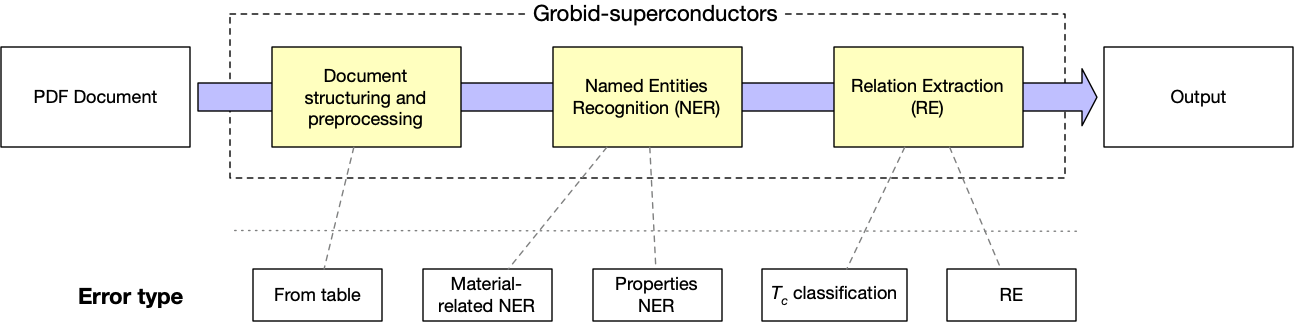
\includegraphics[width=\textwidth]{figures/automatic_extraction_supercon/error-types-colors}
    \caption{\textit{Error types} in the context of the data flow. }
    \label{fig:error-types}
\end{figure}

The E2EE scores are summarised in Table~\ref{table:end2end-evaluation-summary}.
Recall is omitted because it is less relevant and difficult to calculate manually.
The precision score (micro average) was 72.60\% for all the subsections, although the error rates of figure captions (59.28\%) and unknown subsections (57.14\%) were clearly lower than those of the other subsections ($>$ 70\%).
The `unknown` subsections indicate that the extracted text's structure was not well identified by Grobid but it was nevertheless aggregated.
The overall score increases to 73\% when excluding unknown subsections, 75.24\% when excluding figure captions, and 79.14\%  when excluding both.
Excluding these two subsections will not impact the amount of text, because both account for less than 20\% of the total number of subsections.

\begin{figure}[ht]
    \centering
    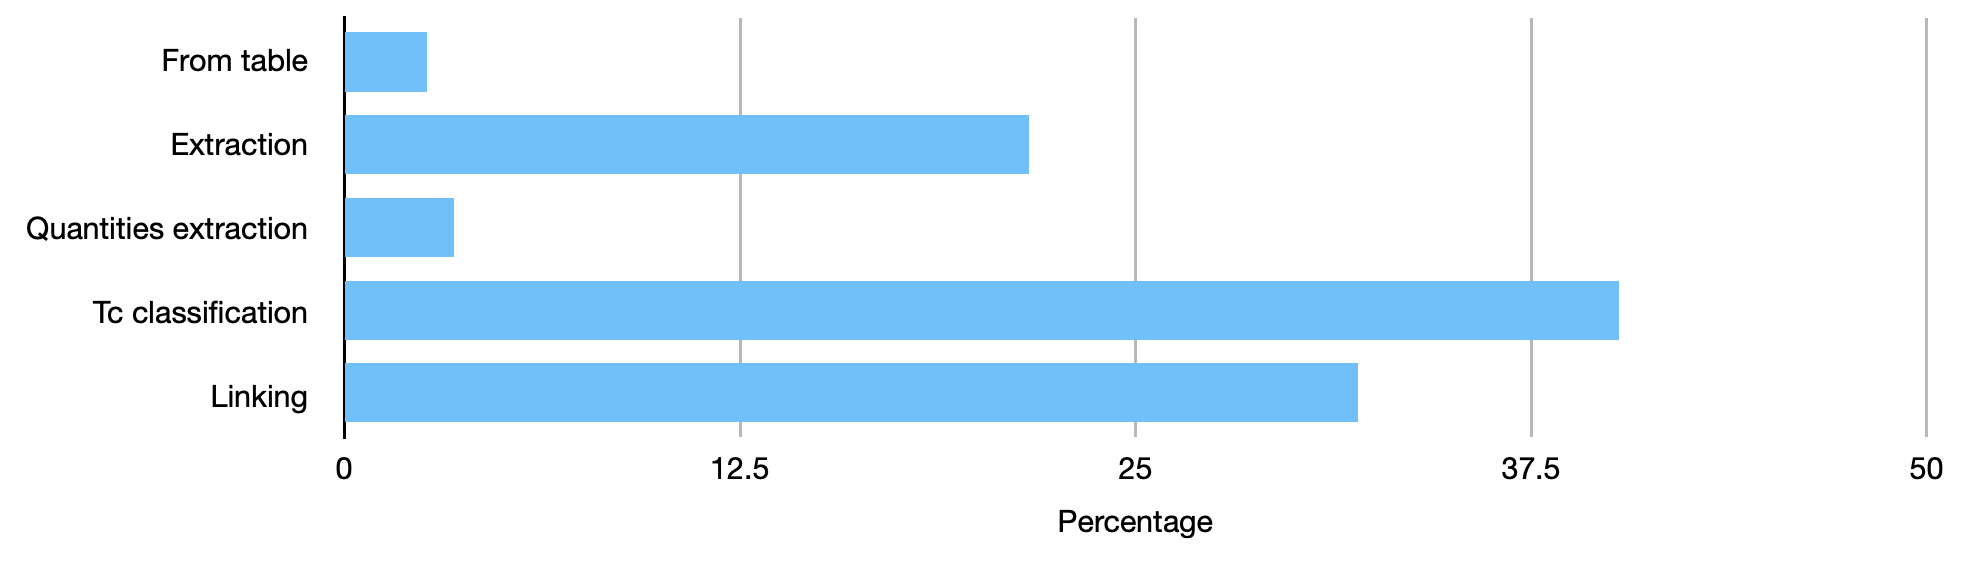
\includegraphics[width=\linewidth]{figures/automatic_extraction_supercon/error-types-bars-perc}
    \caption{Error type distribution in the E2EE of the \textit{500-papers} dataset.}
    \label{fig:error-types-distribution}
\end{figure}

The error types are summarised in Figure~\ref{fig:error-types-distribution}. The most common failures originate from \tc~classification (40\%), Linking (32\%), and Extraction (20\%).
The most common \tc classification failures are as incorrect recognition of 1) relative values of \tc (e.g., 1 K higher than material X); 2) values indicating the transition temperature width ($\Delta T_{c}$); 3) temperature values that are not \tc, for example, material synthesis temperatures ($T$), other critical transition temperatures that are not superconducting (e.g., $T_{Curie}$); and 4) values of temperature at which there is no superconductivity (e.g., ``at 70 K there is no superconductivity'').
``Linking errors'' mainly occur when the text compare relative values of \tc~using materials as the basis for comparison (e.g., ``The Tc = 38 K is similar to the one of MgB$_{2}$'').
Finally, ``Extraction'' issues mainly originate from: 1) implicit mention of the main material when experimented using different ``substrates'' combination, and 2) mismatches between \texttt{<material>} and \texttt{<class>} which, by definition, overlap.


\begin{table}[ht]
    \centering
    \caption{Summary of the E2EE evaluation scores. Support indicates the number of labels in the training data.}
    \begin{tabular}{l c c}
        \toprule
        \textbf{Subsection}                                      & \textbf{Precision} & \textbf{Support} \\
        \midrule
        Title                                                    & 100                & 2                \\
        Abstract                                                 & 80.32              & 61               \\
        Paragraph                                                & 75.2               & 623              \\
        Figure captions                                          & 59.28              & 140              \\
        Unknown                                                  & 57.14              & 21               \\
        \midrule
        \textbf{Micro avg.}                                      & 72.60              & 847              \\
        \textbf{Micro avg.} (excl. figures)                      & 75.24              & 707              \\
        \textbf{Micro avg.} (excl. unknown sections)             & 73.00              & 603              \\
        \textbf{Micro avg.} (excl. figures and unknown sections) & 79.14              & 657              \\
        \bottomrule
    \end{tabular}
    
    \label{table:end2end-evaluation-summary}
\end{table}


\section{Supercon\textsuperscript{2}}

We created SuperCon\textsuperscript{2} by processing 37770 research papers belonging to the category \textit{cond-mat.supr-cond} in ArXiv.
Currently SuperCon\textsuperscript{2} contains 40324 records including 2052 triplets with applied pressure (\textit{material-\tc-pressure}), and 3602 records with explicit measurement method (\textit{material-\tc-measurement method}).
The schema of SuperCon\textsuperscript{2} is summarised with examples in Table~\ref{tab:supercon2-schema}.

The data is processed and ingested through the asynchronous Map-Reduce approach~\cite{10.1145/1327452.1327492}.
The ``extraction task'' (Map) processes the PDF documents by accessing Grobid-superconductors via REST API and stores their processed representation together with the original PDF document.
Furthermore, the ``aggregation task'' (Reduce) reduces the document information into a synthesised tabular format.
We store the processed document representation in JSON format. 
The processed documents are kept separately and used for displaying the enhanced PDF document (Figure~\ref{fig:pdf-annotations}).
The pipeline uses a persistence layer for storage and reporting (logger).

\begin{figure}[ht]
    \centering
    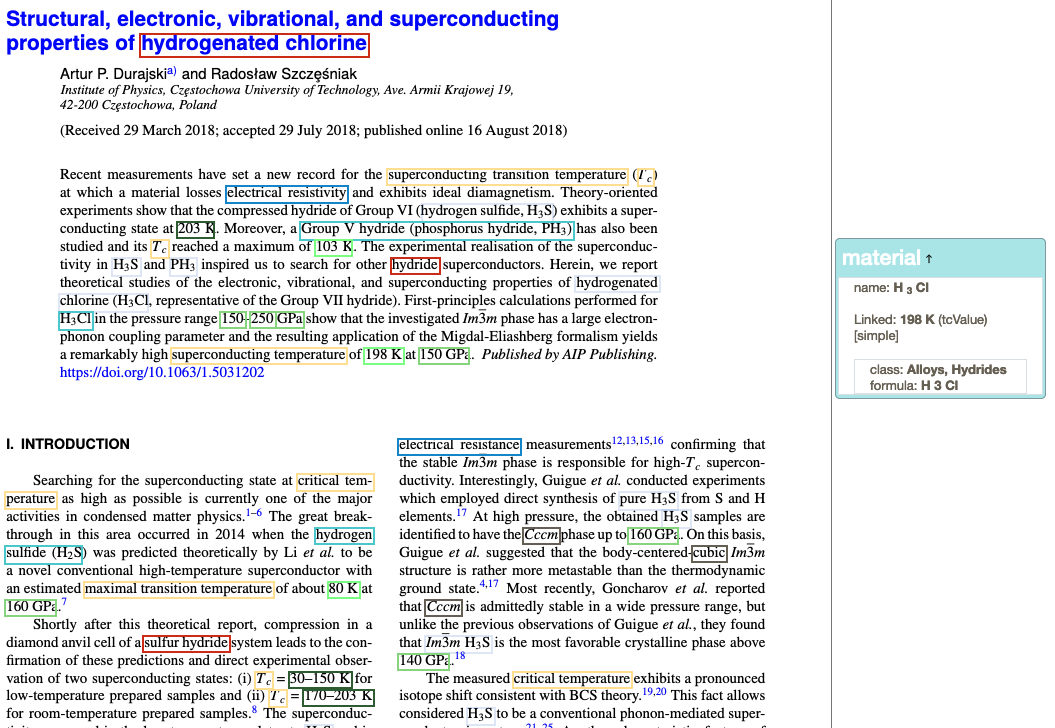
\includegraphics[width=0.8\textwidth]{figures/automatic_extraction_supercon/sample-pdf-annotations}
    \caption{\label{fig:pdf-annotations} Example of a superconductors research PDF document~\cite{sample_superconductors_article} enriched with extracted annotations. Materials information (class, formula) and properties (\tc) are summarised in the information box when the users click on the highlighted annotated entity in the text.}
\end{figure}



\afterpage {
    \clearpage % Flush earlier floats (otherwise order might not be correct)

    \begin{table}[ht]
        \centering
        \caption{Summary and description of the SuperCon\textsuperscript{2} schema. ``Internal information'' is technical information not accessible to the users.}
        % \scalebox{0.8}{
            \begin{tblr}{Q[l,m]Q[r,m]Q[r,m]}
                \hline[1pt]
                \textbf{Field name} & \textbf{Description}                             & \textbf{Examples}             \\
                \hline
                \SetCell[c=3]{c}{\emph{Material information}}                                                        \\
                \hline[dashed]
                {Raw                                                                                                   \\ material} & The material or sample as it appears in the text &\\
                \hline[dotted]
                Name                & Canonical name of a material                     & {PCCO, PCO, Metal diboride,   \\ hydrogen, carbon} \\
                \hline[dotted]
                Formula             & {Material expressed as chemical formula. This                                    \\ includes also formulas with stochiometric variables} & {$Pr_{1.869}Ce_{0.131}CuO_4-\delta$,\\ $MgB_2$, $La_{2-x} Sr_x CuO_4$} \\
                \hline[dotted]
                Doping              & {Doping ratio and doping materials                                               \\ that might be adjoined to the material} & {Overdoped, underdopded,\\ optimally doped,\\ bulk, pure, 1\% Zn, Zn\\ (from Zn-doped XYZ)}\\
                \hline[dotted]
                Shape               & The shape of the material or the sample          & {Single crystal, polycrystal, \\ wire, powder, film} \\
                \hline[dotted]
                Variables           & Variables that can be substituted in the formula & x = 0, RE=Ln,St               \\
                \hline[dotted]
                Class               & {Material classification according                                               \\ to the domain-experts taxonomy} & cuprates, oxides, and alloys\\
                \hline[dotted]
                Fabrication         & {All the information that does not                                               \\ belong to any of the previous tags} &  {Intercalated,\\ synthesized by MBE method,\\ electron-doped, hole-doped} \\
                \hline[dotted]
                Substrate           & Substrate material described in the raw material & {PCCO films onto              \\ $Pr_2 CuO_4 (PCO)/SrTiO_3$ }\\
                \hline[dashed]
                \SetCell[c=3]{c}{\emph{Properties}}                                                                  \\
                \hline[dashed]
                {Critical                                                                                              \\ Temperature}  & Superconducting critical temperature &\\
                \hline[dotted]
                {Applied                                                                                               \\ Pressure}  & {Pressure applied when measuring \\ the superconducting critical temperature} &\\
                \hline[dotted]
                {Measurement                                                                                           \\ Method}  & {Method for measurement of the\\ superconducting critical temperature} & {Magnetic susceptibility,\\ specific heat, calculation,\\ prediction, resistivity}\\
                \hline[dashed]
                \SetCell[c=3]{c}{\emph{Document bibliographic information}}                                          \\
                \hline[dashed]
                Section             & The main body section of the paper               & Header, body, annex           \\
                \hline[dotted]
                Subsection          & The secondary segmentation area of the paper     & {Paragraph, table caption,    \\ figure caption, title, abstract} \\
                \hline[dotted]
                {Authors,                                                                                              \\ Title, DOI,\\ Publisher,\\ Journal, Year} & \SetCell[c=2]{c}{Bibliographic information of the document}\\
                \hline[dashed]
                \SetCell[c=3]{c}{\emph{Internal information}}                                                        \\
                \hline[dashed]
                {Hash,                                                                                                 \\ Timestamp} & \SetCell[c=2]{c}{Hash calculated on the binary content of the original PDF\\ document and the timestamp when the document was processed.}\\
                \hline[1pt]
            \end{tblr}
        % }
        
        \label{tab:supercon2-schema}
    \end{table}
    \clearpage
}

\chapter{SuperMat: Construction of a linked annotated dataset from superconductors-related publications}
\label{cha:supermat}
% \section{Introduction}

\label{content-acquisition}
\section{Content acquisition}
SuperMat originates from PDF documents of scientific articles related to superconductor research. 
The PDF format is the most widely used format for scientific publications \cite{johnson2018pdfStatistics}.
The original documents were collected from the following sources: (a) the Open Access (OA) version of peer-reviewed articles referenced in the SuperCon database records; 
(b) articles provided by domain experts containing suitable items and potential links of material names, \textit{T\textsubscript{c}} values, measurement methods, and pressures; (c) articles from "condensed matter" category of arXiv (\url{https://arxiv.org/archive/cond-mat}) selected using the search terms of "superconductor", "critical temperature", and "superconductivity". 

Pre-print versions of peer-reviewed articles were obtained using a lookup service for bibliographic data called biblio-glutton (\url{https://github.com/kermitt2/biblio-glutton}) that aggregates data from various sources: the Crossref (\url{https://www.crossref.org/}) bibliographic database, the unPaywall (\url{http://unpaywall.org}) service, the PubMed Central repository (\url{https://pubmed.ncbi.nlm.nih.gov/}), and mappings to other databases. 
We queried \textit{biblio-glutton} using the bibliographic data of each article referenced in Supercon; subsequently, we downloaded the pre-print article associated with the retrieved record, if available. 
Although the published version may be different from the pre-print version of a document, the differences measured by comparing pre-print and peer-reviewed articles in biology~\cite{carneiro_comparing_2020} measured objective differences to be around 5\%.


\section{Preliminary annotation study}
\label{subsec:preliminary-annotation-study}
A preliminary annotation study was carried out to assess the effort required from the annotators to reach an acceptable Inter Annotation Agreement (IAA \textgreater 0.7) .
We annotated two randomly selected OA papers, by using a preliminary version of the guidelines with a limited tag-set of four labels: \texttt{<material>}, \texttt{<tc>} (expression describing the presence or absence of superconductivity), \texttt{<tcValue>} (value of \textit{T\textsubscript{c}}), and \texttt{<doping>} (amount of substitution, such as stochiometric values, usually expressed as functions of x or y).
The process was iterated multiple times.
Each iteration ended with computing the IAA using the Krippendorff's alpha coefficient~\cite{Krippendorff2004ReliabilityIC,Zapf2016MeasuringIR}, while annotators discussed the disagreements, and updated the guidelines.

\begin{table}[ht]
    \centering
    \caption{Summary of the IAA for each annotation iteration.}
    \begin{tabular}{ ccc } 
    \toprule
        \textbf{Iteration} \# & \textbf{IAA} & \textbf{IAA by label}  \\ [0.5ex] 
    \midrule
        1  & 0.45
        &\begin{tabular}{  cc  } 
            \texttt{<material>} & 0.45\\ 
            \texttt{<tc>} & 0.56\\
            \texttt{<tcValue>} & 0.50\\
            \texttt{<doping>} & 0.21\\
        \end{tabular}    
        \\ 
    \midrule
        2 & 0.65
        &\begin{tabular}{  cc  } 
            \texttt{<material>} & 0.75\\ 
            \texttt{<tc>} & 0.85\\
            \texttt{<tcValue>} & 0.85\\
            \texttt{<doping>} & 0.39 \\
        \end{tabular}          
        \\ 
    \midrule
        3 & 0.89
        & \begin{tabular}{  cc  } 
            \texttt{<material>} & 0.89\\ 
            \texttt{<tc>} & 0.91\\
            \texttt{<tcValue>} & 0.88\\
            \texttt{<doping>} & 0.94\\
        \end{tabular}       
        \\ 
    \bottomrule
    \end{tabular}
    
    \label{table:summary-preliminary-annotation}
\end{table}

Based on the results in Table~\ref{table:summary-preliminary-annotation}, IAA reached a satisfactory level around 0.9 after the third iteration. 
In the second iteration, although the average IAA reached 0.7 on three of the four labels, the average agreement was not satisfactory. 
When analysing the disagreement, we noticed that the low score in the \texttt{<doping>} label was caused by a heavy overlap with the \texttt{<material>} label, which required more precise definition in the guidelines. 

Based on this preliminary study, the following changes were implemented. 
(a) The label \texttt{<doping>} was merged under the \texttt{<material>} because, even with detailed documentation it was too difficult for humans to annotate them consistently.
(b) Three more labels were added: measurement methods and pressure (described as parametric conditions in relation to \textit{T\textsubscript{c}}), and class of materials. 

\subsection{Tag-set design}
The tag set (also referred to as \textit{labels}) represents the classes of entities and the type of links between them, which were designed to be extracted from the text (Figure~\ref{fig:example-annotations-and-links}).

% example-annotated-corpus-postprocess.png
\begin{figure}[ht]
  \centering
  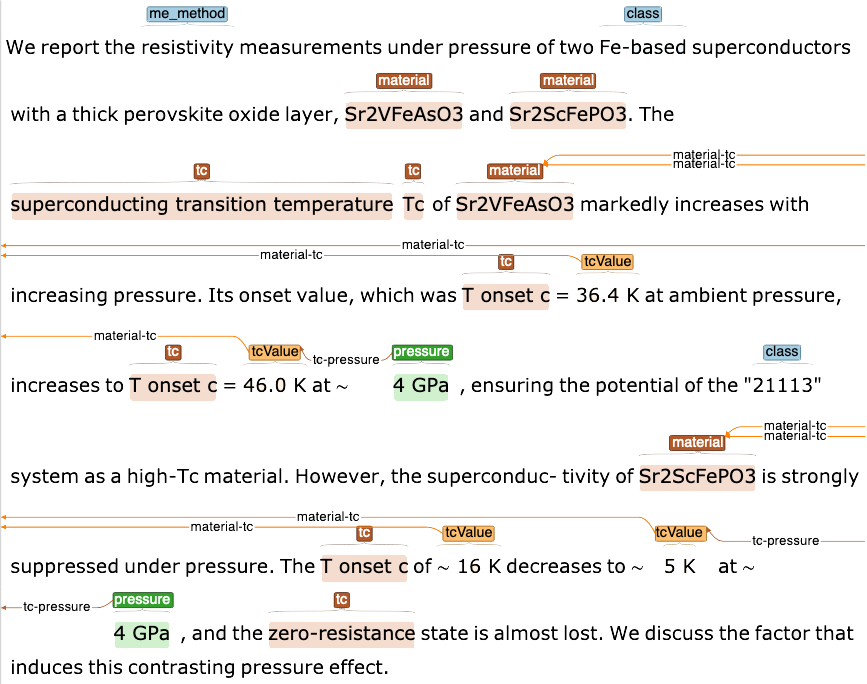
\includegraphics[width=\linewidth]{figures/supermat/Fig1.png}
  \caption{Example in the annotated corpus. Excerpt from © 2009 The Physical Society of Japan (J. Phys. Soc. Jpn. 78, 123707)}
  \label{fig:example-annotations-and-links}
\end{figure}


\subsubsection{Entities}
Entities (also referred to as Named Entities, mentions, or surface forms) are chunks of texts that represent information of interest, as follows: 

\begin{itemize}
\item Class (tag: \texttt{<class>}) represents a group of materials defined by certain characteristics.
Superconducting materials can be classified according to different criteria such as the composition and magnetic properties. 
Among publications collected for this study, the domain experts identified three types of classes based on: (a) the composition and crystal structure, (b) material phenomena (e.g. "I-type" and "II-type superconductivity", "BCS superconductors", "nematic", and "conventional/unconventional superconductivity"), and (c) high/low \textit{T\textsubscript{c}} value (e.g. "high-tc” superconductors). 

In this work, we only considered the (a) classes, mainly because the material composition and crystal structure do not change with time. For example, a cuprate from 1998 is still called a cuprate today. 
In comparison, many material phenomena used for (b) are not robust enough and can be biased by the viewpoint of the author(s) or research group, or the measurement methods. 
Finally, the definition of "high-tc" superconductors (c) is completely relative; i.e., with the progress of research, materials once considered "high-tc" might not be so anymore.

\item Material (tag: \texttt{<material>}) identifies the name of one or more materials. 
This label is used to collect the following types of information: 
\begin{itemize}
    \item Chemical formula indicating the material by its general or stochiometric formula (e.g. \texttt{LaFe\textsubscript{1-x}O\textsubscript{7}}, \texttt{WB\textsubscript{2}}),
    \item Compositional name (e.g. \texttt{magnesium diboride}) or abbreviations (e.g. \texttt{YBCO}), 
    \item The material's shape (e.g. wire, powder, thin film) or form of material (e.g. single/poly crystal), 
    \item Modification by a dopant (\texttt{Zn-doped}, \texttt{Si-doped}) or by percentage of doping (\texttt{2\%-doped}). We also considered qualitative expressions such as \textit{overdoped}, \textit{lightly doped}, and \textit{pure} as valid information, 
    \item Substrate information (e.g. \texttt{grown on MgO(100) film}) when it was adjacent to the material name or formula, in the text,
    \item Additional information about the sample (e.g. \texttt{as-grown}, \texttt{untwinned}, \texttt{single-layer}) when it was adjacent to the material name or formula, in the text. 
\end{itemize}

\item Superconducting critical temperature (tag: \texttt{<tc>}) identifies expressions related to the phenomenon of superconductivity. Any temperature mentioned in the text is not necessarily the \textit{T\textsubscript{c}}. Rather, it could refer to the temperature for other processes/events such as annealing/sintering temperature, specific measurements, and structural changes.
This label identifies the presence or absence of superconductivity at a given temperature.
In addition, modifiers of this information (increasing/decreasing \textit{T\textsubscript{c}}) are also retained. 

\item Superconducting critical temperature value (tag: \texttt{<tcValue>}) represents the temperature at which the superconducting phenomenon occurs. 
It can be defined by different experimental criteria, such as the onset, mid-point of resistivity drop, or zero resistivity.
This value also considers boundary conditions, such as the \textit{onset of superconductivity}, \textit{zero resistance}. 

\item Applied pressure (tag: \texttt{<pressure>}) indicates the applied pressure corresponding to a measured \textit{T\textsubscript{c}}. 

\item The measurement method (tag: \texttt{<me\_method>}) indicates the method used to measure or calculate the presence of superconductivity. Here, we considered the following categories: resistivity, magnetic susceptibility, specific heat, and theoretical calculations. 
\end{itemize}

\subsubsection{Links}
The links connect entities of materials or samples to their corresponding properties, conditions, and results. 
The links are non-directional, and there are no restrictions on the number of links for each entity. 
We defined three types of links:

\begin{itemize}
    \item material-tc: linking materials to their \textit{T\textsubscript{c}} values.
    \item tc-pressure: connecting \textit{T\textsubscript{c}} and the applied pressure under which it was obtained.
    \item tc-me\_method: linking \textit{T\textsubscript{c}} and the corresponding measurement method. 
\end{itemize}


\subsection{Annotation guidelines}
\label{subsec:annotation-guidelines}
Annotation guidelines include the principles and the rules that describe what constitutes as desired information for the SuperMat dataset and how to annotate it. They include detailed descriptions of the specific rules that have been defined for each type of information to be annotated, with one or more definitions and examples illustrating what to annotate in different cases, exceptions, and references. We used an online system to track the discussions and decisions when a question or a comment was raised and provided a link to such issues in the respective description or example. 
In addition, the guidelines include \textit{linking rules} that provide information on how to correctly connect the entities in a relationship. 
The guidelines were built using a dynamic markup language (called RestructuredText) and stored in a git (\url{https://git-scm.com/}) version control system repository. We deployed them as HTML files via web, which were updated automatically after each modification. They can be accessed at \url{https://supermat.readthedocs.io}.

\subsection{Annotation support tools}
\label{subsec:annotation-support-tool}
The task of annotating documents is tedious and requires both attention and subject knowledge from the annotators.
Annotation support tools aim to maximise the efficiency of annotators and minimise human mistakes. 
They are composed of a web-based collaborative annotation tool, automatic annotation suggestions, and automatic corpus analysis. 

\subsubsection{Web-based collaborative annotation tool: INCEpTION}
\label{subsec:annotation-tool}

The annotation tool is the platform used for creating, correcting and linking annotations.
After evaluating several tools, we selected INCEpTION~\cite{tubiblio106270,eckart-de-castilho-etal-2016-web}, a web-based multi-user platform for machine-assisted rapid dataset annotation construction. 
INCEpTION provides supportive functionalities that include: 
\begin{itemize}
    \item Multi-layer annotation sheets allow different annotation schemas over the same documents, 
    \item Two annotation steps: annotation consists of manually correcting pre-imported documents, while curation allows another user to validate the annotations (Figure~\ref{fig:inception-curation-interface}). 
    \item On-the-fly automatic suggestions based on active learning and string matching (Figure~\ref{fig:inception-curation-interface}), 
    \item Bulk annotation corrections, and 
    \item Being open-source (Apache 2.0 license), and under active development at the time of this paper (\url{https://inception-project.github.io/}).
\end{itemize}

\subsubsection{Annotation suggestions}
\label{subsec:automatic-system-prototype}

Previous works have demonstrated that annotation suggestions improve the quality of the output~\cite{Fort2010InfluenceOP, Nvol2011SemiautomaticSA, Lingren2014EvaluatingTI}.
We provide two types of annotations suggestions. 
(i) \textit{Machine-based annotated data} that were assigned to the documents before loading into the annotation tool. Here, we use a machine learning (ML)-based system from a previously implemented prototype~\cite{foppiano2019proposal} to support our tag-set. 
(ii). \textit{Active learning recommendations} provided by INCEpTION are assigned on-the-fly based on previous annotations. 
The active-learning recommendations are less precise since they aim to increase the recall, and therefore they need to be explicitly accepted by the annotator.

\subsubsection{Automatic corpus analysis}
Automatic corpus analysis is a set of scripts designed to run after the validation step. 
These scripts automatically find inconsistencies in the links and entities, while extracting the statistics of the corpus. 
We calculated the inconsistencies by examining every annotated entity and computing the frequency of the same text being annotated with different labels. 
The script outputs a summary table by visualising each annotation value, as well as their labels and frequencies.
We visually inspected this table, because the reported inconsistencies can be either obvious mistakes (Table~\ref{table:dataset-inconsistencies-clear}) or arise from ambiguities (Table~\ref{table:dataset-inconsistencies-unclear}); therefore their context should be verified. 

\begin{table}[ht]
    \caption{Statistical overview of the dataset. 
    Links\textsubscript{ip} indicates the number of links within the same paragraph (intra-paragraph). Links\textsubscript{ep} indicate the number of links from different paragraphs  (extra-paragraphs).  }
    \begin{tabular}{ m{6em}   m{4em}  m{6em}  m{7em}  m{6em} } 
    \toprule
        \multirow{2}{5em}{\textbf{Documents}} & \textbf{Files} & \textbf{Paragraphs} &	\textbf{Sentences} & \textbf{Tokens}\\
         & 142  &	2800 & 	18344 & 	1118432\\
    \midrule
        \multirow{2}{5em}{\textbf{Entities}} & \textbf{Entities} &  \multicolumn{2}{|c|}{\textbf{Unique entities}} &  \textbf{ Labels} \\
        & 16040 &  \multicolumn{2}{c}{7151} &  6 \\
    \midrule
        \multirow{2}{5em}{\textbf{Links}} & \textbf{Links} & \multicolumn{2}{|c|}{\textbf{Links\textsubscript{ip}}} 
        & \textbf{Links\textsubscript{ep}}\\
        & 1399  & \multicolumn{2}{c}{1286} &	113	\\
    \bottomrule
    \end{tabular}
    \label{table:summary-content}
\end{table}

Although the links are conceptually non-directed, we have defined a practical convention to maintain their consistency. For example, \textit{material-tc} is always represented as a link between \texttt{<tcValue>} and \texttt{<material>} entities. 
The script also computes the statistics (Table \ref{table:summary-content}) for the number of entities (total, unique, by class), the number of links (total, intra- and inter-paragraph, between paragraphs), and other statistical information. 

\begin{table}[ht]
    \centering\small
     \caption{Inconsistencies resulting from the overlapping of \texttt{<material>} and \texttt{<class>} labels.}
     
    \begin{tabular}{ ccccc } 
    \toprule
        Text & Label 1 & \# & Label 2 & \#\\
    \midrule
        \texttt{superconducting transition}     &   \texttt{<material>}   &    1   &   \texttt{<tc>}  &   61   \\
        \texttt{NCCO}    &	\texttt{<material>}   &    14   &   \texttt{<tc>}  &   1   \\
        \texttt{superconducting transition temperatures}     &   \texttt{<material>}   &    1   &   \texttt{<tc>}  &   11   \\
        \texttt{occurrence of superconductivity}    &	\texttt{<material>}   &    1   &   \texttt{<tc>}  &   1   \\
    \bottomrule
    \end{tabular}
    \label{table:dataset-inconsistencies-unclear}
\end{table}

\begin{table}[ht]
    \centering\small
    \caption{Inconsistencies resulting from human mistakes.}
    \begin{tabular}{ ccccc } 
    \toprule
        Text & Label 1 & \# & Label 2 & \#\\
    \midrule
        \texttt{LiFeAs}         &   \texttt{<material>}   &    89   &   \texttt{<class>}  &   1   \\
        \texttt{Bi-2212}        &	\texttt{<material>}   &    34   &   \texttt{<class>}  &   1   \\
        \texttt{cobalt oxide}   &   \texttt{<material>}   &    89   &   \texttt{<class>}  &   1   \\
        \texttt{RE-123}         &	\texttt{<material>}   &    34   &   \texttt{<class>}  &   1   \\
    \bottomrule
    \end{tabular}
    \label{table:dataset-inconsistencies-clear}
\end{table}



\subsection{Annotation process}
\label{subsec:annotation-workflow}
The annotation workflow (Figure~\ref{fig:schema-comparison-modified-workflow}) was designed following the \textit{MATTER} (Model, Annotate, Train, Test, Evaluate, and Revise) schema\cite{pustejovsky2012natural} and other related work~\cite{Dieb2016, Krallinger2015TheCC}.
The workflow is composed of five steps (Figure~\ref{fig:schema-comparison-modified-workflow}): \textit{data-preparation}, \textit{correction}, \textit{validation}, \textit{testing and evaluation}, \textit{revision}. 
This workflow involves three main actors: the automatic process, computer scientists, and the domain experts.


% workflow-schema
\begin{figure}[htb]
\centering
  \centering
  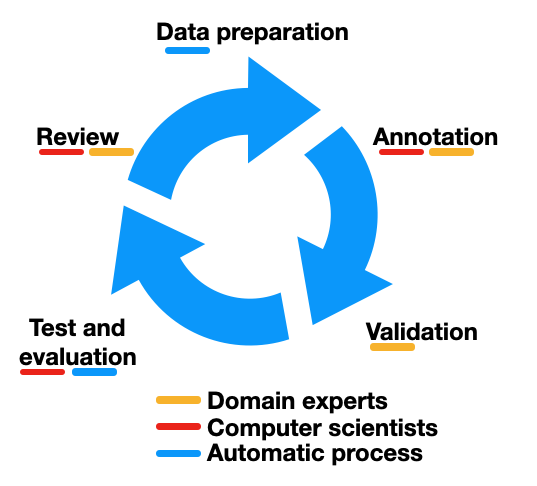
\includegraphics[width=0.5\linewidth]{figures/supermat/Fig2.png}
  \caption{Annotation workflow. Different colours illustrate the involvement of each group at each step of the workflow.}
  \label{fig:schema-comparison-modified-workflow}
\end{figure}

The first step of the annotation process involves preparing the machine-based annotated data from the source PDF documents. 
The PDF files are converted to an XML-based format, and annotation is automatically applied. 
This is followed by four more steps: 

\begin{itemize}
\item Annotation: The human annotator can select a document and manually add, remove, or modify each entity based on rules defined in the guidelines. Once the annotation is complete, the document is marked "ready" for the validation. 

\item Validation/Curation by domain experts: Annotations from different users are validated and merged into a final document (Figure~\ref{fig:inception-curation-interface}). 
The domain expert ("curator"), can compare the different annotated versions, and select the best combination of annotations, or add new ones. 
This step ensures that the annotations are cross-checked and that the document is validated by domain experts.

\item Automatic consistency checks and statistical analysis: This step aims to discover obvious mistakes such as mislabelling or incorrect linking. 
A sequence labelling model is trained and evaluated using 10-fold cross-validation. The evaluation provides precision, recall, and f-score metrics for all the labels.
The resulting model is used for producing machine-based annotated data in the following iteration.

\item Review: Retrospective analysis of the past iteration, where unclear cases are discussed and documented in the annotation guidelines. 

\end{itemize}

\subsection{Data transformation}
\label{subsec:transformation-of-data}
There are two processes of data transformation (Figure~\ref{fig:data-transformation}): (a) from the source document (PDF) to the dataset format representation (XML-based), and (b) from the dataset format representation to the annotation tool exchange formats (\url{https://inception-project.github.io/releases/0.16.1/docs/user-guide.html\#sect_formats}) and vice-versa. 

\begin{figure}[htb]
    \centering
    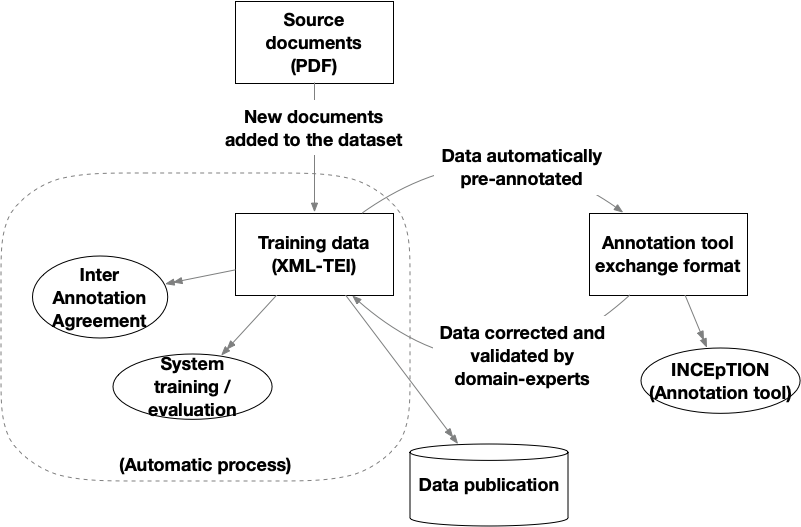
\includegraphics[width=\linewidth]{figures/supermat/Fig3.png}
    \caption{Summary of the data transformation flows.}
    \label{fig:data-transformation}
\end{figure}

\begin{itemize}
    \item PDF to XML-based: This step converts the PDF source document to the dataset format representation in XML following the Text Encoding Initiative (TEI, \url{https://tei-c.org/}) format guidelines. 
    Such transformation is performed by leveraging the functionalities provided by GROBID (\url{https://github.com/kermitt2/grobid}).
    
    We developed a customised process for collecting a subset of information from the source PDF document.
    The process extracts the title, keywords, and abstract from the header; and paragraphs, sections. and figure and table captions from the body.
    All the callouts to references, tables, and figures are ignored.
    The resulting structured document is then encoded in XML as will be described below. 
    \item XML to the annotation tool exchange formats: We transform our XML-formatted data into an INCEpTIONS compatible import format, such as the Webanno TSV 3.2 (\url{https://inception-project.github.io/releases/0.17.0/docs/user-guide.html\#sect_formats_webannotsv3}), and vice-versa using a set of Python scripts. 
    The Webanno TSV 3.2 format is an extension of the CONLL (\url{https://www.signll.org/conll/}) format, with additions of the header and column representation.
\end{itemize}

\section{Data Record}
\label{sec:data-record}
The dataset is composed of 142 PDF documents, of which 92\% (130) are OA (Figure~\ref{fig:arxiv-rate}).
To comply with copyright restrictions, a few articles from our dataset are not publicly available in our repository. 
The top three publishers represented in the corpus are the American Physical Society (APS), Elsevier, and IOP Publishing (Figure~\ref{fig:distribution-by-publisher}).
Figure~\ref{fig:distribution-by-year} illustrates the distribution by publication date.
We summarise SuperMat's content in Table~\ref{table:summary-content}, with the statistics of documents, entities, and links given separately. In particular, this dataset contains 16052 (7166 unique) entities spread over six labels and 1398 links. 

\begin{figure}[ht]
\centering
\subfloat[Papers distribution by Licence: Open Access vs copyrighted.]{\resizebox*{4cm}{!}{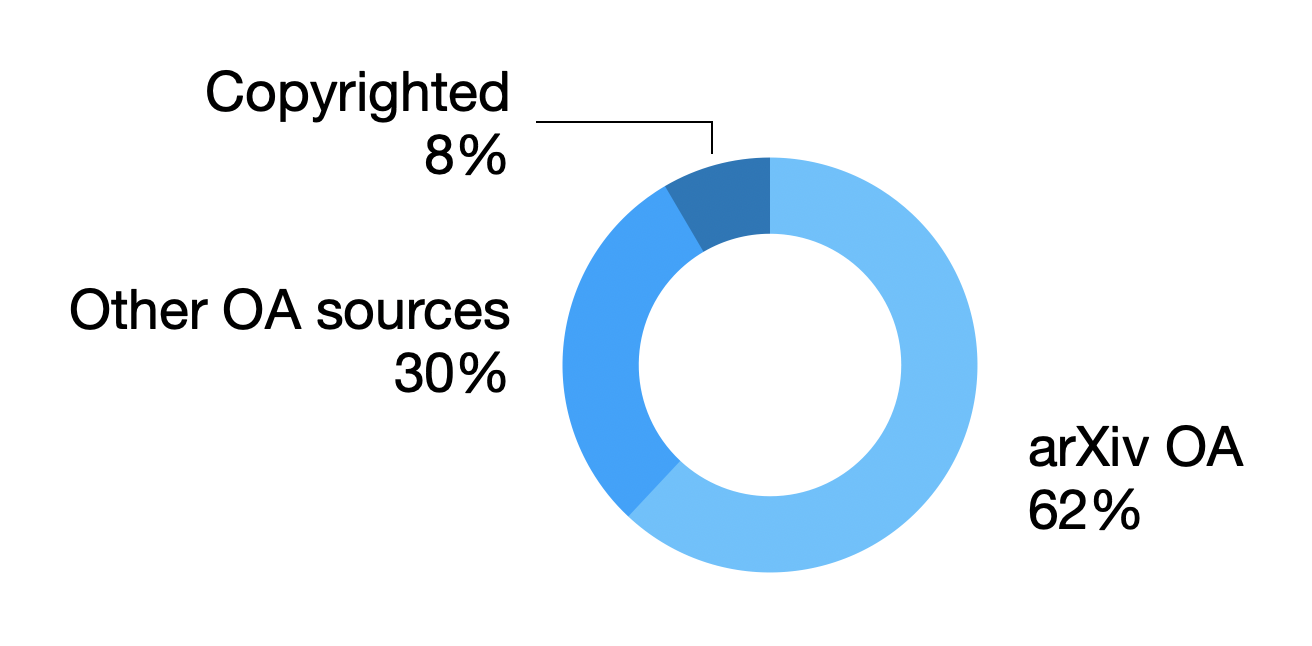
\includegraphics{figures/supermat/Fig4.png}}\label{fig:arxiv-rate}}
\hspace{5pt} 
\subfloat[Distribution by publisher.]{\resizebox*{4cm}{!}{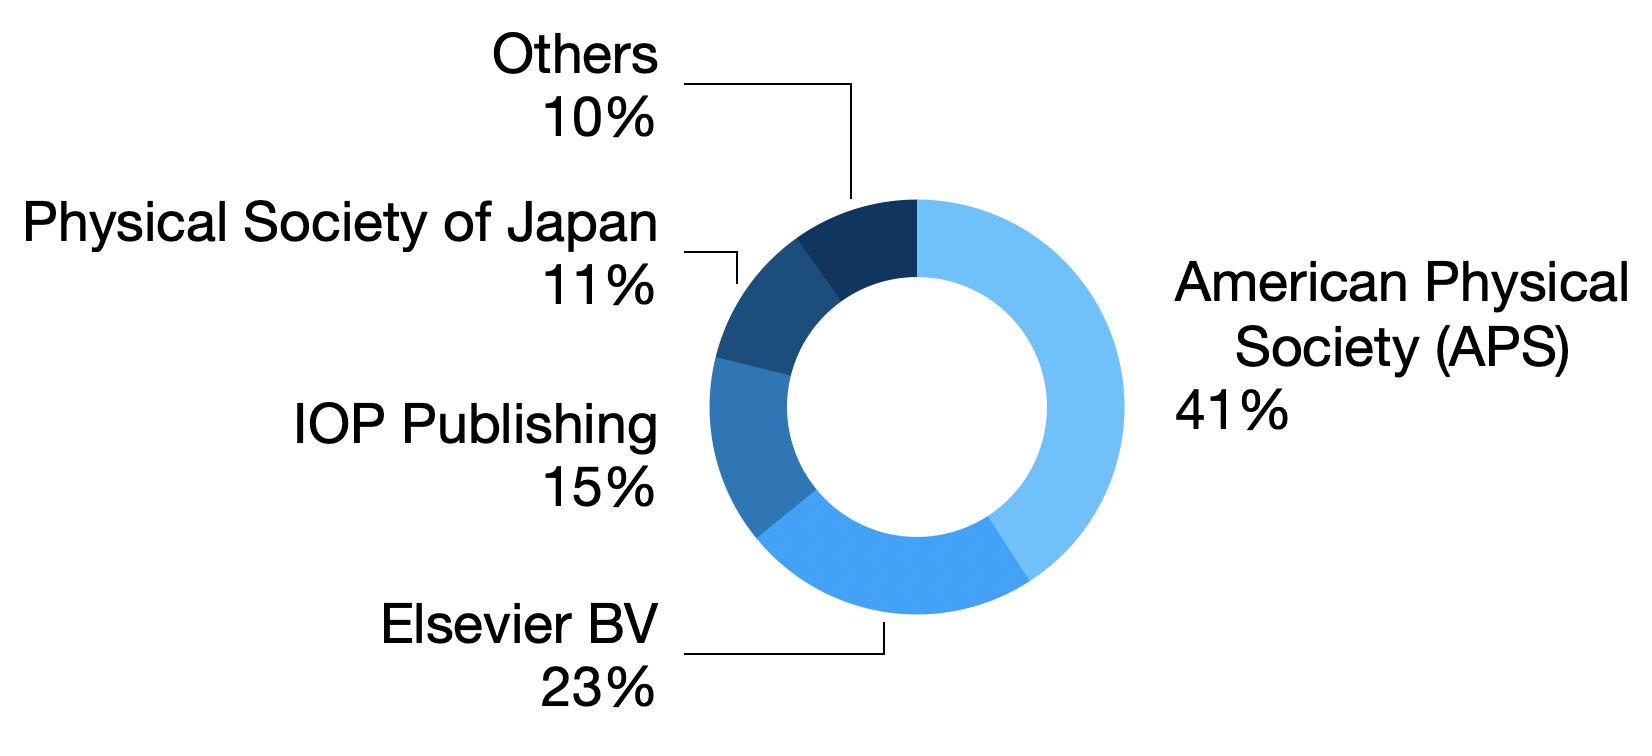
\includegraphics{figures/supermat/Fig5.png}}\label{fig:distribution-by-publisher}} 
\hspace{5pt} 
\subfloat[Distribution by year of publication.]{\resizebox*{4cm}{!}{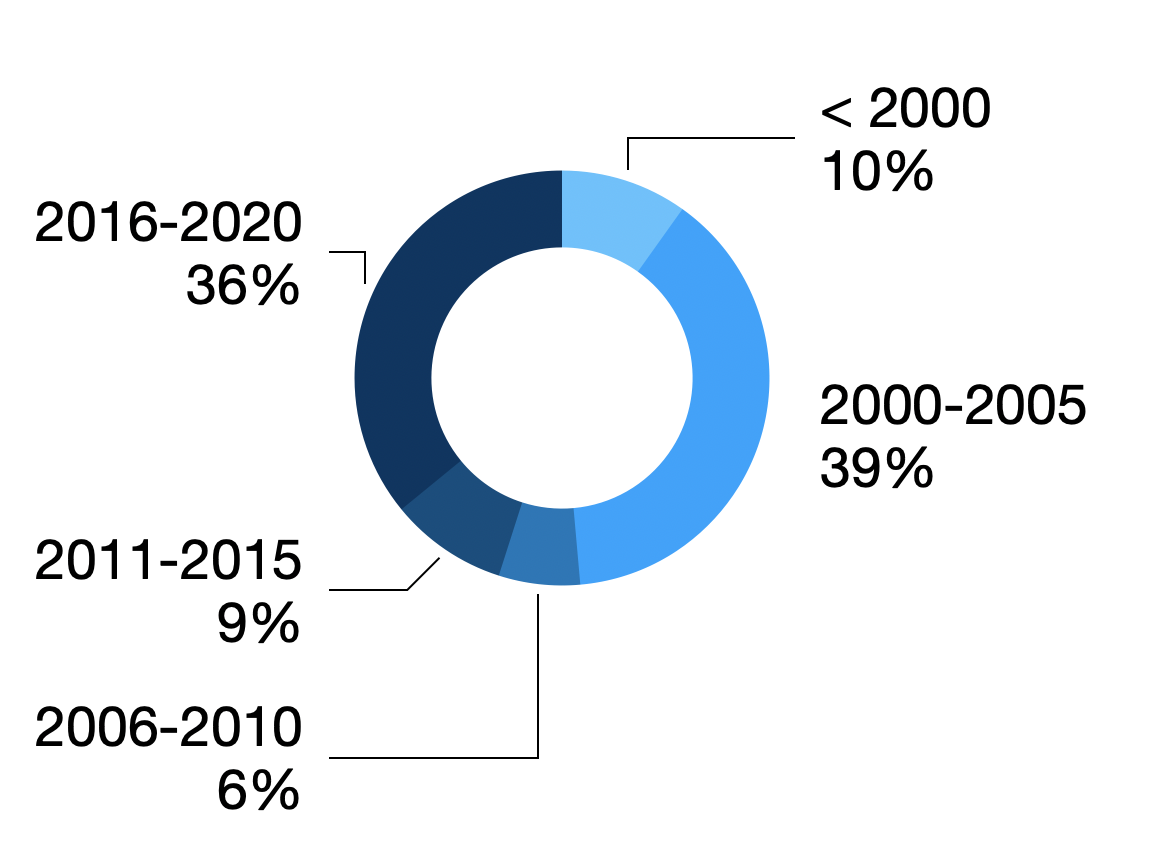
\includegraphics{figures/supermat/Fig6.png}}\label{fig:distribution-by-year}} 
\caption{Distribution of paper in the dataset by (a) license, (b) publisher, and (c) year of publication.} 
\label{fig:dataset-distributions}
\end{figure}

Each document is encoded according to the XML TEI guidelines, which is a rich format for document representation. 
We have carried out no specific customisation, in order to remain fully compliant with the general TEI schema.
A TEI document has two main parts: the header (within the \texttt{<teiHeader>} tags) containing all the document metadata, and the body (within the section delimited by the \texttt{<text>} tag). 
The transformed data has the following structure: 

\begin{verbatim}
<TEI xml:lang="en" xmlns="http://www.tei-c.org/ns/1.0">
    <teiHeader>
        <fileDesc>
            <titleStmt>
                <title>[...]</title>
            </titleStmt>
            <publicationStmt>
                <publisher>[...]</publisher>
            </publicationStmt>
        </fileDesc>
        <encodingDesc/>
            <abstract>
                <p>[...]</p>
                <ab type="keywords">[...]</ab>
            </abstract>
        <profileDesc>
        </profileDesc>
    </teiHeader>
    <text>
        <body>
            <p>[...]</p>
            <ab type="tableCaption"> [...] </ab>
            <p> [...] </p>
            <ab type="figureCaption"> [...] </ab> 
        </body>
    </text>
</TEI>
\end{verbatim}

We transformed the source documents into these TEI-compliant structures using a simplified representation for specific content types.
The general objective is to flatten the content into a generic structure where priority is given to the annotations.
For instance, the keywords section, which groups together the key terms defined by the author(s) of the paper, is encoded using the generic tag \texttt{<ab type="keywords">} as free text, instead of the dedicated \texttt{<keywords>} element that would typically be part of the header. 
For both the abstract and the article body, the text is segmented in paragraphs (by means of the \texttt{<p>} element). 
The text is annotated with the generic \texttt{<rs>} (referencing string) element adorned with three attributes: \texttt{@type} (the entity type), \texttt{@corresp} (to provide a link to another annotation such as from \textit{material} to \textit{T\textsubscript{c}}), and \texttt{@xml:id} (to uniquely identify the annotation for referencing or linking purposes).

Because only the captions of tables and figures are retained from the original source, a simplified encoding was defined by means of the \texttt{<ab>} element characterised by a \texttt{@type} attribute; that is, \texttt{<ab type="figureCaption">} for figure captions and \texttt{<ab type="tableCaption">} for table captions. 
Here is an example: 

\begin{verbatim}
<p>
    The electron-doped high-<rs type="tc">transition-
    temperature</rs> (<rs type="tc">Tc</rs>) <rs 
    type="class">iron-based pnictide</rs> 
    superconductor <rs type="material" 
    xml:id="m6">LaFeAsO1-xHx</rs> has a unique 
    phase diagram: Superconducting (SC) double domes are 
    sandwiched by antiferromagnetic phases at ambient 
    pressure and they turn into a single dome with 
    a maximum <rs type="tc">Tc</rs> that 
    <rs type="tcValue" xml:id="m7" 
    corresp="#m6,#9">exceeds 45K</rs> 
    at a pressure of <rs type="pressure" 
    corresp="#m7">3.0 GPa</rs>. 
    [...]
</p>
\end{verbatim}

In the above snippet, the entities \textit{"3.0 GPa"}, \textit{"exceed 45K"} and \textit{"LaFeAsO1-xHx"} are linked together via the pairs \texttt{@corresp, @xml:id}. 
This schema supports multiple annotations to any part of the document. 
For example, the entity \textit{exceed 45K} has a second link with the corresponding identifier (\textit{"\#9"}) to an annotation outside this paragraph.


\section{Applications}
\label{sec:applications}
SuperMat is constructed as a resource for TDM applications in superconducting materials. It can be used as data source in several complementary tasks: 
(1) creation of an automatic information extraction system for dataset creation,
(2) articles classification, 
(3) named entity extraction (for example, automatic dictionary construction), 
(4) clustering and document synthesis,
(5) training of machine learning (ML) algorithms,
(6) evaluation of rule-based or ML-based algorithms, and 
(7) development of downstream processes, such as material name parser, or quantity normalisation.

\subsection{Practical applications}
Such a dataset may benefit several types of possible applications: 

\begin{itemize}
    \item Evaluation tasks: This corpus can be used for evaluation tasks on automatic extraction. In particular, we can envision two popular tasks in superconducting materials science, namely: (a) NER and (b) EL methods. EL techniques have been mainly designed and studied using text from Wikipedia and newswires services which represent most of the available data. 
    To the best of our knowledge, however, there is no application within materials science.
    \item Automatic information extraction for superconducting materials: This dataset can be used as training data for such a purpose. 
    Automatic information extraction using ML and text mining techniques can accelerate the construction of databases for superconducting materials.
    \item Document retrieval: Information retrieval is a key application helping researchers overcome information overload.
    One way is through query expansion to cover multiple expressions of the same term. 
    By collecting and clustering all expressions under the same concept, it would be possible to retrieve documents when, for example, the resistivity measurement is described by a phrase other than "resistivity". 
    Furthermore, the assigned labels can be used to boost documents where a certain term belongs on a specific label. 
    For example, \textit{cobalt oxide} can appear as either \texttt{<material>} or \texttt{<class>} depending on the context, while a user would like to obtain documents where \textit{cobalt oxide} appears as \texttt{<material>}.
    \item Weighted-clustering: Scientific document clustering has recently gained growing attention because of its potential capacity for finding additional relevant documents of interest.
    For example, clustering can help locating similar experimental settings in a large collection of documents. However, clustering documents based on their general content might not be optimal for finding such detailed similarities.
    Annotation can be leveraged to tilt the clustering algorithm toward entity similarity, which may provide a more focused clustering towards a specific type of information.
\end{itemize}

\label{sec:technical-validation}
\section{Technical Validation} 
The following measures were employed to ensure the creation of a high-quality dataset: 
\begin{itemize}
    \item Each document was revised and validated by domain experts, 
    \item The workflow begins by assigning machine-based annotated data. This has demonstrated to improve the annotation task over several aspects, namely: time consumption, error rate, and annotation agreement~\cite{Fort2010InfluenceOP,Nvol2011SemiautomaticSA,Lingren2014EvaluatingTI}.
    \item On-the-fly automatic annotation recommendations, which provide fresh suggestions based on online decisions made by the annotators.
    \item The annotators have rapid access to changes in the annotation guidelines.
    \item The discussions were documented and linked in the guidelines. 
    \item Reviews are discussed and approved collaboratively between domain experts and other annotators.
\end{itemize}

\begin{table}[ht]
    \caption{Average IAA between the annotated and validated documents}
    \begin{tabular}{ cc } 
    \toprule
        \textbf{Label} & \textbf{Average}\\
    \midrule
        \texttt{<material>}     &   0.956   \\
        \texttt{<me\_method>}   &	0.887   \\
        \texttt{<pressure>}     &	0.723   \\
        \texttt{<class>}        &	0.925   \\
        \texttt{<tcValue>}      &	0.863   \\
        \texttt{<tc>}           &	0.831   \\
    \midrule
        \textbf{Micro average}        &	0.911	\\
    \bottomrule
    \end{tabular}
    
    \label{table:average-iaa}
\end{table}

These guidelines are a vital piece of this work since they contain knowledge accumulated from these activities.
However, measuring the completeness of the guidelines is challenging. 
Assuming that the documents validated by domain experts represent the ground truth, we conducted IAA analysis between different annotators against the ground truth, using the Krippendorf's Alpha metric~\cite{Krippendorff2004ReliabilityIC}.
Table~\ref{table:average-iaa} shows the average IAA which is satisfying with a value of approximately 0.9. 
The highest score is obtained in the \texttt{<material>} entities, while the lowest one is obtained in \texttt{<pressure>}, which appears less frequently in the papers. 
The disagreement in \texttt{<tcValue>} can appear to be too low as compared with other labels such as \texttt{<class>}, which is, at first look, more ambiguous. 
We analysed the different cases and identified three reasons why this happens. 
First, \texttt{<tcValue>} may depend heavily on the context that requires more human attention, and it is therefore more prone to errors. 
Second, our suggestions system is challenged in its ability to disambiguate critical temperatures from other temperature data, leading to incorrect or invalid suggestions. 
Finally, the presence of mathematical symbols (e.g. "\texttt{\~}", "\texttt{<}", and "\texttt{>}") or other modifiers ("\texttt{up to}", "\texttt{exceeds}", etc.) before the \texttt{<tcValue>} could generate small disagreements that accumulate in the average score. 

\begin{table}[ht]
     \caption{Calculated IAA for annotations produced by domain experts, non-domain experts, and novices compared to the validated version. Annotations from domain experts are cross validated. }
    \begin{tabular}{ ccccc } 
    \toprule
        \textbf{Label} & \textbf{Domain experts} & \textbf{Non-domain experts} & \textbf{Novices}\\
    \midrule
        \texttt{<material>}     &   0.969   & 0.950    &   0.924   \\
        \texttt{<me\_method>}   &   0.890   & 0.862    &   0.901   \\
        \texttt{<pressure>}     &   0.836   & 0.741    &   0.746   \\
        \texttt{<class>}        &   0.990   & 0.836	   &   0.899   \\
        \texttt{<tcValue>}      &   0.895   & 0.734	   &   0.841   \\
        \texttt{<tc>}           &   0.874   & 0.776	   &   0.830   \\
    \midrule
        \textbf{All labels}        &	0.940   &   0.882	&      0.896   \\
    \midrule
        \textbf{\# paragraphs}  &   1066   &  1648	    &   325     \\
    \bottomrule
    \end{tabular}
   
    \label{table:comparison-iaa-nde-de}
\end{table}

To more precisely isolate the impact of the guidelines, we grouped the IAA results by level of domain experience. 
Table~\ref{table:comparison-iaa-nde-de} displays the IAA between the validated data and the data corrected by (a) domain experts (researchers who conduct superconducting development experiments), (b) non-domain-experts (researchers with no experience with superconducting materials), and (c) novices (students in materials science with limited domain experience). 
Obviously, the domain experts have the highest agreement and the IAA value (around 0.95) is 0.06 higher on average than that of non-domain experts. 
Thus, superconducting materials is a complex domain that requires knowledge in materials science to produce high-quality data, while crowdsourcing initiatives such as the Amazon Mechanical Turk might not work well. 

Furthermore, we measured the reliability of the guidelines by observing how quickly novices could reach a satisfying agreement with the validation of the domain experts, without any previous training on the guidelines.
From Table~\ref{table:comparison-iaa-nde-de}, the  novices can attain high IAA results by only using the guidelines and our annotation support tools. 
The average difference in agreement with domain experts (around 0.05) indicates that the guidelines are precise and complete, and that the annotations tools offer sufficient support. 

\section{Data Availability}
\label{sec:code-availability}
The references of the original papers and their bibliographical information, the annotation guidelines sources, and the developed code are available at the GitHub repository \url{https://github.com/lfoppiano/SuperMat}. The guidelines are freely accessible at \url{https://supermat.readthedocs.io}.
The data transformation scripts were written in Python and can be run from the command line. 
They require BeautifulSoup  (\url{https://www.crummy.com/software/BeautifulSoup/}), an open-source library for parsing XML and HTML formats. 
The data analysis scripts were developed as Jupyter notebooks (\url{https://jupyter.org/}) which can easily output results and graphs in the browser. 
The open source annotation tool is INCEpTION (\url{https://inception-project.github.io/}). 
The content was acquired using biblio-glutton (\url{https://www.github.com/kermitt2/biblio-glutton}) and Grobid (\url{https://www.github.com/kermitt2/grobid}).
We computed the IAA using the Java library DkPro statistics (\url{https://dkpro.github.io/dkpro-statistics/})~\cite{Meyer2014DKProAA}.

% inception-curation-new.png
\begin{figure}[htb]
    \centering
    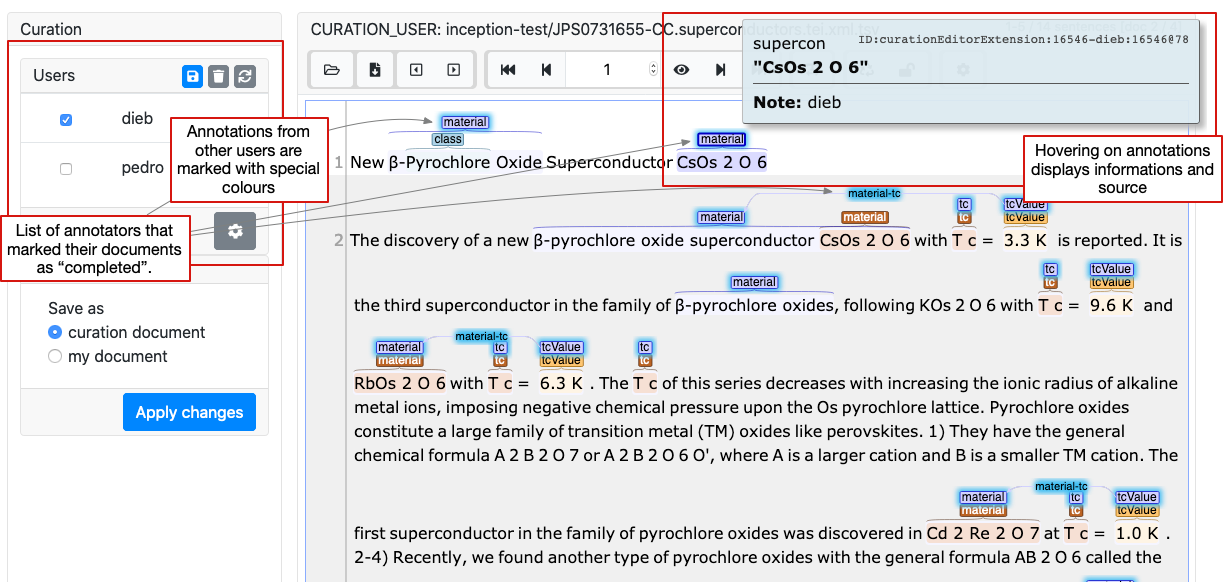
\includegraphics[width=\linewidth]{figures/supermat/Fig7.png}
    \caption{INCEpTION curation interface. Excerpt from © 2004 The Physical Society of Japan (J. Phys. Soc. Jpn. 73, 1655-1656)}
    \label{fig:inception-curation-interface}
\end{figure}















\chapter{Automatic identification and normalization of physical quantities from scientific publications}
\label{cha:measurements}

% \section{Introduction}
% \section{Main contributions}
% \section{Experiments}
% \section{Conclusion}


\section{System description}
\label{sec:system}
Grobid-quantities is a Java web application, based on Grobid (GeneRation Of BIbliographic Data)~\cite{GROBID} \cite{lopez2009grobid}, a machine learning framework for parsing and structuring raw documents such as PDF or plain text. 
Grobid-quantities is designed to process large quantity of data, via web, through a REST (Representation State Transfer) API or locally, via the file-system (batch mode). 
Output information are standardised as stand-off annotations, and they can be stored in databases or indexed in search engines. Each annotation can be visualised on top of PDFs using the GROBID build-in positional coordinates.

\subsection{Data model}
\label{subsub:data-model}
\begin{figure}[ht]
  \centering
  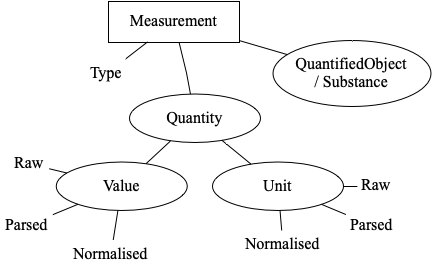
\includegraphics[width=\linewidth]{figures/quantities/schema-2.png}
  \caption{Schema of the data model.}
  \label{fig:data-model-schema-2}
\end{figure}

The data model (Figure \ref{fig:data-model-schema-2}) lay its foundation on the concept of \textit{Measurement}, which links an object or a substance with one or more \textit{quantities}. We defined four \textit{Measurements} types: (a) atomic, in case of a single measurement (e.g., 10 grams). (b) interval (\textit{from 3 to 5 km}) and (c) range ($100 \pm 4$ mm) for continuous values, and, (d) a list of discrete values. A \textit{Quantity} links the quantitative value and the unit. 
Since data extracted from PDFs unavoidably present irregular tokens from wrong UTF-8 encoding or missing fonts, we designed this model to allow partial results. The \textit{Value} and \textit{Unit} entities allow three different representations (Figure \ref{fig:data-model-schema-2}): \textit{Raw} as appear in input, \textit{Parsed} unifies the value into the numerical expression, and the unit with its properties (system, type). Finally, \textit{Normalised} contains the transformed unit and values to the SI system. \textit{Value} object supports four types of representations: numeric (2, 1000), alphabetic (two, thousand), scientific notation ($3\cdot10\textsuperscript{5}$), and time, which is also an expression of measurement. Units objects are organised following the SI, which allows representing units as products of simpler compounds (e.g. m/s to $m \cdot s\textsuperscript{-1}$) further decomposed as triples (prefix, base and power).

\subsection{Architecture}
The system takes in input text or PDF (the content is extracted in a structured way using the Grobid framework) and performs three steps: (a) tokenisation, (b) measurement extraction and parsing and (c) quantity normalisation. The details of each step are summarised as follows. 

\subsubsection{Tokenisation}
This process splits input data into tokens. Grobid-quantities uses a two-phase tokenisation: (1) first it splits by punctuation marks, then (2) each resulting token is re-tokenised to separate adjacent digits and alphanumeric characters. Given the example \texttt{25m\^{}2}, first returns a list \texttt{[25m, \^{}, 2]} and then recursively divides \texttt{25m} as \texttt{[25, m]}  resulting in \texttt{[25, m, \^{}, 2]}.

\subsubsection{Extraction}
% Quantity model 
The tokens are passed through three ML models, in cascade: first the \textit{Quantities} CRF model determines appropriate unit and value tags. Results are further processed by the respective \textit{Units} and \textit{Values} CRF models as illustrated in Figure \ref{fig:schema-cascade}.  

\begin{figure}[ht]
  \centering
  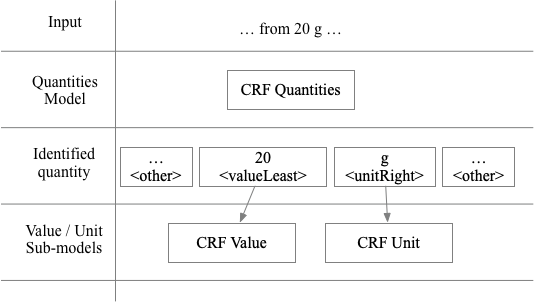
\includegraphics[width=\linewidth]{figures/quantities/schema-cascade}
  \caption{The cascade approach in applied CRF models. The Quantities model recognises value and units which are passed, respectively, to Values and Units CRF sub-models for further extraction.}
  \label{fig:schema-cascade}
\end{figure}

Table \ref{tab:quantities-model-labels} describes the labels predicted by the \textit{Quantities} CRF model. Notice that, to reconstruct complex structured objects from the flat sequence generated by the engine, additional labels are necessary (such as <unitLeft>, <unitRight>, for units).

\begin{table}[ht]
\centering
  \caption{Labels description for the Quantities CRF model. In bold are highlighted specific examples.}
  \label{tab:quantities-model-labels}
  \begin{tabular}{lll}
    \toprule
    Label & Description & Example\\
    \midrule
    valueAtomic & value of an atomic quantity & \textbf{2} m \\
    valueLeast & least value in an interval & from \textbf{2} m \\
    valueMost & max value in an interval & up to \textbf{7} m \\
    valueBase & base value in a range & $\textbf{20}\pm7$ m \\
    valueRange & range value in a range & $20 \pm \textbf{7}$ m \\
    valueList & list of quantities & \textbf{2}, \textbf{3} and \textbf{10} m \\
    unitLeft & left-attached unit & \textbf{pH} 2 \\
    unitRight & right-attached unit & 2 \textbf{m} \\
    other & everything else & - \\
  \bottomrule
\end{tabular}
\end{table}

% Gazetteers
Previous work presented extensive use of databases or ontologies. In our solution, we used a similar approach. We created a list of units (in English, French and German) with their characteristics: system (SI base, SI derived, imperial, ...) and type (volume, length, ...), and their representations: notations (m\textsuperscript{3}, \texttt{m\^{}3}), lemmas (cubic meter, cubic metre) and inflections (cubic meters, cubic metres). We made this list available through the \textit{Unit Lexicon}, which offers unit lookups by properties (such as notation, lemma, inflexion). A second gazetteer was created to allow the transformation of alphabetic values in numeric ones (for example, twenty-one to 21).

Features in the \textit{Quantities} CRF model are generated from preceding and following tokens, presence of capital, digits. Orthogonal features are obtained through the \textit{Unit Lexicon}, like a \textit{Boolean} indicating whether a token is a known unit or not. Typographical information (such as format, fonts, subscript and superscript) are ignored. 

% Unit model 
The \textit{Units} CRF model works at character level and uses the \textit{Unit Lexicon} to highlight known units or prefixes. The input tokens are parsed and transformed to a product of triples (prefix, base, power) as shown in Table \ref{tab:units-model-labels}. For example \texttt{Kg/mm\textsuperscript{2}}, corresponds to \texttt{$Kg\cdot mm\textsuperscript{-2}$} and becomes \texttt{[(K, g, 1), (m, m, -2)]} as product of triples. 

\begin{table}[ht]
\centering
  \caption{Labels description for the Units CRF model. In bold are highlighted specific examples. }
  \label{tab:units-model-labels}
  \begin{tabular}{lll}
    \toprule
    Label & Description & Example\\
    \midrule
    prefix & prefix of the unit  & \textbf{k}m\textsuperscript{2} \\
    base & unit base & k\textbf{m}\textsuperscript{2}\\
    pow & unit power & km\textsuperscript{\textbf{2}}\\
    <other> & everything else & - \\
  \bottomrule
\end{tabular}
\end{table}

We then use the structured triples to fetch the corresponding information (system, type) from the \textit{Unit Lexicon} and attach them to the resulting object. 
This implementation processes the unit characters using right-to-left order. 
%Priority modifiers, such as parenthesis, are ignored because more complex to manage and not frequent. 
Priority modifiers, such as parenthesis, are ignored. They are generally not frequent in units expressions, and require a more complex logic.

%Let's suppose the raw text contains "10 m 3". The Quantity model identifies 10 as atomic value and "m 3" as the unit. The Unit model identifies "m" as the base and "3" as power: [(,m,3)]. This product is then reformatted as "m\^3" and looked up in the gazetteer. Since "m\^3" exists, system=SI, inflection='Cubic meters' and type=volume are attached to the unit object. 
% Value model 
In parallel, the CRF \textit{Values} model unifies the format of identified values into numerical formats. It supports four types: numeric, alphabetic, scientific notation, and time expression (see Table \ref{tab:values-model-labels}). Different techniques are applied for each type: alphabetic expressions are looked up in the word-to-number gazetteer, scientific notations are parsed and calculated mathematically. Time expressions are further segmented using the Grobid built-in Date CRF model.

\begin{table}[ht]
\centering
  \caption{Labels description for the Values CRF model. In bold are highlighted specific examples.}
  \label{tab:values-model-labels}
  \begin{tabular}{lll}
    \toprule
    Label & Description & Example\\
    \midrule
    \texttt{number} & numeric value / coefficient & $\textbf{2.5}\cdot10\textsuperscript{\textbf{5}}$ \\
    \texttt{alpha} & alphabetic value & \textbf{twenty} \\
    \texttt{time} & time expression  & in \textbf{1970-01-02}\\
    \texttt{base} & base in scientific notation & $2.5\cdot\textbf{10}\textsuperscript{5}$\\
    \texttt{pow} & exponent in scientific notation & $2.5\cdot10\textsuperscript{\textbf{5}}$ \\
    \texttt{other} & everything else & - \\
  \bottomrule
\end{tabular}
\end{table}

\subsubsection{Normalisation}

The measurements extracted are transformed to the base SI unit (grams to kg, Celsius to Kelvin, etc.). We used an external Java library called Units of Measurement~\cite{units_of_measurement}, which provides a set of standard interfaces and implementations for safely handling units and quantities. Manipulating measurements with transformations often lead to common mistakes due to wrong rounding and approximations. 
At the time this paper is being written, the final revised version of this library has been accepted under the Java Standardisation Process JSR-385.

\section{Evaluation and results}
\label{sec:results}

We trained and evaluated our system's models using a dataset based on 32 scientific publications (English, Open Access (OA)) and three patents (with translation in English, French and German) randomly selected from different domains such as medicine, robotics, astronomy, and physiology. The training data was generated automatically and then corrected and cross-checked by three annotators. We used 10-fold cross-validation to evaluate each CRF model, independently, and produce precision, recall and f1 scores, as summarised in Table \ref{tab:quantities-evaluation}. 

\begin{table}[ht]
    \centering
   \caption{Summary of the evaluation scores (precision, recall, F1-score) and label contribution (support) for \textit{Quantities}, \textit{Units} and \textit{Values} CRF models, respectively. }
   \label{tab:quantities-evaluation}
   \begin{tabular}{c|cccc}
        \toprule
        Label & Precision & Recall & F1 & Support\\
        \toprule
        \multicolumn{5}{c}{\textbf{Quantities CRF model}}\\
        \midrule
        \texttt{unitLeft}          & 96.76 & 94.71 & 95.71 & 2805  \\
        \texttt{unitRight}         & 93.06 & 72.1  & 80.02 & 120   \\
        \texttt{valueAtomic}       & 85    & 84.77 & 84.84 & 3599  \\
        \texttt{valueBase}         & 78.82 & 76.52 & 77.53 & 94    \\
        \texttt{valueLeast}        & 85.05 & 77.39 & 80.94 & 862   \\
        \texttt{valueList}         & 72.09 & 54.87 & 61.33 & 494   \\
        \texttt{valueMost}         & 84.09 & 73.03 & 78.07 & 878   \\
        \texttt{valueRange}        & 84.56 & 81.5  & 82.68 & 93    \\
        all (macro avg.)    & 84.93 & 76.86 & \textbf{80.14}\\
        \midrule
        \multicolumn{5}{c}{\textbf{Unit CRF model}}\\
        \midrule
        \texttt{base}              & 99.02 & 99.22 & 99.12 & 3075      \\
        \texttt{pow}               & 98.04 & 98.9  & 98.46 & 322       \\
        \texttt{prefix}            & 99.19 & 98.8  & 98.99 & 821       \\
        all (macro avg.)    & 98.75 & 98.97 & \textbf{98.86}    \\
        \midrule
        \multicolumn{5}{c}{\textbf{Values CRF model}}\\
        \midrule
        \texttt{alpha}             & 96.64  & 98.65 & 97.62  & 826      \\
        \texttt{base}              & 83.06  & 69.23 & 72.77  & 58       \\
        \texttt{number}            & 98.01  & 99.02 & 98.52  & 3858     \\
        \texttt{pow}               & 76.45  & 74.67 & 74.58  & 56       \\
        \texttt{time}              & 72.54  & 87.83 & 79.34  & 322      \\
        all (macro avg.)    & 85.34  & 85.88 & \textbf{84.57} & -\\
        \bottomrule
   \end{tabular}
\end{table}

% Scores + discussion Quantities CRF model 
The Quantities CRF model reported an f1 macro average of 80.14\% with precision and recall of 84.93\% and 76.86\%, respectively. The paragraph accuracy was 68.97\%, indicating that more than half of the evaluated paragraphs were correctly labelled. These scores are promising, considering the complexity of the task and the rather small size of the training corpus. In particular, \texttt{<list>} and \texttt{<unitRight>} require more example. 

% Scores + discussion Unit CRF model 
The Units CRF model f1 macro average was 98.86\%, with precision and recall reaching 98.75\% and 98.97\%, respectively. Compared with our other models, performances were extremely high (more than 10\% for f1 score). 
Such difference can be attributed to the data distribution and the lower variability of unit expressions. We analysed the training data, and we noticed that the distribution is biased toward simple units (composed by a single triple). Intuitively, this makes sense, because simple units are statistically more frequent; on the other hand, it highlights the necessity of having more complex examples in our dataset. 
Secondly, unit expressions appear, by nature, with lower variability, leading to the generation of more duplicates than in other models' training datasets. For example, the expressions 1\% and 2\% have two different values (1, 2) and the same unit (\%), which would appear twice. 
Since we cannot alter the statistical distribution of the dataset, we would obtain better and more precise measurements of the model generalisation capabilities by using a separate and independent evaluation corpus. 

% Scores + discussion Values CRF model 
The Value CRF model scored average macro f1 at 85.64\% with precision and recall at 81.82\% and 93.29\%, respectively.
We noticed that both \textit{<base>}, \textit{<pow>} and \textit{<time>} have lower f1-score. While \textit{<base>} and \textit{<pow>} require more training data, \textit{<time>} expressions may overlap with \textit{<number>} suggesting more contextual information should be introduced. 


\section{Applications}
\label{sec:use_cases}
Recently, the normalised data extraction is strongly required in materials research. The inverse problem in which high-performance materials are predicted from properties is expected to be solved with well-organised big data. At the National Institute for Materials Science (NIMS), a project to discover new superconducting materials from scientific literature is in progress. The system being developed relies on Grobid-quantities to extract and normalise superconducting properties, such as critical temperature (Tc) with units of mK and K and critical pressure expressed with units of Pa, MPa, and GPa \cite{foppiano2019proposal}. 

Grobid-quantities was showcased in a Text and Data Mining (TDM) platform (within the scope of the French national-wide ISTEX~\cite{dazy2014istex} project) where it provided measurement annotations used to prototype a quantities-based semantic search\footnote{The demo can be accessed at \url{https://traces1.inria.fr/istex_sample/}}. 

Finally, another use was made in a system for extracting semantic measurements and meaning in Earth Science, Marve~\cite{hundman2017measurement}.  

\chapter{Semi-automatic staging area for high-quality structured data extraction from scientific literature}
\label{cha:curation}
\chapter{Semi-automatic staging area for high-quality structured data extraction from scientific literature}

\section{Curation workflow}
\label{sec:curation-workflow}
The curation of the SuperCon\textsuperscript{2} Database acts as a workflow where user actions result in database records state transitions (Figure~\ref{fig:curation-workflow}). 
Allowed manual actions include a) \textit{mark as valid} (validation) when a record is considered correct or corrected by someone else. When a record is not valid, users can: b) \textit{mark as invalid} when considered ``potentially'' invalid (or the curator is not confident), c) perform \textit{manual correction} to update it according to the information from the original PDF document, and d) \textit{remove} the record when it was not supposed to be extracted.

Besides manual operations from users, this workflow supports also automatic actions: ``anomaly detection'' for pre-screening records (Section~\ref{subsec:anomaly-detection}) and the ``training data collector'' for accumulating training data for improving ML models (Section~\ref{subsec:feedback-loop-training-data}). 

% Once a structured database is collected, its data can be visualised and curated by domain experts. 
% The curation process can be delineated as a structured workflow, wherein each record undergoes a series of transitions between distinct states determined by the actions that are executed on the record (Figure~\ref{fig:curation-workflow}).

Although only the most recent version of a record can be viewed on this system, the correction history is recorded (Section~\ref{subsec:curation-and-processing-logs}). 


\begin{figure}[ht]
  \centering
  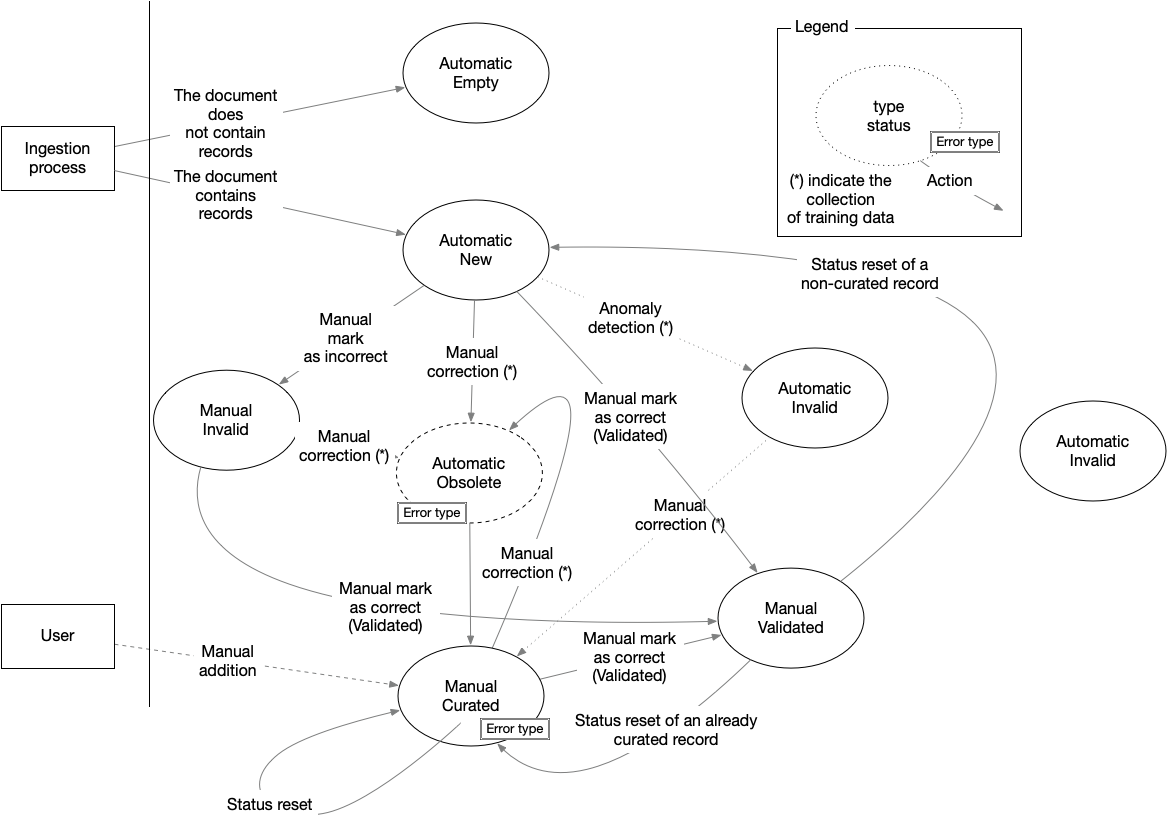
\includegraphics[width=1\textwidth]{figures/curation/record-correction} 
  \caption{Schema of the curation workflow. Each node has two properties: type and status (Section~\ref{subsec:curation-status}). Each edge indicates one action. The workflow starts on the left side of the figure. The new records begin with ``Automatic, New''. Changes of state are triggered by automatic (Section~\ref{subsec:anomaly-detection}) or manual operations (update, mark as valid, etc.. Section~\ref{subsec:manual_correction}) and results in changes of the properties in the node. Each combination of property values identifies each state. ``(*)'' indicates a transition for which the training data are collected (Section~\ref{subsec:feedback-loop-training-data})}
  \label{fig:curation-workflow}
\end{figure}

% When a record (\emph{original record}) is updated (\emph{updated record}) 
% Both records are persisted in every state of the workflow, only the latest being visible.
% Similarly, when a record is removed the data is kept but the record is hidden, while records marked as valid or invalid are kept visible. 

% The workflow establishes also that when a record is manually corrected, the raw data from which the record has been extracted, are collected as training data (Section~\ref{subsec:feedback-loop-training-data}).

\subsection{Workflow control}
\label{subsec:workflow-control}
The workflow state is determined by the ``curation status'' (Section~\ref{subsec:curation-status}), the user action, and the error type (Section~\ref{subsec:error-types}).

\subsubsection{Curation status} 
\label{subsec:curation-status}
The curation status (Figure~\ref{fig:curation-workflow}) is defined by \emph{type} of action, manual or automatic, and \emph{status}, which can assume the following values: 
\begin{itemize}
    \item \textbf{new}: default status when a new record is created.
    \item \textbf{curated}: the record has been amended manually.
    \item \textbf{validated}: the record was manually marked as valid.
    \item \textbf{invalid}: the record is wrong or inappropriate for the situation (e.g., T\textsubscript{m} or T\textsubscript{curie} extracted as superconducting critical temperature).
    \item \textbf{obsolete}: the record has been updated and the updated values are stored in a new record (internal status\footnote{``internal status'' indicates that their records should be hidden in the interface}).
    \item \textbf{removed}: the record has been removed by a curator (internal status).
\end{itemize} 
    

% For example, the value "automatic" is provided when the data is ingested (Section~\ref{sec:ingestion}) or when the "anomaly detection" detects incorrect values and performs operations such as marking the record "invalid". 
% The "type" can change from "automatic" to "manual" but never in the opposite direction, because automatic operations are never applied on validated or curated records.

\subsubsection{Error types}
\label{subsec:error-types}
We first introduced \emph{error type} in~\cite{foppiano2023automatic} and extended their scope in this work to consider data curation and anomaly detection. 

Users are required to select one \emph{Error Type} at every record update or removal. This information is stored in the ``original'' record and can be different at every record modification.
The error type values can be summarised as follows: 

\begin{itemize}
    \item \textbf{From table}: the entities Material $\rightarrow$ T\textsubscript{c} $\rightarrow$ Pressure are identified in a table. At the moment, table extraction is not performed
    \item \textbf{Extraction}: The material, temperature, and pressure are not extracted (no box) or extracted incorrectly. 
    \item \textbf{Linking}: The material is incorrectly linked to the T\textsubscript{c} given that the entities are correctly recognised.
    \item \textbf{T\textsubscript{c} classification}: The temperature is not correctly classified as ``superconductors critical temperature'' (e.g., Curie temperature, Magnetic temperature...).
    \item \textbf{Composition resolution}: The exact composition cannot be resolved (e.g., the stoichiometric values cannot be resolved).
    \item \textbf{Value resolution}: The extracted formula contains variables that cannot be resolved, even after having read the paper. This includes when data is from tables
    \item \textbf{Anomaly detection}: The data has been modified by anomaly detection, which facilitates their retrieval from the interface.
    \item \textbf{Curation amends}: The curator is updating the data which does not present issues due to the automatic system.
\end{itemize}

\subsection{Anomaly detection}
\label{subsec:anomaly-detection}
Anomaly detection is the process of identifying unusual events or patterns in data. 
In our context, this means identifying data that are greatly different from the expected values.
This post-process was introduced in a limited scope to draw attention to certain cases during the curation.

The anomaly detection uses a rule-based approach and marks any record that matches the following conditions
\begin{itemize}
    \item the extracted T\textsubscript{c} is greater than room temperature (273 K), negative, or contains invalid characters and cannot be parsed (e.g. ``41]'')
    \item the chemical formula cannot be processed by an ensemble composition parser that combines Pymatgen~\cite{Ong2013}, and text2chem~\cite{kononova2019text} 
    \item the extracted applied pressure cannot be parsed or falls outside the range 0 - 250 GPa.
\end{itemize}

Records identified as anomalies have \emph{status} ``invalid'' and \emph{error type} ``anomaly detection'' for easy identification.
Since this process may find false positives, its output requires validation from curators. 
For example, in certain contexts, T\textsubscript{c} values above room temperature or applied pressure up to 500 GPa may be valid in researchers' hypotheses, calculations, or simulated predictions. 

We ran the anomaly detection on the full SuperCon\textsuperscript{2} Database (40324 records~\cite{foppiano2023automatic}). 
The anomaly detection identified 1506 records with invalid T\textsubscript{c}, 5021 records with an incomplete chemical formula, 304 records with invalid applied pressure, and 1440 materials linked to multiple T\textsubscript{c} values. 
Further analysis and cross-references with contrasting information may be added in future. 

\subsection{Automatic training data collector}
\label{subsec:feedback-loop-training-data}
The curation process is a valuable endeavour demanding significant knowledge and human effort. 
To maximise the use of this time for collecting as much information as possible.
We integrated an automatic procedure in the curation process that, for every correction, accumulates the related data examples that can be used to improve the underlying ML models. 
% In Section~\ref{subsec:training-data-generation-evaluation} we evaluate its this approach helps improve the ML model with a small number of examples as compared with the training dataset. 

\subsubsection{Training data collection}
In the event of a correction (update, removal) in a database record, this process retrieves the corresponding raw data: the text passage, the recognised entities (spans), and the layout tokens information. 
This information is sufficient to be exported as training examples, which can be examined and corrected, and feedback to the ML model. 
% In detail, the process performs the following actions:
% \begin{itemize}
%     \item The updated record is prepared and stored.
%     \item The raw data originating the updated record is identified. First, the corresponding structured document is retrieved from the document collection using the document identifier (the hash). Then, the exact text passage in the structured document is located using a unique id assigned to each material in the database records.
%     \item If the raw data has already been collected, it is skipped. This is the case when multiple records belonging to the same text passage are corrected.
%     \item Otherwise, the raw information comprising the text string, the spans, and the layout tokens are collected and saved in a separate collection.
%     \item The data collected is then sufficient to generate workable instances in different output formats and the related feature files.
% \end{itemize}

\subsubsection{Training data management}
We designed a specific page of the interface (Section~\ref{sec:user-interface}) to manage the collected data (Figure~\ref{fig:training-data-view}) in which each row corresponds to a training example composed by the decorated text showing the identified entities, the document identifier, and the status. 
The users can examine the data, delete it, send it to the annotation tool to be corrected, and then export them.
We integrated our interface with Label-studio~\cite{Label_Studio} for the correction of the collected training examples. 
Label-studio is an open-source, python-based, and modern interface supporting many different TDM tasks (NER, topic modelling, image recognition, etc.). 

\begin{figure}[ht]
  \centering
  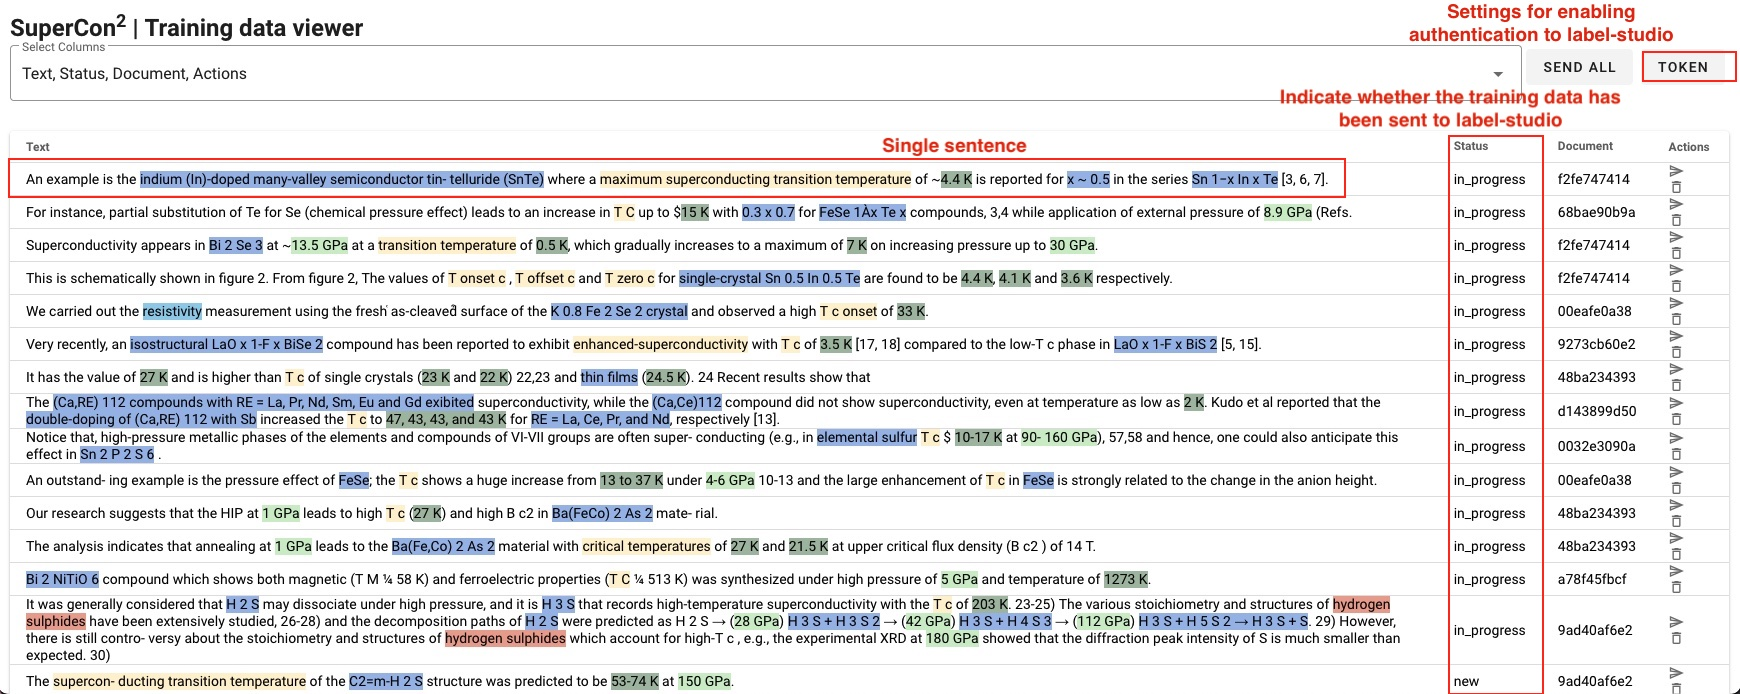
\includegraphics[width=1\textwidth]{figures/curation/training-data-viewer} 
  \caption{Screenshot of the training data management page in the SuperCon\textsuperscript{2} interface. Each row contains one potential training data example. Each example is composed of a sentence and its extracted entities (highlighted in colour) with potential annotation mistakes that need to be corrected using an external tool: we used Label-Studio~\cite{Label_Studio}. The column ``Status'' indicate whether the example has been sent or not to the external tool.}
  \label{fig:training-data-view}
\end{figure}

\section{Curation interface}
\label{sec:user-interface}

The workflow is operated through the user interface, which offers several key features to facilitate the data curation process (Figure~\ref{fig:curation-workflow}).
It provides a comprehensive view of materials and their related properties as a table which includes search, filtering, and sorting functionality (Figure~\ref{fig:curation-interface-database}). 
The detailed schema, including examples, is reported in our previous work~\cite{foppiano2023automatic}.

\begin{figure}[ht]
  \centering
  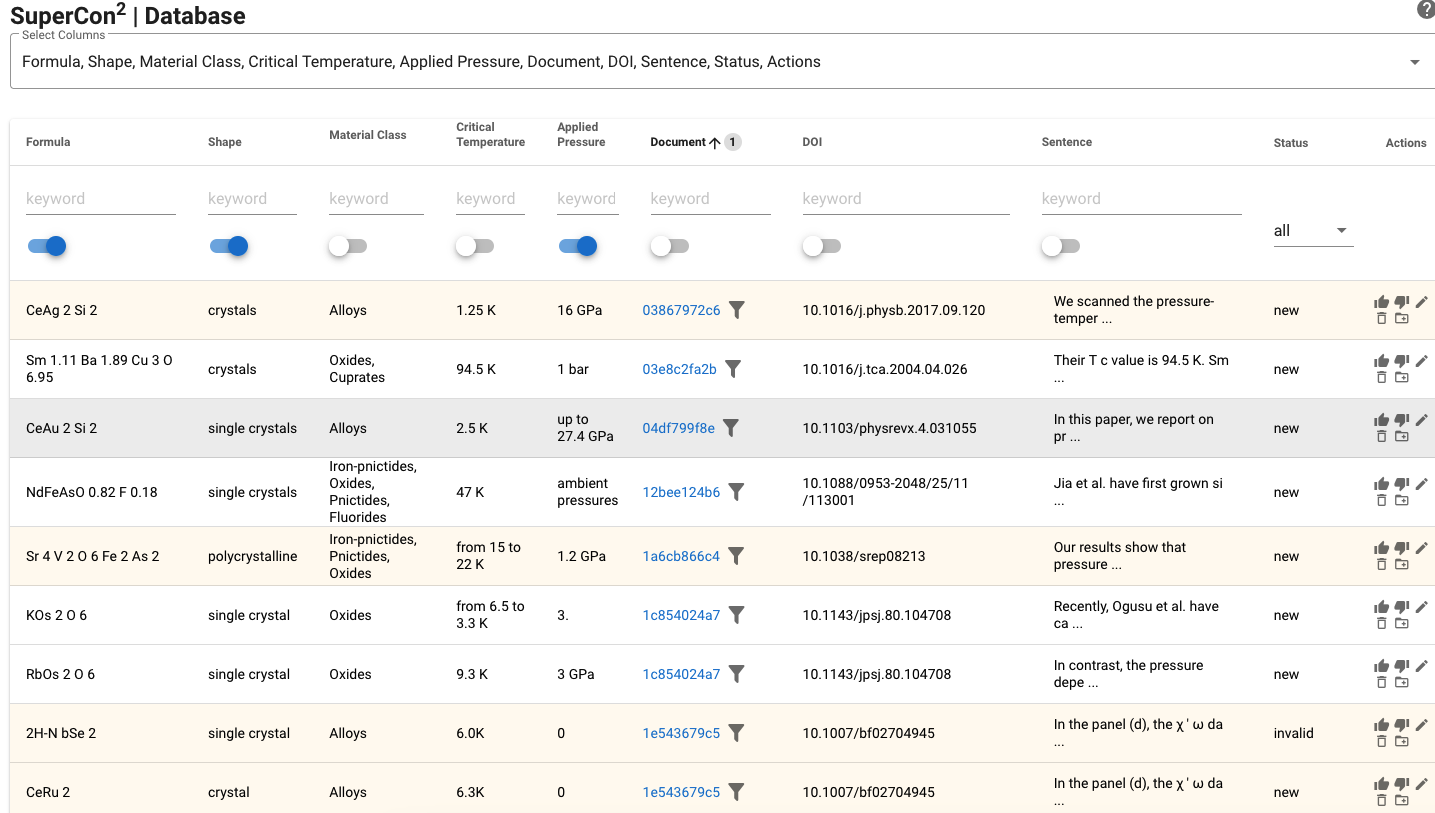
\includegraphics[width=1\textwidth]{figures/curation/supercon-curation-database.png} 
  \caption{Screenshot of SuperCon\textsuperscript{2} interface showing the database. Each row corresponds to one material-T\textsubscript{c} pair. On top, there are searches by attribute, sorting and other filtering operations. On the right (last column) there are curation controls (mark as valid, update, etc.).   Records are grouped by document with alternating light yellow and white. }
  \label{fig:curation-interface-database}
\end{figure}

During the curation process, it is often necessary to switch back and forth between the database record and the related context in the paper (the related paragraph or sentence). 
Our interface provides a viewer for individual documents, which visualises in the same window a table with the extracted records and the original PDF document decorated with annotations that identify the extracted materials and properties (Figure~\ref{fig:pdf-view}). 

\begin{figure}[ht]
  \centering
  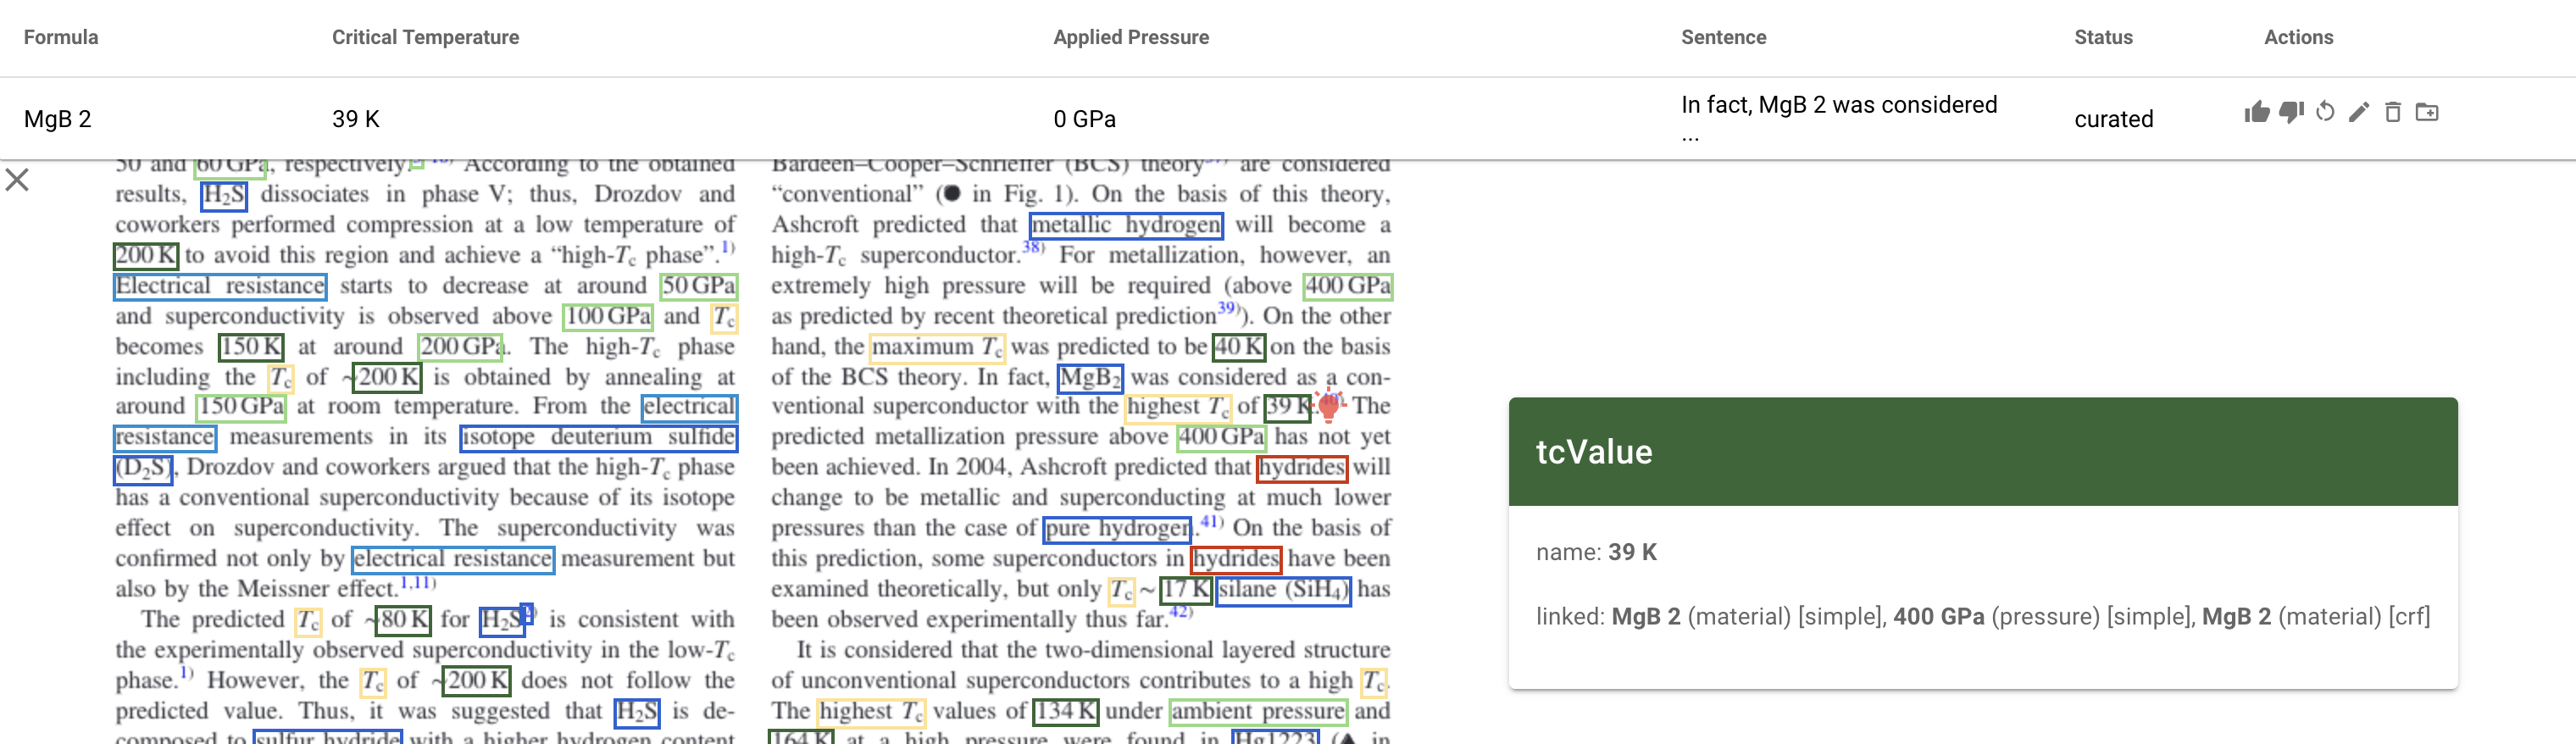
\includegraphics[width=1\textwidth]{figures/curation/pdf-view-context.png} 
  \caption{PDF document viewer showing an annotated document. The table on top is linked through the annotated entities. The user can navigate from the record to the exact point in the PDF, with a pointer (the red bulb light) identifying the context of the entities being examined. }
  \label{fig:pdf-view}
\end{figure}

% Through the interface, users can transition the record through the workflow as previously described . 
% Adding new records is limited to documents already in the database. When a record is added to a document, the record's bibliographic data are copied from other records in the same documents and the user has to only fill up the correct experimental information (material, Tc, etc.).


% The interface automatically collects training data; when a record is amended, the information pertaining it's raw source information (sentence text, annotations) is collected (Section~\ref{subsec:feedback-loop-training-data}). 

% \begin{figure}[ht]
%   \centering
%   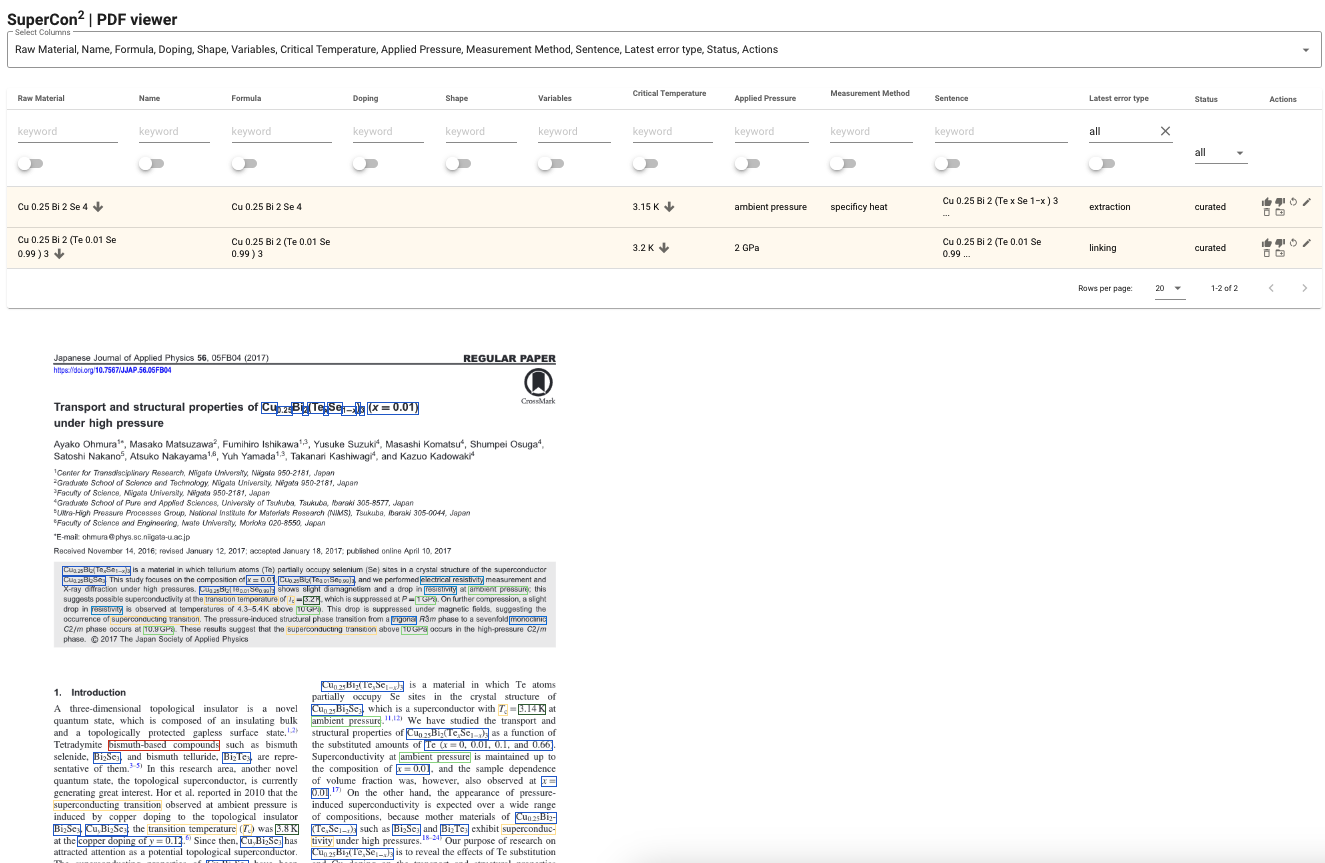
\includegraphics[width=1\textwidth]{figures/curation/supercon-curation-pdf-viewer} 
%   \caption{PDF viewer. The page includes a table showcasing records extracted from the  current document, along with the PDF content and accompanying annotations.}
%   \label{fig:curation-interface-pdf-viewer}
% \end{figure}


\subsection{Manual curation approach}
\label{sec:data-correction}
\label{subsec:manual_correction}

In this section, we discuss our strategy concerning manual curation, which is still indispensable for developing high-quality structures. 
% from automatically may contain incorrect information.
% We have set up an automatic process for anomaly detection (Section~\ref{subsec:anomaly-detection}) which can help to speed up the process but it only detects "potential" problems and requires anyway a manual validation.

We selected curators from domain experts in the field, to certify sufficient data quality. 
Nevertheless, as confirmed from our experiment in Section~\ref{sec:interface-evaluation}, the experience of each individual may have an impact on the final result.
We followed two principles to guarantee robustness in the curation process. 
First, we built solid curation documentation as a form of example-driven guidelines with an iterative approach we first introduced in \cite{foppiano2021supermat}. 
Then, we used a double-round validation approach, in which the data was initially corrected by one person, and validated in a second round, by a different individual. 

% The guidelines are included in the supporting material at the end of the manuscript.

% The loop includes four steps: 
% \begin{itemize}
%     \item collect rules, based on observation and reasoning,
%     \item curation following those rules,
%     \item retrospective including analysis and discussions based on curators' feedback, and
%     \item take decisions and update the guideline
% \end{itemize}

\subsection{Curation guidelines}
\label{subsec:curation-guidelines}

The guidelines consist mainly of two parts: the general principles and the correction rules with examples of solutions.
The guidelines are designed to provide general information applied to corrections and very basic explanations containing illustrations for a faster understanding (e.g. the meaning of the colours of the annotations). 
% This helps new curators catch up with the required level of curation precision quickly. 
Differently from our previous work~\cite{foppiano2021supermat}, these guidelines are divided into examples for different scenarios based on the error types mentioned in Section~\ref{subsec:error-types}.
Each example described the initial record, its context, the expected corrected record and a brief explanation, as illustrated in Figure~\ref{fig:example-curation-sheet}. 

\begin{figure}[ht]
  \centering
  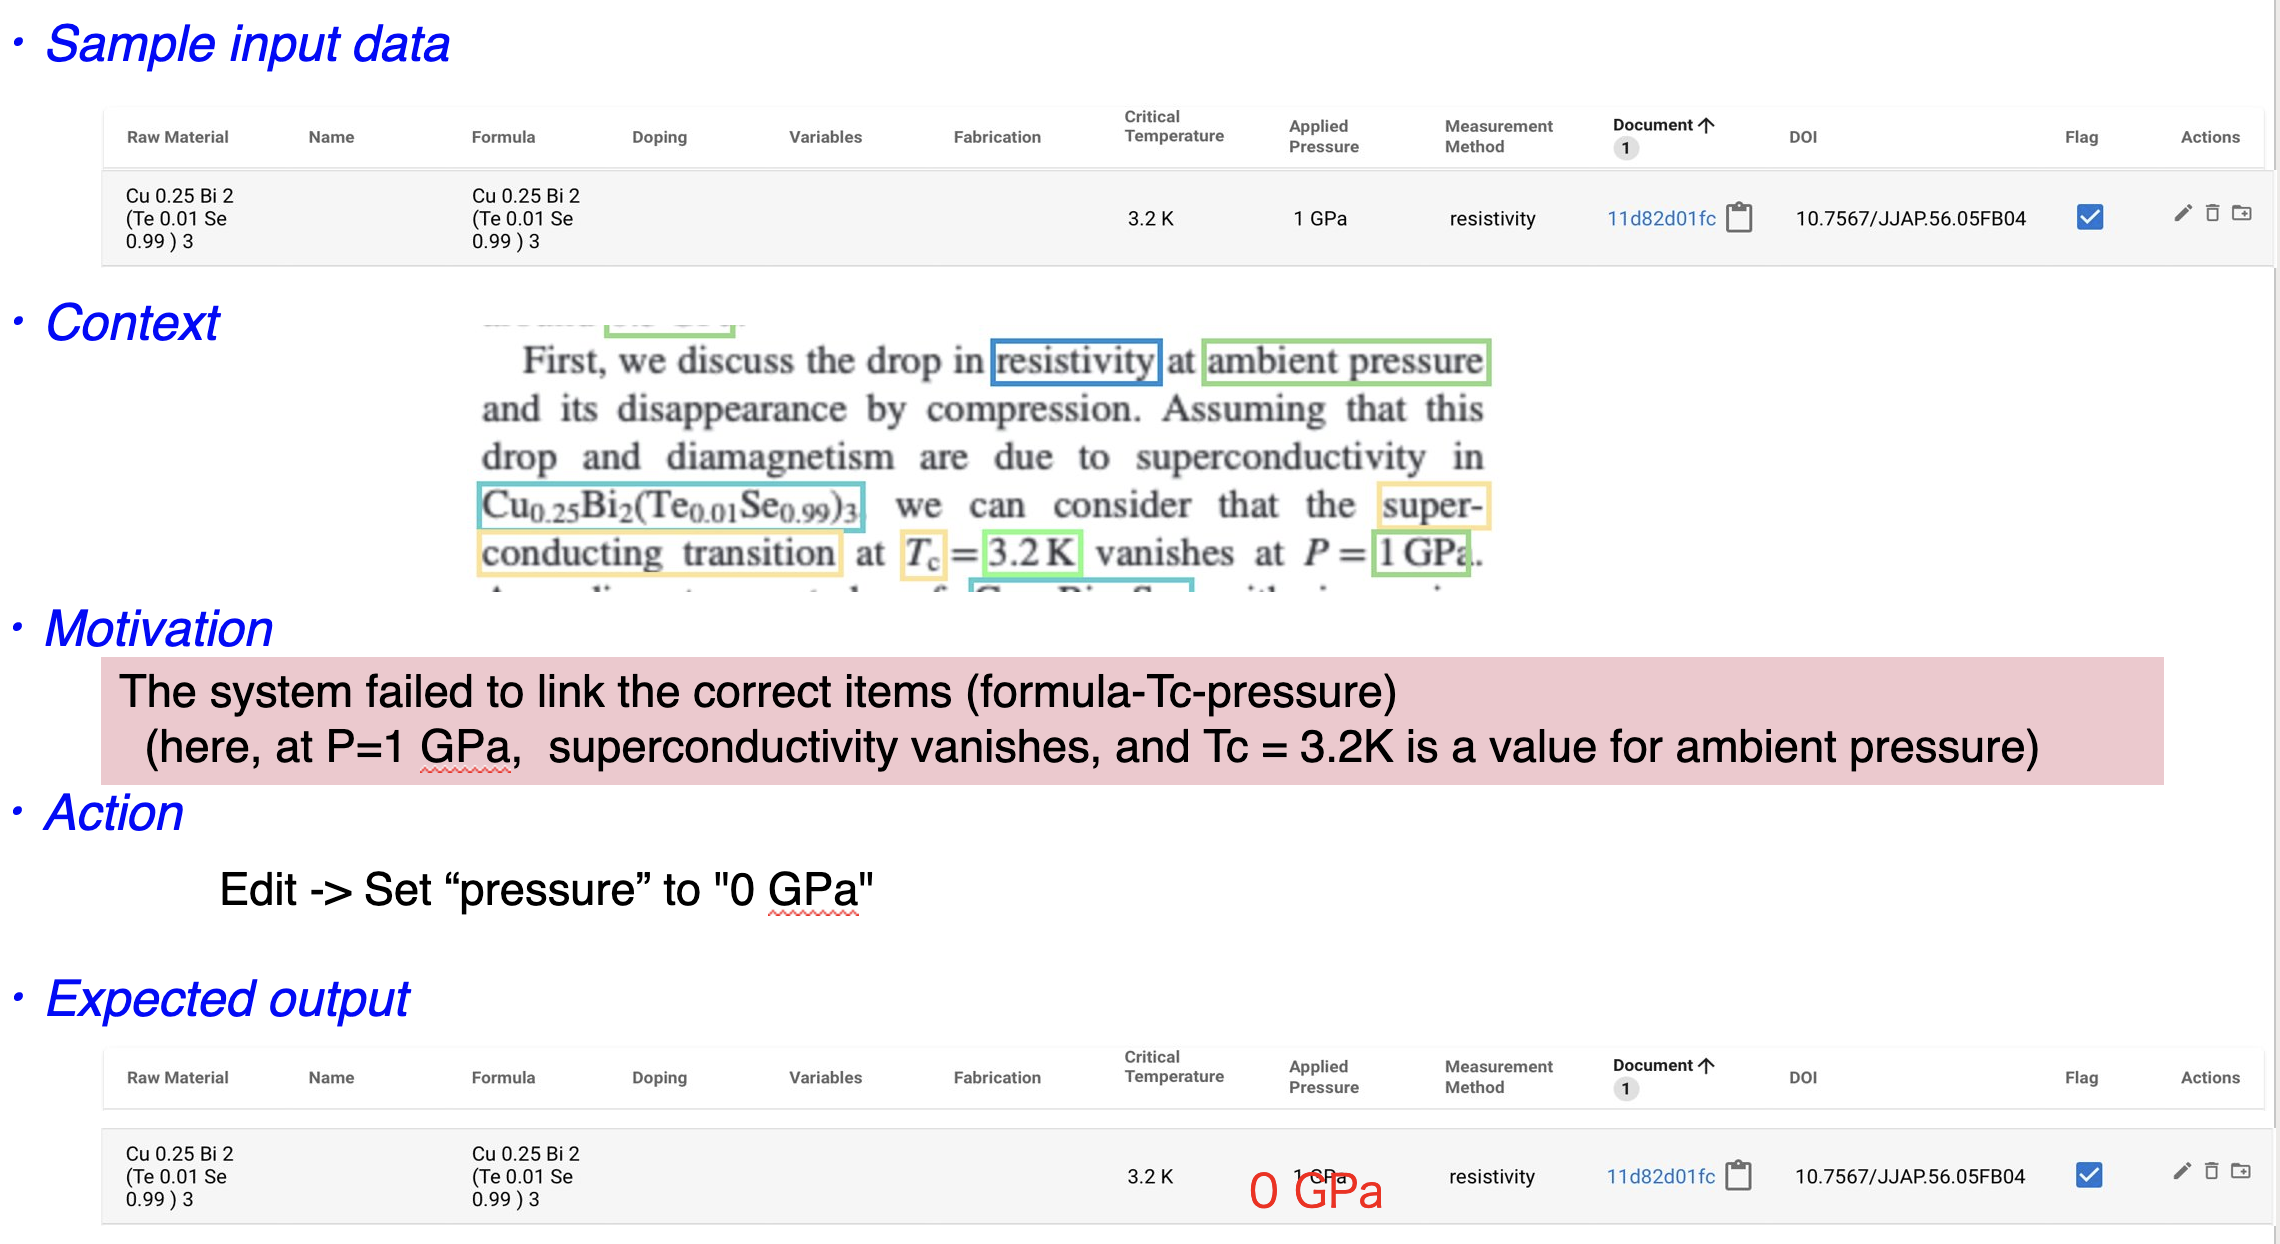
\includegraphics[width=1\textwidth]{figures/curation/example-sheet-curation.png} 
  \caption{Sample curation sheet from the curation guidelines. The sheet is composed of the following information: a) {Sample input data}: a screenshot of the record from the ``SuperCon\textsuperscript{2} Interface'', b) \textit{Context} represented by the related part of the annotated document referring to the record in exams. c) The \textit{Motivation}, describing the issue, d) the \textit{Action} to be taken, and the \textit{Expected output}.
 }
  \label{fig:example-curation-sheet}
\end{figure}



\subsection{Curation and processing logs}
\label{subsec:curation-and-processing-logs}

The Supercon\textsuperscript{2} interface gives access to information regarding the ingestion (processing log) and the curation process (curation log). 
The processing log is filled up when the new data is ingested, it was built to have minimal functions able to explain why certain documents haven't been processed (Figure~\ref{fig:processing-curation-log} top). 
For example, sometimes documents fail because they don't contain any text (image PDF documents) or they are too big (more than 100 pages). 
% Grobid was built focusing on speed and robustness, and contains several fail-safe mechanisms to avoid crashing the system when a document is either too big or does not contains valuable information, for example, does not have any text. 
% Old PDF documents (e.g. before 1990) are likely to have been scanned and contain only images. 
% Examples of too big documents are dissertation theses with more than 100 pages, that might be collected by mistake. 

\begin{figure}[ht]
  \centering
  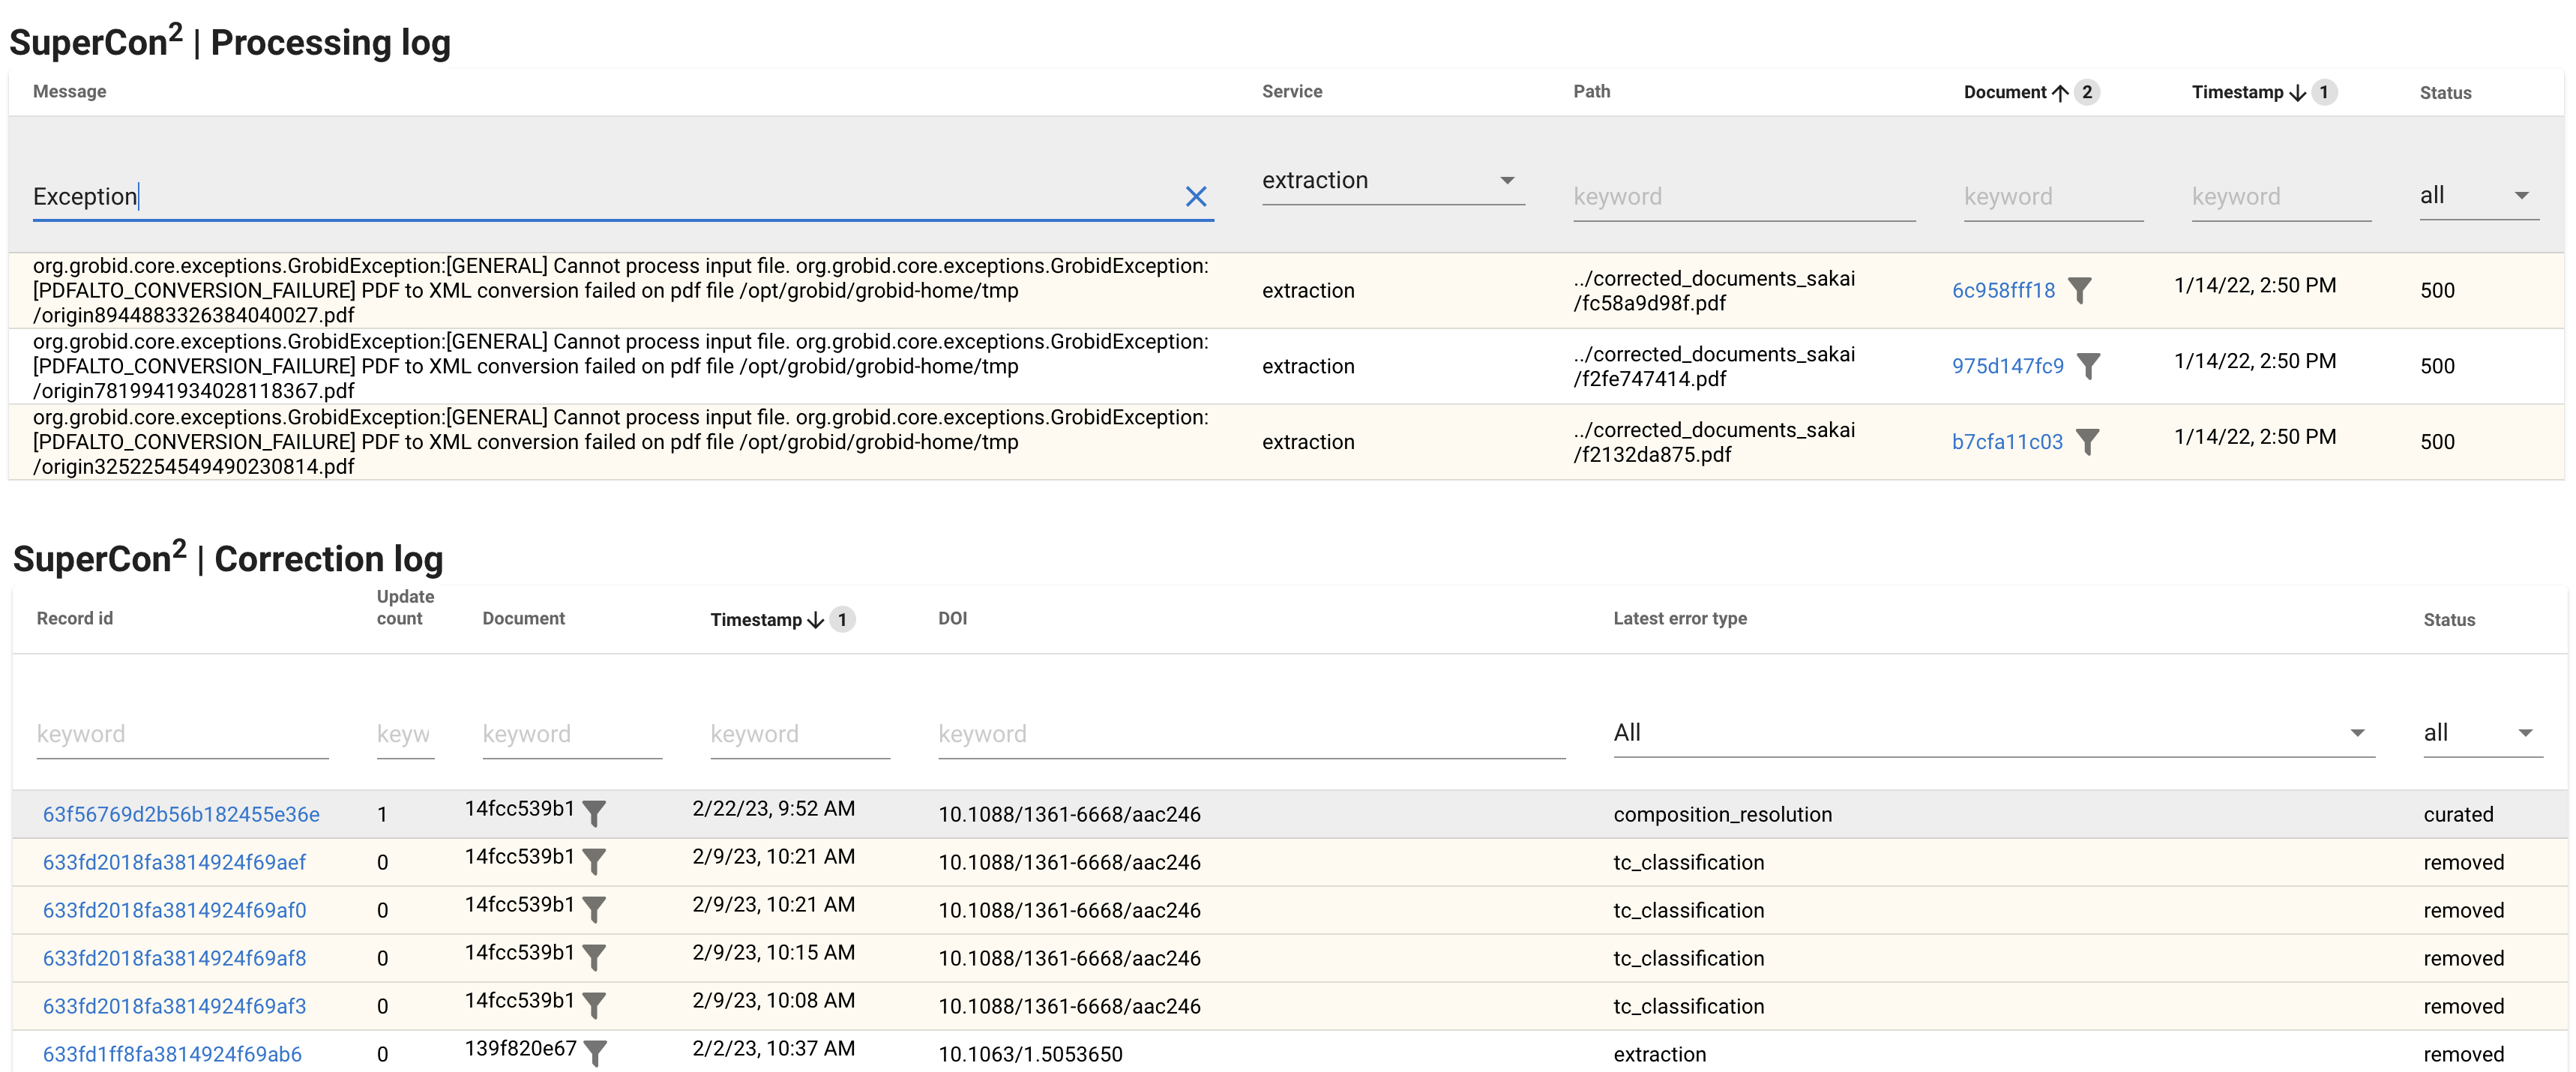
\includegraphics[width=1\textwidth]{figures/curation/processing-curation-log.png} 
  \caption{Top: \textit{Processing log}, showing the output of each ingestion operation and the outcome with the detailed error that may have occurred. Bottom: \textit{Correction log}, indicating each record, the number of updates, and the date/time of the last updates. By clicking on the ``Record id'', is possible to visualise the latest record values.}
  \label{fig:processing-curation-log}
\end{figure}

The curation log provides a view of what, when and how a record has been corrected (Figure~\ref{fig:processing-curation-log} bottom).

% \begin{figure}[ht]
%   \centering
%   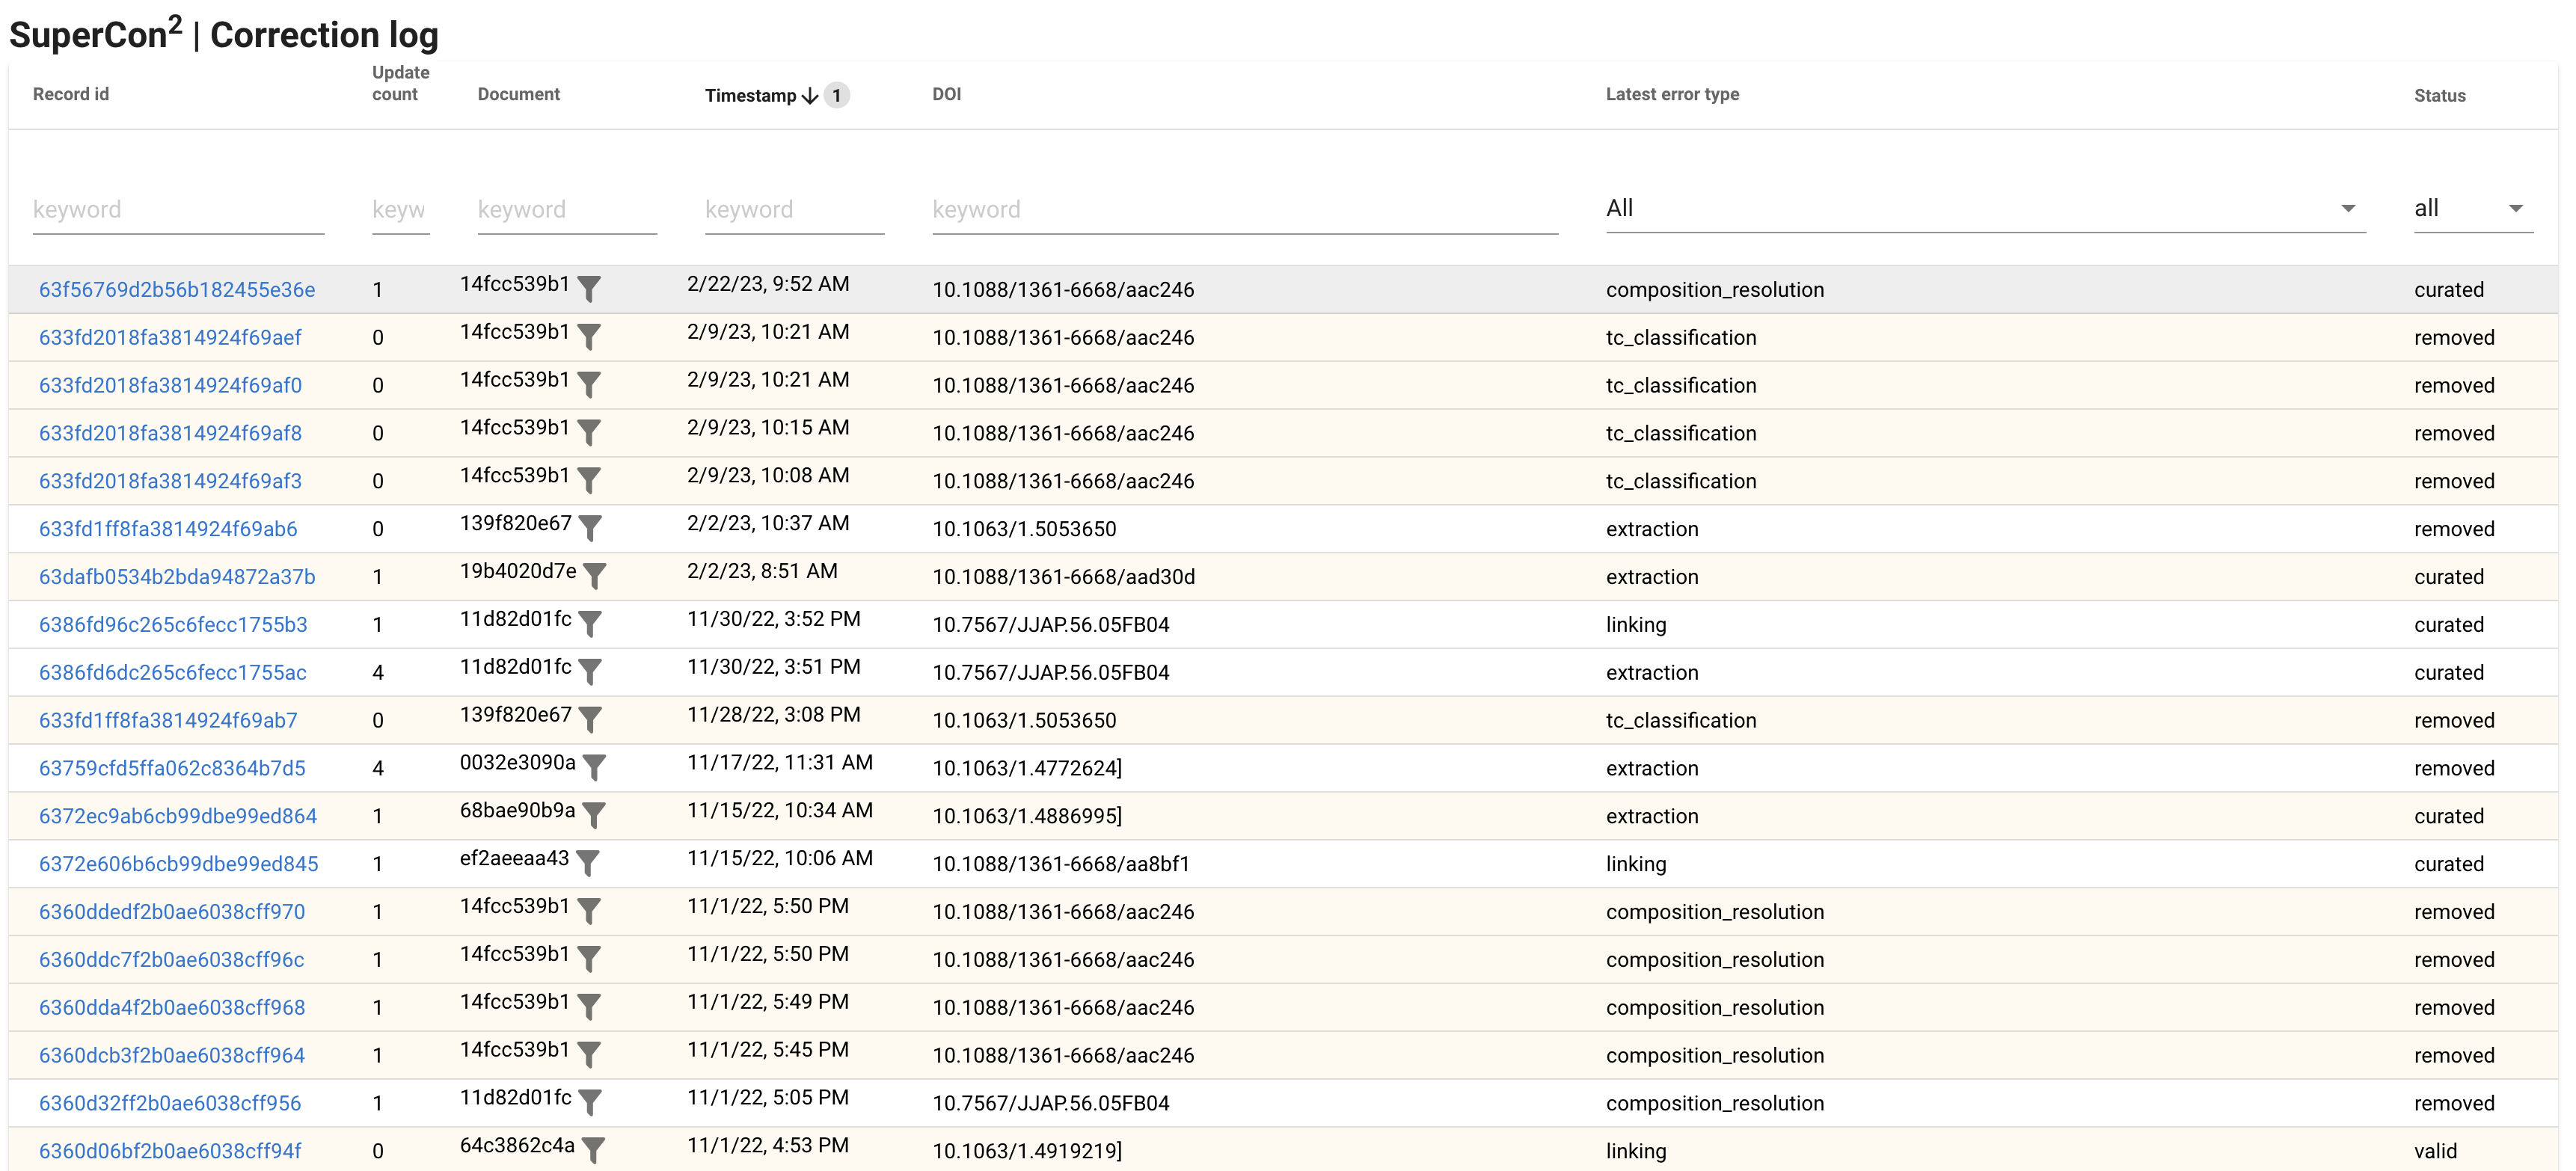
\includegraphics[width=1\textwidth]{figures/curation/curation-log} 
%   \caption{Curation log, indicating each record, the number of updates, and the date/time of the last updates. }
%   \label{fig:curation-log}
% \end{figure}

\section{Results and evaluation}
\label{sec:results-and-evaluation}

In this section, we illustrate the experiments we have run to evaluate our work. 
The evaluation is composed of three sets of results. 
The anomaly detection rejection rate (Section~\ref{subsec:anomaly-detection-evaluation}) indicates how many anomalies were rejected by curators after validation. 
Then, we demonstrate that the training data automatically selected contributed to improving the ML model with a small set of examples (Section~\ref{subsec:training-data-generation-evaluation}) 
Finally, we evaluated the quality of the data extraction using the interface (and the semi-automatic TDM process) against the classical method of reading the PDF articles and noting the experimental information in an Excel file. In Section~\ref{sec:interface-evaluation} we find out that using the interface improves the quality of the curated data by reducing missing experimental data. 


\subsection{Anomaly detection rejection rate}
\label{subsec:anomaly-detection-evaluation}

We evaluated the anomaly detection by observing the ``rejection rate'' which consists of the number of detected anomalies that were rejected by human validation. 
Running the anomaly detection on a database subset with 667 records, it found 17 anomalies in T\textsubscript{c}, 1 anomaly in applied pressure, and 16 anomalies in the chemical formulas. 
Curators examined each reported record and rejected 4 (23\%) anomalies in T\textsubscript{c}, 6 anomalies (37\%) in chemical formulas and 0 anomalies in applied pressure. 
This indicates an appropriate low rate of false positives although a study with a larger dataset might be necessary. 

\subsection{Training data generation}
\label{subsec:training-data-generation-evaluation}
We selected around 400 records in the Supercon\textsuperscript{2} Database that were marked as invalid by the anomaly detection process and we corrected them following the curation guidelines (Section~\ref{subsec:curation-guidelines}).
Then, we examined the corresponding training data corrected by the interface (Section~\ref{subsec:feedback-loop-training-data}) and obtained a set of 352 training data examples for our ML models. 
We call the obtained dataset \emph{curation} to be distinguished from the original SuperMat dataset which is referred to as \emph{base}.

We prepared our experiment using SciBERT~\cite{Beltagy2019SciBERT} that we fine-tuned for our downstream task as in~\cite{foppiano2023automatic}. 
We trained five models that we evaluated using a fixed holdout dataset from SuperMat averaging the results to smooth out the fluctuations. 
We use the DeLFT (Deep Learning For Text)~\cite{DeLFT} library for training, evaluating, and managing the prediction models.  
A model can be trained with two different strategies: 
\begin{enumerate}
    \item \emph{``from scratch''}: when the model is initialised randomly. We denote this strategy with an \emph{(s)}.
    \item \emph{``incremental''}: when the initial model weights are taken from an already existing model. We denote this strategy with an \emph{(i)}.
\end{enumerate}
The latter can be seen as a way to ``continue'' the training from a specific checkpoint.
We thus define three different training protocols: 
\begin{enumerate}
    \item \textbf{base(s)}: using the \emph{base} dataset and training from scratch (s).
    \item \textbf{(base+curation)(s)}: using both the \emph{base} and \emph{curation} datasets and training from scratch (s).
    \item \textbf{base(s)+(base+curation)(i)}: Using the \emph{base} dataset to train from scratch (s), and then continuing the training with the \emph{curation} dataset (i).
\end{enumerate}
We merge ``curation'' with the base dataset because the curation dataset is very small compared to ``base'', and we want to avoid catastrophic forgetting~\cite{overcoming-kirkpatrick-etal-2016} or overfitting.

\begin{table}[ht]
\centering\small
\caption{F1-score from the evaluation of the fine-tuned SciBERT models. The training is performed with three different approaches. 
The \emph{base} dataset is the original dataset described in~\cite{foppiano2021supermat}, and the \emph{curation} dataset is automatically collected based on the database corrections by the interface and manually corrected. \textit{s} indicate ``training from scratch'', while \textit{i} indicate ``incremental training''. 
The evaluation is performed using the same holdout dataset from SuperMat~\cite{foppiano2021supermat}. 
The results are averaged over 5 runs or train and evaluation. }
\begin{tabular}{lrrr}
\toprule
& \textbf{base(s)} & \textbf{(base+curation)(s)} & \textbf{base(s)+(base+curation)(i)} \\ 
\midrule
Nb total examples & 16902 & 17254 & 16902(s), 17254 (i)\\ 
\midrule
\texttt{<class>}        & 70.41         & \textbf{73.02}         & 71.86 \\ 
\texttt{<material>}     & 79.37         & 80.09         & \textbf{80.37} \\ 
\texttt{<me\_method>}   & 66.72         & 66.57         & \textbf{66.95} \\ 
\texttt{<pressure>}     & 46.43         & \textbf{48.42}         & 47.23 \\ 
\texttt{<tc>}           & 80.13         & \textbf{80.92}         & 80.34 \\ 
\texttt{<tcValue>}      & 78.29         & 78.41         & \textbf{79.73} \\ 
\midrule
\textbf{All (micro avg.)} & 76.67       & 77.44         & \textbf{77.48} \\ 
\midrule
\textbf{$\Delta$ avg. w/ baseline}& -   & +0.77     & \textbf{+0.81} \\ 
\bottomrule
\end{tabular}
\label{tab:evaluation-curation-training2}
\end{table}


The trained models are then tested using a fixed holdout dataset that we designed in our previous work~\cite{foppiano2023automatic} and the evaluation scores are shown in Table~\ref{tab:evaluation-curation-training2}.

This experiment demonstrates that with only 352 examples (2\% of the SuperMat dataset) comprising 1846 additional entities (11\% of the entities from the SuperMat dataset) (Table~\ref{tab:training-support}), we obtain an improvement of F1-score from 76.67\%\footnote{In our previous work~\cite{foppiano2023automatic} we reported 77.03\% F1-score. 
There is a slight decrease in absolute scores between DeLFT 0.2.8 and DeLFT 0.3.0. 
One cause may be the use of different hyperparameters in version 0.3.0 such as batch size and learning rate.
However, the most probable cause could be the impact of using the Huggingface tokenizers library which is suffering from quality issues \url{https://github.com/kermitt2/delft/issues/150}.} to values between 77.44\% (+0.77) and 77.48\% (+0.81) for (base+curation)(s) and base(s)+(base+curation)(i), respectively. 


\begin{table}[ht]
\centering
\small
\caption{Data support, the number of entities for each label in each of the datasets used for evaluating the ML models. The \emph{base} dataset is the original dataset described in~\cite{foppiano2021supermat}, and the \emph{curation} dataset is automatically collected based on the database corrections by the interface and manually corrected.}
\begin{tabular}{lccc}
\toprule
                        & \textbf{base}     & \textbf{base+curation}    & \textbf{$\Delta$}  \\ 
\midrule
\texttt{<class>}        & 1646              & 1732                      &  86                \\
\texttt{<material>}     & 6943              & 7580                      &  637               \\
\texttt{<me\_method>}   & 1883              & 1934                      &  51                \\
\texttt{<pressure>}     & 274               & 361                       &  87                \\
\texttt{<tc>}           & 3741              & 4269                      &  528               \\
\texttt{<tcValue>}      & 1099              & 1556                      &  457               \\
\midrule
\textbf{Total}          & 15586             & 17432                     & 1846               \\ 
\bottomrule
\end{tabular}
\label{tab:training-support}
\end{table}

% Here, the incremental approach obtained a score similar to the model trained from scratch with the extended ``base+curation'' dataset. 
% There are several hypotheses for this result, the first hypothesis is that the training dataset is not big enough for the task at hand, therefore the model requires more training time. 
% This issue could be verified by correcting all the available training data and repeating this experiment. 
% Another hypothesis that our data distribution is rather skewed (c.f. Table \ref{tab:training-support}) favours an incremental approach as the deltas in the support of the ``curation'' dataset with respect to the ``base'' dataset, somehow counters the class imbalance. 

This experiment gives interesting insight relative to the positive impact on the way we select the training data. 
However, there are some limitations: the \emph{curation} dataset is small compared to the \emph{base} dataset. This issue could be verified by correcting all the available training data, repeating this experiment, and studying the interpolation between the size of the two datasets and the obtained evaluation scores. 
A second limitation is that the hyperparameters we chose for our model, in particular, the learning rate and batch size could be still better tuned to obtain better results with the second and third training protocols.


\subsection{Data quality}
\label{sec:interface-evaluation}
We conducted an experiment to evaluate the effectiveness and accuracy of data curation using two methods: a) the user interface (\textit{interface}), and b) the ``traditional'' manual approach consisting of reading PDF documents and populating an Excel file (\textit{PDF documents}).

We selected a dataset of 15 papers, which we assigned to three curators — a senior researcher (SD), a PhD student (PS), and a master's student (MS). 
Each curator received 10 papers: half to be corrected with the \textit{interface} and half with the \textit{PDF Document} method. 
Overall, each pair of curators had 5 papers in common which they had to process using opposite methods.
For instance, if curator A receives paper 1 to be corrected with the \textit{interface}, curator B, who receives the same paper 1, will correct it with the \textit{PDF document} method.
After curation, a fourth individual manually reviewed the curated content. The raw data is available in the Appendix~\ref{app:interface-evaluation-raw}.

We evaluated the curation considering a double perspective: time and correctness. 
Time was calculated as the accumulated minutes required using each method. 
Correctness was assessed using standard measures such as precision, recall, and the F1-score.
Precision measures the accuracy of the extracted information, while recall assesses the ability to capture all expected information. F1-Score is a harmonic means of precision and recall. 

\begin{table}[ht]
\centering\small
\caption{Evaluation scores (P: precision, R: recall, F1: F1-score) between the curation using the SuperCon\textsuperscript{2} interface (\textit{Interface}) and the traditional method of reading the PDF document (\textit{PDF document}). }
\begin{tabular}{lrrrr}
\toprule
    \textbf{Method}    & \textbf{P (\%)}   & \textbf{R (\%)}   & \textbf{F1 (\%)}  & \textbf{\# docs}   \\
    \midrule
    PDF document    & 87.83             & 45.61             & 52.67             & 15        \\
    Interface       & \textbf{93.38}    & \textbf{92.51}    & \textbf{92.02}    & 15        \\
    \bottomrule
\end{tabular}
\label{tab:evaluation-interface-correction}
\end{table}


\subsubsection{Discussion}
Overall, both methods required the same accumulated time: 185 minutes using the \textit{interface} and 184 minutes using the \textit{PDF Document} method.
When the experiment was carried out, not all the curators were familiar with the \textit{interface} method. Although they had access to the user documentation, they had to get acquainted with the user interface, thus the accumulated 185 minutes included such activities. 

\begin{table}[h]
\centering
\caption{Evaluation scores (P: precision, R: recall, F1: F1-score) aggregated by experience (MS: master student, PD: PhD student, SR: senior researcher). Each person corrected 10 documents.}
\begin{tabular}{lrrrrr}
\toprule
\textbf{Experience} & \textbf{P (\%)}   & \textbf{R (\%)}   & \textbf{F1 (\%)}  & \textbf{\#  docs} & \textbf{\# pages}\\
\midrule
MS      & 90.03             & 60.26             & 64.50           & 10  & 96    \\
PD      & 83.33             & 65.69             & 69.45           & 10  & 100   \\
SR      & \textbf{98.45}    & \textbf{81.22}    & \textbf{83.08}  & 10  & 96  \\
\bottomrule
\end{tabular}
\label{tab:accuracy-by-experience}
\end{table}

We examined the quality of the extracted data and we observed an improvement of +5.55\% in precision and a substantial +46.69\% in recall when using the \textit{interface} as compared with the \textit{PDF Document} method (Table~\ref{tab:evaluation-interface-correction}). 
The F1-score improved by 39.35\%.

The disparity in experience significantly influenced the accuracy of curation, particularly in terms of high-level skills. Senior researchers consistently achieved an average F1-Score approximately 13\% higher than other curators (see Table~\ref{tab:accuracy-by-experience}). Furthermore, we observed a modest improvement between master's students and PhD students. These findings indicate also that for large-scale projects, employing master students instead of PhD students may be a more cost-effective choice. Thus, using only a few senior researchers for the second round of validation (Section~\ref{subsec:manual_correction}).

\begin{table}[h]
\centering\small
\caption{Evaluation scores (P: precision, R: recall, F1: F1-score) listed by experience (MS: master student, PD: PhD student, SR: senior researcher), and method (PDF document, Interface). }
\begin{tabular}{lcrrrrr}
\toprule
\textbf{Experience} & \textbf{Method} & \textbf{P (\%)} & \textbf{R (\%)} & 
\textbf{F1 (\%)}  & \textbf{\# docs} & \textbf{\# pages}\\
\midrule
\multirow{2}{*}{MS} & PDF Document & 94.58 & 36.55 & 48.67 & 6 & 46 \\
 & Interface & 83.19 & 95.83 & 88.25 & 4 & 50 \\
\midrule
\multirow{2}{*}{PD} & PDF Document & 70.00 & 48.51 & 50.78 & 5 & 49 \\
 & Interface & 96.67 & 82.86 & 88.11 & 5 & 51\\
\midrule
\multirow{2}{*}{SR} & PDF Document & \textbf{100.00} & 55.56 & 61.03 & 4 & 51\\
 & Interface & 97.42 & \textbf{98.33} & \textbf{97.78} & 6 & 45\\
\bottomrule
\end{tabular}
\label{tab:accuracy-by-experience-method}
\end{table}

Finally, the collected data suggest that all three curators had overall more corrected results by using the interface as illustrated in Table~\ref{tab:accuracy-by-experience-method}. 

The results of this experiment confirmed that our curation interface and workflow significantly improved the quality of the extracted data, with an astonishing improvement in recall, thus preventing curators from overlooking important information.

\section{Code availability}
This work is available at \url{https://github.com/lfoppiano/supercon2}. The repository contains the code of the SuperCon\textsuperscript{2} interface, the curation workflow, and the ingestion processes for harvesting the SuperCon\textsuperscript{2} Database of materials and properties. The guidelines are accessible at \url{https://supercon2.readthedocs.io}.




\chapter{Conclusion}
We propose an end-to-end pipeline for extracting material information from the scientific literature to improve the efficiency and quality of materials databases.

In Chapter~\ref{cha:automatic} we described the automatic system that reads PDF documents, extracts information and stores them in a tabular format where each entry represents a material and its related properties (\tc, applied pressure, measurement methods, etc.) using a combination with Grobid-quantities: a general system for identification and standardisation of physical quantities and measurements, described in Chapter~\ref{cha:measurements}.
ML models have been trained and evaluated using SuperMat (Chapter~\ref{cha:supermat}), a dataset we developed with domain experts that provides annotations and relations between entities in 142 scientific documents from superconductor research.

Material expressions are carefully managed with a specific material parser that combines different methods to decompose mixed information (doping, shape, formula, name, etc.). 
Using this framework We automatically collected from 37000 articles a "SuperCon\textsuperscript{2} Database" containing 40324 records of materials and properties.

In Chapter~\ref{cha:curation} we described a staging area using the obtained "SuperCon\textsuperscript{2} Database" with machine-collected entities. Using a user interface "SuperCon\textsuperscript{2} Interface", we allow domain experts to examine and correct the data by accessing the exact location in the original PDF document decorated with the extracted information. 
Our interface significantly improves the curation quality by increasing both precision and recall by approximately 6\% and +47\%, respectively.


% \chapter*{Acknowledgements}
% \addcontentsline{toc}{chapter}{Acknowledgements}
\newpage

\addcontentsline{toc}{chapter}{Bibliography}
\bibliographystyle{unsrt}
\bibliography{references.bib}


\end{document}